\documentclass[12pt,spanish,hidelinks,BCOR=5cm]{scrbook} %\usepackage{charter} % Use the Charter font
\usepackage{hyperref} 
\hypersetup{%
  colorlinks=false,% hyperlinks will be coloured
  linkcolor=black,% hyperlink text will be green
}
\usepackage[
	a4paper, % Paper size
	top=1in, % Top margin
	bottom=1in, % Bottom margin
	left=1in, % Left margin
	right=1in, % Right margin
	%showframe % Uncomment to show frames around the margins for debugging purposes
]{geometry}
\setlength{\parindent}{0pt} % Paragraph indentation
\setlength{\parskip}{1em} % Vertical space between paragraphs
\usepackage{graphicx} % Required for including images
\usepackage{fancyhdr} % Required for customizing headers and footers

\fancypagestyle{firstpage}{%
	\fancyhf{} % Clear default headers/footers
	\renewcommand{\headrulewidth}{0pt} % No header rule
	\renewcommand{\footrulewidth}{1pt} % Footer rule thickness
}

\fancypagestyle{subsequentpages}{%
	\fancyhf{} % Clear default headers/footers
	\renewcommand{\headrulewidth}{1pt} % Header rule thickness
	\renewcommand{\footrulewidth}{1pt} % Footer rule thickness
}

\AtBeginDocument{\thispagestyle{firstpage}} % Use the first page headers/footers style on the first page
\pagestyle{subsequentpages} % Use the subsequent pages headers/footers style on subsequent pages
 openany,
\KOMAoptions{DIV=calc}
% \setlist[itemize]{noitemsep, topsep=0pt}
\usepackage[a5paper]{geometry}%landscape
\usepackage[utf8]{inputenc} % \usepackage{kpfonts,baskervald}
\usepackage[spanish]{babel}
\selectlanguage{spanish}
\usepackage{mdframed} %for text in box through pages
\usepackage{lipsum}   %for text in box through pages
\usepackage{amsmath}   %for text in box
\usepackage{tcolorbox} %for text in box
\tcbuselibrary{breakable} % verbatim previous
\usepackage{ccicons}
\usepackage{ebgaramond}
% \usepackage{booktabs}
\usepackage[T1]{fontenc}
\usepackage{sectsty}
\chapterfont{\normalfont\itshape}
\usepackage{microtype} 
\usepackage{incgraph,tikz} 
\usepackage{wasysym} \usepackage{marvosym}
\usepackage{textcomp} \usepackage{amssymb}
\usepackage{makeidx} \usepackage{mdframed}
\usepackage{epigraph} \renewcommand{\textflush}{flushepinormal}
% \usepackage[hidelinks]{hyperref}
\usepackage{hyphenat} %no word break in epigraph
\setlength\epigraphwidth{8.5cm} 
\setlength\epigraphrule{0pt}

% https://tex.stackexchange.com/questions/311721/how-can-i-place-a-1-cm-margin-to-a-set-pdf-book-a6-to-print
\addtolength\oddsidemargin{1cm} \addtolength\evensidemargin{-1cm} 

\widowpenalty10000 
\clubpenalty10000

\newcommand\textlcsc[1]{\textsc{\MakeLowercase{#1}}}
\date{}
%\input{main-matter} 
\makeindex
\begin{document}
\newpage \thispagestyle{empty} \mbox{} \cleardoublepage

\begin{titlepage}\thispagestyle{empty} \vspace*{7em}{\centering\Huge \textsc{Tratado Sobre \\ el Amor} \par}\clearpage
\newpage \thispagestyle{empty} \mbox{} \cleardoublepage
\thispagestyle{empty} \vspace*{7em}{\centering\Huge \textsc{Tratado Sobre \\ el Amor} \par
%\begin{normalsize}como lo entiende una persona terriblemente aburrida \end{normalsize} \par
}
\centering{\Large \textsc{como lo entiende una persona \\ terriblemente aburrida} \par}
    \vspace*{1cm}
    {\centering {\LARGE -- Anatoliy Protopopov} \par}\cleardoublepage
\newpage \thispagestyle{empty} \mbox{} \clearpage
\vfill

\begin{mdframed} \begin{scriptsize} \noindent 
Autor: Anatoliy Protopopov \\ 
Título: Tratado Sobre el Amor. Como lo entiende una persona terriblemente aburrida\\
1\textsuperscript{era} edición. pasada por alto. \\ 
1. Etología 2. Animales 3. Ciencia 4. Instintios %5. Conducta humana 
\end{scriptsize} \end{mdframed}

% \vfill
% creative commons!
% \ccbyncnd


\thispagestyle{empty} \vspace*{\fill} \parbox{.8\textwidth}
% \noindent

{\raggedright %\ccbyncnd \\ 
\scriptsize
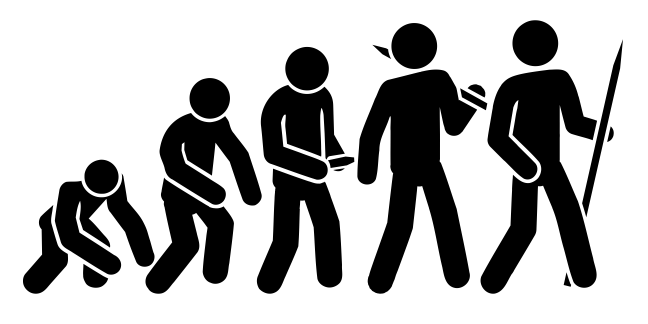
\includegraphics[width=0.1\textwidth]{logo.png} \\
ediciones \textit{intempestivas}  2017 \\
impreso en la oscuridad \\
diseño | \LaTeX \\

foto de Portada | Dean Nahum [Unsplash]\\
logo de edición | Jakob Vogel [Noun Project]\\
traducción del ruso | Irina Italianskaya \\%
%  \href{mailto:isabel@nubimar.com}{Irina Italianskaya.
 {\normalsize \ccbyncnd} \\ 
 }
}
\end{titlepage} 
\clearpage \thispagestyle{empty}\cleardoublepage

%%%%%%%%%%%%%%%%%% QUOTE %%%%%%%%%%%%%%%%%%%
\thispagestyle{empty}
\vspace*{\fill}
\epigraph{\hyphenpenalty10000 \exhyphenpenalty10000
Manual para los jóvenes que están desconcertados y cansados de las extrañezas del amor. Se contemplan las bases instintivas del comportamiento matrimonial del ser humano como especie biológica. Al principio brevemente se contemplan las condiciones biológicas, después se aclara la elección de la pareja matrimonial de la persona, se dan consejos prácticos. La redacción termina un resumen etológico de los motivos instintivos del comportamiento humano.} 

\vspace*{\fill} \cleardoublepage

\tableofcontents\thispagestyle{empty}
\clearpage \cleardoublepage 
\thispagestyle{empty}

\pagestyle{plain}

%\part{1} hey 

\vspace*{\fill}
\begin{raggedleft}
\textit{Todo lo real es razonable}.\\
\textit{Todo lo razonable es real}.\\
G. Hegel\\ \bigskip
\textit{La sabiduría real es el saber de las causas}.\\
(G. Galileo)\\
\end{raggedleft}
\vspace*{\fill}
\cleardoublepage


\subsubsection*{Breves palabras sobre la etología del ser humano}
\label{breves-palabras-sobre-la-etologia-del-ser-humano}
% \addcontentsline{toc}{subsubsection}{line added to TOC: subsubsection one}
\addcontentsline{toc}{subsubsection}{\protect\numberline{\thesubsubsection} line added to TOC: subsubsection one}
\addcontentsline{toc}{section}{Breves palabras sobre la etología del ser humano}

\noindent
Introduccion para la edición Bulgara del año 2002

~ ~ ~ A la psicología tradicional, así como otras ciencias que estudian
al ser humano, siempre le interesó la relación de la parte biológica y
no biológica en el comportamiento humano. En distintas épocas se
estudiaba como predominante ora la influencia biológica, ora no
biológica. En el siglo 19 y a principios del siglo 20 la opinión más
aceptada era la predominancia del componente biológico. Zigmund Freud
era el más famoso de los que expresaban tal opinión (aunque el no era el
único). Pero hablando siempre prácticamente de instintos (``libido'' y
``mortido'') y su influencia sobre el ser humano, el nunca hizo ningún
esfuerzo para estudiar su naturaleza física o génesis. No es de
sorprender que sus ideas no se percibían como muy convincentes, y
siempre se criticaban. Además, fundada en la paradigma muy similar,
eugenesia se desacreditó por la culpa de los regímenes despóticos que la
utilizaron como apoyo ideológico de la política de opresión. Por eso
desde los años 20 del siglo XX el péndulo se movió para otro lado,
pasando de largo, como suele suceder en estos casos, el justo medio.
Hasta hace poco reinó la teoría de la predominancia del componente
social en el comportamiento humano, algunas veces llamado concepto de la
``Tabula Rasa'', es decir; ``Hoja en Blanco''. Esta teoría supone que el
ser humano al nacer es como una hoja en blanco donde la sociedad y el
ambiente escriben unos u otros modos de comportamiento, y dependiendo de
qué va a escribirse así va a ser la persona. Pero con el transcurso del
tiempo se hizo más obvia la imposibilidad de explicar claramente y fácil
todos los matices de las reacciones del comportamiento humano. Al mismo
tiempo muchas inexplicables reacciones humanas se explican con mucha
naturalidad utilizando la hipótesis de la existencia en el ser humano de
una base muy amplia de esquemas innatos del comportamiento. Por eso ya a
finales del siglo XX los extremos empezaron a eliminarse, y el punto de
vista que el ser humano es un ser en gran parte biológico que nace con
una carga no despreciable de los esquemas predeterminados de conducta
empezó a obtener mayor apoyo. Quizá la aportación más grande en ello
realizó casi hace medio siglo la ciencia de etología y las asignaturas
que surgieron de ella. La etología estudia las bases instintivas de la
conducta de los seres vivos mediante el método de comparación del
comportamiento de distintas especies entre sí. El ser humano para un
etólogo es solamente un mamífero erguido, es decir, es uno entre los
mamiferos.\\
\hspace*{0.333em} ~ ~ Comparando entre sí la conducta de los
representantes de distintos tipos zoológicos desde los primitivos hasta
los superiores, los científicos descubren paralelismos sorprendentes que
atestiguan los principios de conducta comunes que conciernen a todos los
representantes del reino animal, entre ellos al ser humano. Los métodos
parecidos de estudiar el mundo son muy fructíferos y se utilizan
ampliamente en otras ciencias. Por ejemplo los astrónomos conocen mejor
la estructura interior del Sol que los geológos la estructura interior
de la Tierra. Y es que hay muchos astros y comparándolos entre sí se
pueden entender muchas cosas. La Tierra es única y no hay con qué
compararla. Eso pasa en los estudios del ser humano. Limitándose al
estudio de este mismo nos arriesgamos a limitarnos en su comprensión.\\
\hspace*{0.333em} ~ ~ Pero no es fácil estudiar la etologia. Además de
las dificultades objetivas que surgen de la enorme influencia de la
razon que enmascara y modifica muchas manifestaciones instintivas, los
científicos chocan con el rechazo del método etológico para el ser
humano. A muchos les parece inadmisible e inclusive ofensivo el hecho de
comparar la conducta humana con la animal. ¡Esto tiene su explicación
etológica! Se trata de la acción del instinto del aislamiento etológico
de las especies, el estudio detallado del cual sobrepasa los límites de
nuestro libro (los que quieran pueden leer el libro de V.Dolnik ``el
nino desobediente de la biósfera''). El principio de este instinto se
puede expresar con el lema: ``Ama al prójimo - odia al ajeno'', y
``ajenos'' en nuestro caso son los monos, la hostilidad a los cuales se
extiende a la tesis del parecido de nuestro comportamiento con su
comportamiento. Aunque la teoría de Darwin pese a todos los intentos
(debido a esta hostilidad) hasta hoy día de refutarla está admitida
irrevocablemente por la comunidad científica, y la mayoría de la gente
está de acuerdo de su procedencia de los monos, la idea de que uno u
otro sentimiento es la voz del instinto provoca en mucha gente protestas
airadas que no encuentran ninguna explicación racional. Pero la causa de
este rechazo está en el rechazo subconsciente de nuestro parentesco con
los monos. Recuerden eso, mis estimados lectores.\\
\hspace*{0.333em} ~ ~ ¿Qué más puede contar un etólogo sobre el ser
humano? Mucho. Sobre la agresividad, sobre la naturaleza del poder,
sobre la moralidad innata y las fuerzas motoras del nacionalismo e
inclusive sobre las extrañezas del amor. Y precisamente de las
extrañezas del amor vamos a hablar en este libro.

\protect\hypertarget{M1}{}{}

\subsubsection*{De qué se trata}
\label{de-quuxe9-se-trata}
\addcontentsline{toc}{section}{De qué se trata}

\noindent
\textit{Pregunta a la radio de Armenia:}\\
% \noindent
\textit{``¿Qué contraceptivo hay que utilizar?''}\\
\textit{Respuesta: ``Hay que tomar el agua mineral''.}\\
\textit{Pregunta: ``¿Cuándo, ANTES DE o DESPUÉS DE?''}\\
\textit{Respuesta: ``EN VEZ DE''.}\\
(un chiste viejo)\\
% 
% 

~ ~ ~ Los intentos de la sociedad de ilustrar a los jóvenes en materias
del sexo, en mi opinión, son extremadamente limitados. Ampliamente se
aclaran los problemas de la técnica del sexo, contracepción y
enfermedades. Desde luego, hablar sobre la técnica del sexo es muy
agradable, pero la mayoría de las tragedias en el terreno sexual ocurre
no porque SE HACE COMO NO SE DEBE, sino se hace CON QUIEN NO se debe. No
obstante, sobre la elección de la pareja se habla de paso, sin sistema,
con contradicciones, y, gracias a unos argumentos subjetivos y con mera
especulación, poco convincente. Realmente todo se traduce en un consejo
de vivir juntos mucho tiempo, y ``beber agua mineral''. Pero la larga
vida común no es una garantía que después todo vaya bien, y, mientras
tanto se pueden perder posibilidades, más de una, realmente válidas.\\
\hspace*{0.333em} ~ ~ Durante toda la historia escrita de la humanidad,
se consideraba oportuno guíarse durante la elección de pareja por el
sentimiento de amor, y los últimos decenios más todavía, el amor, como
conjuro, empezó a contraponerse a las pasiones momentáneas,
considerándose una garantía de infalibilidad de la elección. Pero hasta
el momento no está demostrado que esta confianza esté justificada, ya
que la diferencia entre el ``gran'' amor y una breve simpatía es
meramente cuantitativa, y no calificativa. En vez de esto se explican y
se describen de una manera muy pintoresca las sensaciones que aparecen
durante el estado de enamoramiento, pero la lógica básica queda al
margen, o simplemente se niega su existencia, y se contempla como algo
sobrenatural. Pero no se debe buscarse misterio donde no lo hay, todas
las cosas irracionales del amor en realidad son muy racionales, lógicas,
y razonables a su manera. Para ver esta racionalidad es necesario
solamente pasar a otro sistema de coordenadas, desde el civilizado al
prehistórico de una manada. Más abajo trataré de demostrar cómo hacerlo,
y demostrar que este paso es correcto. Concretamente, vamos a hablar de
la base instintiva del comportamiento matrimonial del ser humano como
especie biológica. El proceso del coito no vamos a examinar. Tampoco nos
va a interesar el SENTIMIENTO en sí, es decir, las sensaciones que
experimenta una persona enamorada, y mecanismos fisiológicos de su
aparición.\\
\hspace*{0.333em} ~ ~ Estoy convencido de que el saber de toda esta
lógica de ninguna manera va a empobrecer la percepción del amor como los
sentimientos más maravillosos, así como el saber la estructura de una
flor no impide al botánico admirar su belleza, y el saber de las leyes
de harmonía y la estructura de un instrumento no impide (e, incluso, le
ayuda) al músico a disfrutar cuando toca una obra maestra.\\
\hspace*{0.333em} ~ ~Las bases instintivas del comportamiento las estudia una
ciencia, la etología, pero prácticamente no existen ediciones populares
sobre el tema del comportamiento matrimonial del ser humano, y espero
que este artículo de algún modo va a llenar este vacío.

\protect\hypertarget{M1A}{}{}

\subsubsection{¿Y para qué, hablando con propiedad, multiplicarse?}
\label{y-para-quuxe9-hablando-con-propiedad-multiplicarse}
\addcontentsline{toc}{section}{¿Y para qué, hablando con propiedad, multiplicarse?}

\noindent 
\textit{Es comprensible la tristeza del que viene a este mundo.}\\
\textit{Debe volver a la inexistencia otra vez.}\\
(Omar Khaiam)\\

~ ~ ~ Durante la vida de cualquier ser viviente su material genético
paulatinamente está alterándose, se acumulan los fallos, y como
resultado de ello el organismo paulatinamente baja sus posibilidades de
supervivencia y al fin se muere. No vamos a examinar otras teorías del
envejecimiento, ya que eso sobrepasa los márgenes de nuestro tema. El
fenómeno de multiplicación de los organismos vivientes conocidos por
nosotros consiste en que los descendientes reciben los genes
prácticamente libres de estos fallos acumulados. En caso contrario los
hijos heredarían de sus padres no solamente peculiaridades de la
constitución corporal, pero también su edad, y el cambio generacional se
extinguiría rápidamente, y, mejor dicho, ni aparecería.

\begin{itemize}
% 
\item
  La multiplicación es el método de limpiar el material genético de los
  fallos, es decir, es un método de ``vivir eternamente''.
\end{itemize}

\protect\hypertarget{M2}{}{}

\subsubsection{Gemificación y proceso sexual}\label{gemificaciuxf3n-y-proceso-sexual}
\addcontentsline{toc}{section}{Gemificación y proceso sexual}

\noindent
\textit{La multiplicación es mejor hacerla por división.}\\
(de la charla de dos amebas)\\

~ ~ ~ La multiplicación vegetativa se limita a la simple división de la
célula, pero la división de la célula es un proceso muy complicado pese
a su simplicidad aparente. El texto genético no solamente se duplica,
después de la división los cromosomas ingeniosamente se intercambian de
distintas partes de las mismas; y, como resultado, los genes defectuosos
se suprimen y no se transmiten a los descendientes. Solamente después de
esto la célula se divide en dos. Pero existe una posibilidad bastante
alta de que todos los ejemplares del gen en los espirales del cromosoma
resulten dañados, y no habrá posibilidad de disponer de un gen sin
daños.\\
\hspace*{0.333em} ~ ~ Para excluir o bajar substancialmente la
incidencia de esta posibilidad, la naturaleza legó al proceso sexual. Su
principal diferencia del proceso vegetativo consiste en que se
intercambian con sus partes dos juegos genéticos no idénticos recibidos
de dos individuos diferentes, en los cuales prácticamente no hay
coincidencia de fallos en los genes. Además, aparece a posibilidad de
combinar en los descendientes características y particularidades
recibidas de los padres diferentes, que simplifica la adaptación al
medio ambiente.\\
\hspace*{0.333em} ~ ~ Es necesario pagar por las ventajas del proceso
sexual. El vegetativo es más simple en su realización, y más seguro, por
eso muchos seres vivos practican éste y aquél al mismo tiempo.
Normalmente se recurre al proceso sexual cuando las condiciones de vida
empeoran, cuando se hacen más frecuentes los fallos en los genes, y
cuando la necesidad de cambiar algo en la vida se hace cada vez más
obvia. Cuando todo está bien, estos organismos simplemente se duplican.

\begin{itemize}
\item
  Aunque es más complicado, el proceso sexual asegura una limpieza de
  más calidad de los genes durante el cambio generacional.
\item
  Da origen a más diversidad de las cualidades y particularidades de los
  individuos de la especie, que da más ventajas a la hora de adaptarse a
  las condiciones del medio ambiente.
\end{itemize}

\vfill
% \protect\hypertarget{M3}{}{}

\subsubsection{Sobre los hermafroditas y la evolución de los tipos de multiplicación}\label{sobre-los-hermafroditas-y-la-evoluciuxf3n-de-los-tipos-de-multiplicaciuxf3n}
\addcontentsline{toc}{section}{Sobre los hermafroditas y la evolución de los tipos de multiplicación}

\noindent
\textit{No multipliques la naturaleza sin necesidad.}\\
(W. Okkam)\\

~ ~ ~ En el proceso sexual deben participar dos individuos distintos,
pero no se deduce de nada que deben ser del sexo DIFERENTE. Los
hermafroditas practican la multiplicación sexual, pero ¡tienen sólo un
sexo! Cada individuo hermafrodita tiene un juego de órganos sexuales
completo, es decir, puede hacer de macho y hembra con igual éxito, y a
veces lo hace al mismo tiempo. Por ejemplo, algunas especies de
caracoles copulan en grupos grandes, uniéndose en grandes cintas y
círculos.\\
\hspace*{0.333em} ~ ~ El hermafroditismo no es malo en absoluto. Es más
seguro y fácil que la diferencia de los sexos. En realidad si todos como
norma fuéramos hermafroditas, nuestra vida matrimonial se simplificaría
muchísimo, pero difícilmente se empobrecería. Juzguen ustedes mismos:
además de que las posibilidades de encontrar al compañero se
duplicarían, como mínimo se simplificaría todo el proceso de
relacionarse y cortejar. ¿Por qué entonces los seres unisexuales no
reinan sobre la tierra? Aquí empieza lo más interesante para nosotros.\\
\hspace*{0.333em} ~ ~ La vida sobre la Tierra apareció hace unos 3 --
3,5 mil millones de años, y al principio se multiplicaba
vegetativamente. El momento del ``invento'' del método sexual no se sabe
con exactitud, pero los primeros organismos multicelulares que
aparecieron hace unos 800 millones de años ya utilizaban el método
sexual, aunque sea de vez en cuando. Estos organismos que llegaron hasta
nuestros tiempos (caracoles, lombrices, etc.) en su mayoría son
hermafroditas, es decir, antes aparecieron las especies de un solo sexo.
Su reinado acaba en el período silúrico (hace unos 400 millones de
años), y junto con él se acaba el reinado de la multiplicación
unisexual. Desde aquel entonces reina la diferencia entre los sexos,
esto obviamente aporta algunas ventajas a las especies. ¿Cuáles?\\
\hspace*{0.333em} ~ ~ Una de las ventajas es obvia. Algunos
hermafroditas tienen la posibilidad del coito con ellos mismos, y, a
diferencia de los onanistas, tener descendencia. Desde luego, este
incesto llevado al límite contradice al sentido del proceso sexual y
debería estar prevenido de algún modo, ya que esta ``multiplicación
sexual'' se diferencia poco de la vegetativa. Por otra parte los
hermafroditas reales copulan consigo mismos raramente y por causa muy
importante: simplemente no hay otro individuo en disposición. En el caso
contrario empiezan a funcionar algunos mecanismos que excluyen la
fertilización por sí mismo. Desde el principio la especialización de los
sexos es uno de estos mecanismos, pero es muy escaso para hacer
retroceder a los hermafroditas\ldots{}

\protect\hypertarget{M4}{}{}

\subsubsection{Sobre las diferencias del sexo y selección sexual}\label{sobre-las-diferencias-del-sexo-y-selecciuxf3n-sexual}
\addcontentsline{toc}{section}{Sobre las diferencias del sexo y selección sexual}

\noindent
\textit{- ¿Me quieres.}\\
\textit{- ¡Sí!}\\
\textit{- ¿Dónde andan estas abejas?}\\
(de la charla de dos flores)\\



~ ~ ~ Después del viejo de Darwin es común pensar (aunque en parte en
contra de su opinión) que la selección natural se basa en la muerte
espontánea y casual de los seres que no están bien adaptados a las
condiciones de la vida. Esta selección unida a la variabilidad, se
nombró el motor de la evolución. Pero este método de selección no es en
absoluto efectivo. El ser humano, al seleccionar nuevas razas de
animales o plantas, actúa con más resultado, obtiene resultados en unas
generaciones de los animales o plantas seleccionadas, y no en cientos de
años. La esencia de esta selección está en que se escogen con
premeditación los procreadores de las razas iniciales, que tienen las
cualidades necesarias, y, por consiguiente, no permitir la
multiplicación de otros individuos, que no tienen las cualidades
necesarias. Matar a los perdedores, en términos generales, no es
necesario. Qué humano, ¿no? Además, aún queda la posibilidad de enmendar
el ``error del juicio'', si tal se produce.\\
\hspace*{0.333em} ~ ~ Obviamente, la utilización por la misma naturaleza
de los métodos de la selección parecidos es capaz de aumentar
bruscamente el tiempo de evolución, y con ello mejorar la adaptación de
las especies a las condiciones variables de la vida. Pero ¿cómo la
naturaleza pudo realizarlo en la práctica? Para eso se necesita algún
Juez para tomar las decisiones acerca de quién es válido y quién no. Lo
más fácil es, desde luego, utilizar la hipótesis del Dios, pero esto
sería solo una huída de la respuesta. Es muy aceptable que este Juez no
sea solo uno, lo más importante es que los Jueces juzguen más o menos de
la misma manera. Hay muchos jueces, y se llaman estos hembras.
Precisamente ellas pronuncian el veredicto sobre qué macho va a seguir
en sus descendientes y el que no. Por eso este tipo de selección se
llama sexual. Se sabe que Darwin le daba mucha importancia a la
selección sexual, pero eso no encontró por algunas causas una respuesta
merecida entre los demás científicos.\\
\hspace*{0.333em} ~ ~ ¿Es posible la selección sexual entre los
hermafroditas? Vamos a imaginar un individuo hermafrodita, al que hay
que desechar como semental. Todos le rehusan, pero este encuentra a otro
desgraciado, y\ldots{} encontrarán el modo de ponerse de acuerdo. En las
criaturas de distinto sexo el macho rehusado no ayudará a tener
descendencia a otro, también rehusado, en cambio no existen hembras
rehusadas en el reino animal. Es que basta un sólo macho para fertilizar
a muchas hembras (las excepciones como de manti religiosa son escasas),
además no conseguirá el límite de su fecundidad. Ya que la cantidad de
los machos y las hembras en una populación es más o menos igual, y, por
consiguiente, las posibilidades de fertilización son muy excesivas, las
hembras siempre tienen la posibilidad más o menos amplia de escoger al
macho que les fertilice. Esta posibilidad puede ser enmascarada, pero
siembre tiene lugar.\\
\hspace*{0.333em} ~ ~ Suprimir con fines de selección a las hembras es
muy arriesgado, ya que a sus hijos que no llegaron a nacer no podría
parir otra hembra, ésta pare cuanto puede de los suyos, y no puede parir
más en vez de alguien. El macho es otra cosa. Las crías no concebidas
por uno gustosamente va a concebir otro macho, y no va a negarse a
ello.\\
\hspace*{0.333em} ~ ~ En la práctica eso es así. El 1/6 de los machos de
focas (nutrias del mar) fertilizan a 5/6 de todas las hembras, y los
demás deben hacer como si la cosa no va con ellos. Una desproporción más
grande se ve entre los leones marinos, donde un 4\% de los machos
realiza un 88\% de todas las copulaciones! Esto es típico para todas las
especies de los animales gregarios. Entre las hembras de las especies
que viven en pareja, con más frecuencia entre los pájaros, es muy común
fertilizar a la hembra antes de formar pareja (familia), a veces después
de su formación, pero por otro macho, muchas veces delante del ``marido
legal''. Es decir, la pareja se constituye como si fuera para
``administrar la casa'', y la fertilización se produce absolutamente
según las leyes de la manada. Además, como regla general, nacen más
machos que hembras (¡tanto más cuanto peor vive la especie!). Todo esto
deja un espacio para la elección inclusive entre las especies que viven
estrictamente en parejas. Las plantas, aunque sea dioicas, en la
práctica son incapaces de realizar tal selección, por eso la diferencia
total de los sexos (dioicismo) en el mundo vegetal no se hizo la
reinante, y se conserva, seguramente, como un método de prevenir la
autofecundación.\\
\hspace*{0.333em} ~ ~ Es decir, la diferencia de los sexos supone en alguna forma clara u oculta poliginia, y

\begin{tcolorbox}
 el principio fundamental de la multiplicación con la \mbox{diferenciación} del sexo es el principio de que la hembra es \mbox{insustituible}.
\end{tcolorbox}


~ ~ ~ Para agilizar y encauzar la selección, alguna parte de los machos
en principio fértiles será obligatoriamente excluida del proceso de
multiplicación con el consiguiente aumento de la parte para los demás.

% {[}comment{]}: \textless{}\textgreater{} (For
% example\ldots{}http://www.oocities.com/protopop\_1999/adseffe.htm )
% {[}comment{]}: \textless{}\textgreater{} (Anatoly Protopopov 
% Some Statistical Data Concerning Marriage Adverts Efficiency) {[}//{]}:
% \textless{}\textgreater{} (This is also a comment.) {[}//{]}: \# (This
% may be the most platform independent comment)

~ ~ ~ Del principio de que la hembra es insustituible salen las
principales diferencias en la conducta de los machos y las hembras. Como
las hembras son la parte más valiosa de una especie, y los machos nacen
en una cantidad excesiva, por consiguiente su valor personal para la
especie es mucho más bajo. Esto está fijado en los instintos respectivos
que exigen a la hembra ser más cautelosa, evitar el riesgo, cuidar de sí
misma y exigir este cuidado de los demás. Según este instinto las
mujeres son más egocéntricas, y se guían más por la intuición y
sentimientos que la lógica. La intuición y los sentimientos se basan en
la experiencia práctica, también de toda la especie, es decir, están
verificadas por la práctica, por eso subconscientemente se consideran
más seguros. Después volveremos varias veces a este tema, y al final la
vamos a examinar con más detalle.

\begin{itemize}

\item
  La multiplicación con diferencia de sexos asegura una brusca
  aceleración de la evolución natural por el método de la organización
  de una selección sexual efectiva, durante la cual una parte de los
  machos se entresaca con un fin determinado.
\end{itemize}

\protect\hypertarget{M5}{}{}

\subsubsection{Sobre la diversidad y el riesgo}
\label{sobre-la-diversidad-y-el-riesgo}
\addcontentsline{toc}{section}{Sobre la diversidad y el riesgo}

\noindent
\textit{Sin los nacidos para arrastrarse -- no pueden volar}.\\
(Se atribuye a M. Gorkiy)\\



~ ~ ~ Si todos los individuos de una especie van a ser iguales, como las
tuercas en una línea de producción, entonces todo el ajetreo con la
selección no tendría ningún sentido. Para que la elección tenga sentido,
es precisa una diferencia necesaria de los individuos de la especie.
Desde luego, en cientos y miles de generaciones se pueden formar unas
cualidades óptimas, que aseguren el mayor grado de supervivencia de cada
individuo, es decir, también de la especie en su totalidad, pero.\\
\hspace*{0.333em} ~ ~ Es que las condiciones en las que la especie
existe, no son en ningún modo estables, y cómo van a cambiar mañana, la
naturaleza, pese a toda su así llamada ``sabiduría'' es incapaz de
prever. Precisamente para ello son necesarios los individuos de las
cualidades que no son óptimas en condiciones dadas, inclusive
innecesarias, posiblemente nocivas. Pero si las condiciones cambian
algunas de las cualidades pueden venir muy bien. Produciendo tales
individuos, la naturaleza se arriesga, ya que estos individuos en este
momento son menos viables, pero es necesario arriesgarse, ya que él
quien no se arriesga, no gana. La naturaleza no conoce otra manera de
``predecir'' el futuro excepto la búsqueda a ciegas, aunque suelen
atribuirle otras cosas.\\
\hspace*{0.333em} ~ ~ ¿Cómo además minimizar las consecuencias no
deseadas de este riesgo? ¿Cómo hacer que las consecuencias de estos
experimentos caóticos, que son en su mayoría a destiempo, no hagan
peligrar la supervivencia de la especie en su totalidad.\\
\hspace*{0.333em} ~ ~ ¡Es elemental! Es necesario que las hembras no se
desvíen del modelo óptimo, y los machos sean el objeto del experimento.
A los machos inconvenientes se puede desechar sin miedo, sin temor de
que esto pueda acarrear la disminución de las crías de toda la
populación. Y, al contrario, unos pocos machos prominentes pueden en un
principio convertirse en padres de las crías de toda la populación. Hace
mucho han notado que la proporción de los machos y las hembras recién
nacidas depende fuertemente de las condiciones de la existencia de la
especie.\\
\hspace*{0.333em} ~ ~ En las condiciones adversas la proporción de los
machos aumenta, de este modo aumenta la diversidad, la selección se hace
más rápida y más cruel, y, por consiguiente, aumenta la adaptación de la
especie a las nuevas condiciones. En las condiciones favorables aumenta
la proporción de las hembras, lo que crea las condiciones de rápido
aumento de la cantidad de la especie.

\begin{itemize}

\item
  Para aumentar la efectividad de la selección sexual los machos, como
  objetos de la selección, deben tener más diversidad de las cualidades
  y peculiaridades, hasta tal punto que algunos individuos claramente no
  van a ser óptimos para cubrir un espectro lo más amplio posible de las
  eventuales necesidades de la especie.
\item
  Esta diversidad debido a la imposibilidad para una evolución
  espontánea predecir el futuro puede ser solo caóticamente casual.
\item
  Las hembras no necesitan diversidad, ya que es arriesgado, y realizar
  las ventajas de la diversidad no es posible (por la pequeña cantidad
  de descendientes de una hembra).
\end{itemize}

\protect\hypertarget{M6}{}{}

{\subsubsection{Sobre la base de la estrategia matrimonial}
\label{sobre-la-base-de-la-estrategia-matrimonial}}
\addcontentsline{toc}{section}{Sobre la base de la estrategia matrimonial}

\noindent
\emph{Una conferencia en la facultad de veterinaria:\\}

\noindent \emph{%
Profesor:  ``Un buen semental de toro debe realizar hasta doce
copulaciones al día\ldots{}''..\\
Una voz femenina de la primera fila:  ``¿Cuántas?''.\\
Profesor:  Hasta doce copulaciones..\\
Una voz femenina de la primera fila:  ``Repítelo más alto para la fila
de atrás''.\\
Voz masculina de la fila de atrás:  ``Perdone, ¿el toro debe realizar
estas copulaciones con una vaca o con doce?''.\\
Profesor:  ¡Claro que con doce vacas!.\\
Voz masculina de la fila de atrás:  ``Repítelo más alto para la primera
fila''.\\}
 (un viejo chiste de estudiantes)\\



~ ~ ~ ¿Por qué, si los hombres y las mujeres se están buscando unos a
los otros, no se pueden encontrar? Eso pasa porque la búsqueda va en
direcciones distintas, ya que ambos tienen un fin distinto de su
búsqueda. Además esta búsqueda no es siempre absolutamente amistosa, y
se parece mucho a la conducta de la gente en el mercado. El vendedor y
el comprador también buscan uno al otro, pero los dos tratan de sacar el
máximo provecho para sí, muchas veces sin contemplar las posibles
pérdidas de otra parte. La naturaleza, desgraciadamente, no es
sentimental.\\
\hspace*{0.333em} ~ ~ Como ya se ha dicho, el principio de la división
de los sexos supone que una pequeña parte de los machos fecunda a la
gran mayoría de las hembras, obligando a los demás machos de esta manera
fingir unos solteros empedernidos. Esta estrategia permite fijar
rápidamente en la descendencia los rasgos útiles que aparecen, liberando
a las hembras de la reproducción de los genes innecesarios. Para esto es
preciso que los machos y las hembras actúen de maneras esencialmente
diferentes en la búsqueda de la pareja matrimonial.\\
\hspace*{0.333em} ~ ~ Cualquier macho debe aspirar a cambiar lo más
frecuente posible a las hembras, como si fuera él el portador de los
genes únicos y útiles. Vamos a imaginar que en un hombre apareció de
alguna manera el gen de inmunidad, por ejemplo, al SIDA. Es
extremadamente importante propagar este gen con la mayor urgencia lo más
ampliamente posible en la población. Pero él, canalla, es fiel a una
mujer. ¿Cuántos hijos ésta le podrá dar? Unos 10, máximo 20, pero según
las leyes de la genética este gen recibe sólo la mitad de la
descendencia. ¡Es un crimen para la especie! Pero si él actúa como un
sultán, puede tener unos 1000, como límite, puede ser, hasta 2000 niños.
Ya es algo. Por eso la opinión de la sociedad sobre la infidelidad
masculina es muy discreta, este es el programa instintivo, y hay que
decir que desde el punto de vista biológico muy sensata. El macho no
debe limitar su expansión sexual, para esto existen las hembras. Es decir, el fin instintivo del comportamiento matrimonial el hombre es 

\begin{tcolorbox}
 la cantidad mayor posible de cuerpos femeninos, buenos y
diferentes.
\end{tcolorbox}
%
~ ~ ~ ¿Y si este gen único va a ser descubierto en una mujer? ¿Cómo debe
comportarse para que este gen no desaparezca sin dejar huellas, sino se
multiplique y se fije? En principio, se puede aumentar el número de los
hijos, pero ¿va a aumentar este número de un cambio intensivo de los
hombres? Desde luego que no, pero por esta causa puede sufrir
considerablemente la calidad de estos hijos. No en vano la opinión de la
sociedad juzga con más dureza la infidelidad femenina, ya que la mujer
que no es selectiva en sus parejas sexuales, no se preocupa por la
calidad de sus hijos. El hombre que coloca sus genes en una mujer de
poca calidad no pierde prácticamente nada, ya que si mañana topa con una
mujer de calidad, le va a dar sus genes a ésta, la mujer que fue
fecundada por un hombre de poca calidad puede arreglar su error no tan
brevemente (la naturaleza no contempla los abortos), y, en general, la
cantidad de estas tentativas es muy limitada. Para fijar con mayor
seguridad sus genes en sus descendientes, una mujer debe aumentar el
rigor de su selección de la pareja, para no diluir sus genes
eventualmente únicos, con cualquier cosa. Pero, para tener la
posibilidad de elección, ella debe gustar, si cabe la posibilidad, a
todos los hombres. Y a cuantos más hombres ella les gusta, cuantos más
admiradores tiene, tanto más amplia es su posibilidad de elección. Su
ideal es enamorar a todos, pero dejar acercarse a uno, y, puede ser, a
ninguno. La cópula, entre tanto, es casi un efecto no deseado de la
seducción.\\
\hspace*{0.333em} ~ ~ Es decir, el fin de la estrategia matrimonial de
la mujer es


\begin{tcolorbox}
 más corazones masculinos, buenos y diversos.
\end{tcolorbox}



~ ~ ~ Al apoderarse del corazón masculino la mujer puede perder por él
un interés activo, manteniéndolo sólo para la colección. Y mientras
tanto seducir a los demás.\\
\hspace*{0.333em} ~ ~ Hay que subrayar que aquí está descrita la base de
las diferencias de la estrategia matrimonial. Más abajo vamos a examinar
los factores instintivos, que llenan esta base con un contenido
concreto.

\begin{itemize}

\item
  Para realizar las ventajas de la selección sexual, los machos tratan
  de hacer el máximo de cópulas, es decir, son luchadores por la
  CANTIDAD de descendencia, porque la cantidad de su descendencia es
  prácicamente ilimitada.
\item
  Con el mismo fin las hembras, teniendo una capacidad de procrear
  limitada en la cantidad, aspiran a la mayor CALIDAD de la
  descendencia. Debido a esto ellas son el sujeto seleccionador, es
  decir, están interesadas en la mayor amplitud de las parejas de
  calidad, de las cuales es más fácil seleccionar al de más calidad,
  rechazando a los demás.
\end{itemize}

\protect\hypertarget{M7}{}{}

\subsubsection{Sobre nuestro ``yo'' prehistórico}
\addcontentsline{toc}{section}{Sobre nuestro ``yo'' prehistórico}

\noindent
\textit{En mi hay dos ``yo'', dos polos de un planeta.}\\
\textit{Dos personas diferentes, dos enemigos,}\\
\textit{Cuando uno quiere ir al ballet,}\\
\textit{Otro va directamente a las carreras...}\\
(V. Visotckiy)\\



~ ~ ~ El ser humano, como se sabe, pertenece al orden de los primates,
especie de HOMO SAPIENS. El parentesco de clasificación con otros
primates se determina con el mayor o menor grado de similitud del
material genético, que exteriormente se expresa en el parecido de la
constitución corporal. Por ejemplo, los genes humanos y los del
chimpancé coinciden en más de 95\%. Pero los rasgos que constituyen la
especie no son sólo los que determinan algunas peculiaridades de la
estructura de los órganos, sino el comportamiento, las costumbres
(maneras de cazar, defenderse, rituales matrimoniales y un largo
etcétera).\\
\hspace*{0.333em} ~ ~ Como todos los rasgos que determinan la especie se
heredan estrictamente (¡ya que son determinantes de la especie!),
entonces toda la conducta propia de la especie también se hereda. Por
ejemplo, la posibilidad de hacer la muestra típica de los perros de caza
se hereda, y está ligada precisamente a las razas de caza. Otro ejemplo
del reflejo determinado por los instintos es esquivar la mirada como el
reconocimiento de sumisión a otro individuo, que es algo característico
para los primates, incluyendo el ser humano. Los cánidos (perros, por
ejemplo) en estas situaciones meten la cola entre las piernas. Esta
conducta hereditaria se denomina instintiva, y sus componentes aislados
son los instintos. En relación con los programas de conducta instintivos
se utiliza también el término ``modelo innato de conducta''. Un acto
instintivo muy interesante para nuestro tema, un beso, es una parte del
ritual innato de la conducta matrimonial de los primates, que surge a
partir de los rituales de la alimentación.\\
\hspace*{0.333em} ~ ~ ¿En qué medida todo esto está relacionado con el
ser humano? El ser humano tiene conciencia, leyes, buenas o malas, que
en un principio hacen innecesario seguir los instintos. Pero el ser
humano en realidad obtuvo la apariencia actual y el uso de la razón hace
unos 30 ó 40 miles de años, y la época histórica dura sólo entre 5 y 7
mil años. No obstante, la evolución de los primates empezó más o menos
en el período terciario, hace unos 20 ó 30 millones de años, y los
instintos tan importantes como la subordinación a la jerarquía de la
manada en general existe casi tanto cuanto existe la vida.\\
\hspace*{0.333em} ~ ~ Desde luego que en este período de tiempo tan
corto los instintos no pueden desaparecer, ya que se forman
paulatinamente y despacio por la selección natural, así como los rasgos
morfológicos, y desaparecen también muy despacio. Así que los instintos
no cuestionan el hecho de que el ser humano puede sobrevivir sin ellos,
simplemente empiezan a funcionar cuando lo creen necesario. La
motivación instintiva, poco lógica y poco explicable desde el punto de
vista de la conciencia es muy lógica y explicable en el sistema de
coordenadas prehistórica, y cumplía su objetivo en aquellos tiempos.
Pero en las circunstancias modernas el comportamiento realizado según
los instintos en muchas ocasiones es inadecuado, y nosotros
frecuentemente no entendemos por qué el amor llega a ser tan ciego y
cruel.\\
\hspace*{0.333em} ~ ~ Los instintos de los monos van a vivir en
nosotros, mientras pertenezcamos al orden de los primates, ya que están
sólidamente impresos en la memoria genética. Si la humanidad puede
liberarse de algunos genes importantes de monos y fijarlo en los genes,
en este caso el ser humano va a pertenecer a otro orden, puede ser
inclusive que se separe del orden de los primates. La evolución de la
humanidad exigió otras formas del modelo de familia distintas al modelo
de la manada prehistórica, pero los instintos no desaparecen del
subconsciente y siguen funcionando, aunque puede que su tiempo ya
hubiese pasado a la historia.\\
\hspace*{0.333em} ~ ~ La conciencia de un individuo no puede sustituir
sus programas instintivos, más aún, ¡aquella no sospecha de su
existencia! La conciencia sólo puede no obedecerles en algunas
ocasiones, pero en otros casos el instinto tiende a hacer lo mismo. El
nivel más bajo del subconsciente, que son los instintos, cumple los
programas que están a su alcance directamente y sin variaciones. Los
programas del nivel medio del subconsciente (tradiciones y costumbres)
pueden sufrir algunos cambios en el transcurso del tiempo. La conciencia
también utiliza frecuentemente los programas disponibles de la conducta,
pero para la conciencia estos programas son una información para
reflexionar, la razón improvisa sobre el tema de programas que los
cumple.\\
\hspace*{0.333em} ~ ~ Los instintos nos gobiernan a través de las
emociones sin molestarse por la motivación. El instinto que obliga a una
mujer a adornarse, en particular con maquillaje, no le comunica para qué
es necesario hacerlo, ella simplemente desea hacerlo. El sentido lógico
de esto está claro, atraer la atención de los hombres, pero la mayoría
de las mujeres lo va a negar, diciendo que se maquillan ``para sí
mismas''. Pero ¡los hombres normales no se pintan ``para ellos mismos''!
Este programa de conducta los hombres no la tienen en sus instintos. A
propósito, a muchos hombres actuales no les agrada el maquillaje en las
mujeres, pero el instinto no lo quiere saber. Además, debemos prestar
atención al hecho de que cuanto menor es el nivel cultural de la mujer,
más vulgar y colorido es su maquillaje, ya que los motivos instintivos
en este caso no se moderan ni se corrigen por conciencia.\\
\hspace*{0.333em} ~ ~ Las estructuras nerviosas que utilizan los
instintos aparecieron en la antigüedad más remota, así que razonar,
analizar algo o inclusive simplemente extrapolar para éstas es un
problema superior a sus fuerzas. Estas estructuras empiezan a funcionar
al coincidir el patrón esquemático y estático con unos rasgos de señales
exteriores, que casualmente pueden parecer a los que se necesitan en
realidad. Pero cómo los instintos tienen un acceso libre y directo a los
centros del cerebro de motivación, son capaces de provocar una SENSACIÓN
de que tienen la razón en cualquier cosa. Esta acción puede ser
comparada inclusive a la de las drogas. Las ilusiones bajo el efecto de
las drogas muchas veces también se perciben como una sabiduría superior.
Por eso el amor no tiene ninguna ``sabiduría''. Existe sólo la sensación
de la sabiduría. En la realidad el amor valora el objeto de su elección
muy superficialmente, de acuerdo con un programa genético muy rígido (a
veces torpe) que indica una estrategia de la selección de la pareja
matrimonial. La conciencia no tiene otra opción que empezar a hacer que
la respuesta coincida con la pregunta. El ser humano es muy propenso a
hacerlo cuando trata de explicar su conducta motivada por los
instintos.\\
\hspace*{0.333em} ~ ~ El panorama general de la conducta humana se
complica y se enreda no sólo porque tenemos nuestros dos ``yo'', sino
porque la frontera entre el uno y el otro no es en absoluto clara, y la
motivación instintiva puede entremezclarse con la motivación razonable.
Además, para cada caso el ser humano tiene unos cuantos programas de
conducta que aparecieron en el período del tiempo evolutivo diferente,
y, a veces, son contradictorios.

\begin{itemize}

\item
  El ser humano nace con una gran cantidad de los programas de conducta
  que aparecieron en un período de tiempo evolutivo diferente, y debido
  a eso frecuentemente son contradictorios.
\item
  Los mecanismos de la realización de los programas innatos son capaces
  sólo para realizar un análisis de signatura del medio ambiente, que
  supone solo una comparación superficial y formal de las circunstancias
  con los rasgos esquemáticos de señales que se encuentran en estos
  programas.
\item
  Una coincidencia suficiente con estos rasgos de señales crea una u
  otra emoción, que impulsa al ser humano a realizar el programa
  instintivo correspondiente.
\item
  La motivación instintiva de las acciones en este caso no se entiende,
  y para la explicación razonable del comportamiento motivado por los
  instintos se utilizan los argumentos de lo más casuales, que tienden a
  hacer que la respuesta coincida con la pregunta, nada más.
\end{itemize}

\protect\hypertarget{M8}{}{}

\subsubsection{Sobre la jerarquía de la manada}
\addcontentsline{toc}{section}{Sobre la jerarquía de la manada}

\noindent
\textit{La desfachatez es una especie de felicidad.}\\
(una trivialidad manifiesta)\\

\noindent
\textit{En el teatro, como en la vid}\\
\textit{Exige más el quien no pagó la entrada.}\\
(un dicho francés)\\


~ ~ ~ En ninguna parte hay igualdad de derechos. Los que se indignan por
la falta de igualdad de derechos en nuestra sociedad pueden
tranquilizarse con la idea que en el mundo animal la situación es
muchísimo peor.\\
\hspace*{0.333em} ~ ~ Si a un grupo de ratones se les da la comida,
pronto se puede notar que los trozos más grandes y mejores se los comen
los mismos individuos. Estos individuos ocupan los mejores sitios para
descansar y copulan más veces. Otros individuos se contentan con los
restos que quedan después de los primeros, hay otros individuos más que
se contentan con lo que queda de los segundos, etc. Es decir, existe una
jerarquía en el grupo.\\
\hspace*{0.333em} ~ ~ Una magnífica descripción de las relaciones
jerárquicas da V. R. Dolnik\footnote{Excursiones etológicas por los
  jardines secretos de los humanitarios, \emph{Naturaleza}, nº 1, 2, 3
  del 1993, accesible en el Internet.\\}.
%
Yo sólo estoy en desacuerdo con él en que en el ser humano la jerarquía
la constituyen sólo los hombres (con más detalle esto se describe más
abajo). Se conoce la existencia de esta jerarquía entre todos los seres
vivientes más o menos gregarios. Hasta las amebas tienen unos indicios
de la jerarquía. Los lugares (rangos) en esta jerarquía se suelen marcar
con las letras del alfabeto griego, alfa es el individuo de más rango,
omega -- de menos rango. Por otra parte, esta clasificación no es del
todo acertada, en los grupos grandes se pierde la regularidad de la
lista alfabética y la clasificación recuerda más a una pirámide, donde
unos cuantos individuos pueden tener prácticamente el mismo rango. A los
individuos de alto rango llaman ``jerarca'', ``dominante'', V.R.Dolnik
también utiliza el término ``cabecilla'', a veces este término es más
oportuno.\\
\hspace*{0.333em} ~ ~ Es obvio que este rango tiene enorme sentido para
cada individuo, por eso los integrantes de un grupo luchan
constantemente entre sí para subir su rango, o conservar el alcanzado.
Además cuanto más alto es el rango, tanto más dura es la lucha. A veces
un alfa disfruta menos de las alegrías de la vida que un beta, ya que no
tiene tiempo, él está ocupado en la lucha. Pero él conserva la
posibilidad de quitar cualquier bocado al beta, aunque sea sólo una
posibilidad teórica.\\
\hspace*{0.333em} ~ ~ El rango que va a ocupar el individuo en el grupo
depende de la correlación de los potenciales de rango de este individuo
y de los potenciales de otros individuos, es decir, un mismo individuo
va a tener un rango diferente en dos grupos distintos.\\
\hspace*{0.333em} ~ ~ ¿Qué es el potencial de rango? Es obvio que está
fuertemente unido a la fuerza física pero ésta no es su determinante
sine qua non. Por ejemplo, en las avispas el potencial de rango se
demuestra por los pelillos en determinadas partes del cuerpo. En los
gallos el potencial de rango se nota por la altura de la cresta. La
cantidad de pelillos (la altura de la cresta) probablemente sólo indica
y no determina el potencial, pero los demás individuos se guían por
estos rasgos, estos rasgos se codifican por los mismos genes que el
potencial de rango. Algo así pasa en otros animales, pero no todos los
animales tienen unos indicadores tan claros del potencial de rango.
Hasta en los seres que no son muy desarrollados (ratones, por ejemplo),
la buena fuerza física sólo permite escapar de los puestos más bajos en
la jerarquía, pero no garantiza los más altos. Además, cuanto más
desarrollado es el ser, tanto menos es la correlación del rango y la
fuerza física.\\
\hspace*{0.333em} ~ ~ Ya que la conducta jerárquica la tienen especies
muy distintas, entre ellas (¡especialmente!) las primitivas, que
prácticamente son incapaces de aprender, se puede asegurar con certeza
que la base del potencial de rango se da al individuo al nacer (puede
ser, junto con los pelillos o algo parecido). Además, la conducta
específica del rango alto o bajo empieza a manifestarse desde los
primeros días de la vida. Es decir, la conducta del individuo en una
jerarquía se regula con los mecanismos innatos, es decir, los instintos.
Viktor Dolnik nombra el potencial de rango ``la fuerza de la
DESFACHATEZ'' (el famoso psicólogo Vladimir Levi lo nombra la fuerza de
la OBSTINACIÓN, y es, posiblemente, más claro). Ellos demuestran que el
componente decisivo de todo el potencial de rango es la SEGURIDAD en su
superioridad, posiblemente, y con mucha frecuencia, esta seguridad no
está reforzada con cualidades reales, y no está basada en nada.
Realmente, la seguridad en sí mismo de una persona puede hasta
hipnotizar a otra, hasta a sí mismo, sea esta seguridad la del
estudiante ante un examen, un chófer ante el policía de tráfico, un gurú
ante el creyente, etc., etc..\\
\hspace*{0.333em} ~ ~ El folklore lo ilustra muy bien. Por ejemplo, un
cuento ruso sobre el zorro en una casita de hielo, y una liebre en una
casita de líber de tilo. El zorro le echa a la liebre de su casa, y ésta
pide ayuda al lobo y al oso. Pero el potencial del rango del zorro es
muy alto, y le temen los dos animales, pese a ser más fuertes. Pero un
gallo, aún con una guadaña, no es más peligroso que un oso. Y el gallo
le echa al zorro de la casita de la liebre.\\
\hspace*{0.333em} ~ ~ Generalmente un alfa con más determinación, más
constancia y más placer de mantener la lucha es el quien la mantiene
entre el grupo, que muchas veces se convierte en un fin. A un omega esta
lucha no le agrada tanto y cede más fácil. Desde aquí sacamos otro
parámetro que influye sobre el potencial de rango, que es el nivel a que
un individuo cede (o, viceversa, de conflictividad). El nivel de tensión
de un conflicto aceptable para cada individuo está directamente
relacionado con el potencial de rango, y cuanto más bajo es el rango de
un individuo tanto menor es la tensión del conflicto que le provoca los
sentimientos desagradables.\\
\hspace*{0.333em} ~ ~ La cantidad de las vacantes en el Olimpo
jerárquico es limitada por sí, y no depende del potencial medio de rango
del grupo. Diciéndolo de otra manera, si vamos a aumentar el potencial
de rango de todos no conseguimos aumentar la cantidad de los individuos
de mayor rango. Se formará la misma jerarquía, pero más dura y
agresiva.\\
\hspace*{0.333em} ~ ~ La condescendencia de distintos individuos en el
grupo tiene un sentido biológico muy importante, ya que permite bajar la
tensión de la lucha en el grupo, y gracias a ello evitar la muerte
innecesaria de los individuos del grupo. En esta sociedad los
conflictos, si surgen tales, se limitan a los vecinos de la jerarquía,
en vez de conflictos de cada individuo del grupo con todos. Además, el
altruismo de los omegas abre la posibilidad de consolidar los esfuerzos
de todos los individuos del grupo en la lucha de supervivencia, el hecho
que tiene una gran importancia para las especies no muy fuertes
físicamente. Precisamente esta circunstancia, junto con la muerte
excesiva de los alfas (por ejemplo en los conflictos entre ellos) frena
un crecimiento sin líimite del potencial medio de rango en la especie.
Sobrevivían no sólo los individuos más fuertes, sino los grupos más
fuertes y con mayor cooperación en el grupo.\\
\hspace*{0.333em} ~ ~ De hecho son posibles dos formas de consolidación
del grupo, la ``militar'' e ``intelectual''. La primera supone una
estructura jerárquica férrea de sometimiento de unos integrantes a
otros, junto con una represión sin piedad de los subordinados
desobedientes. La segunda está basada en el altruismo, que supone una
ayuda mutua sincera y voluntaria de los individuos del grupo hasta el
sacrificio de sí mismo. Entre las especies que están en los niveles más
bajos del desarrollo la primera vía es, sin duda, la predominante, ya
que es la que surge con más naturalidad de los instintos básicos, se
realiza con más seguridad y no precisa una gran inteligencia. Pero para
organizar una conducta conjunta muy compleja esta vía pierde su
efectividad. Es obvio que nuestros antepasados que vivían en una sabana
llena de depredadores peligrosos han pasado la mayor parte de su
evolución por la primera vía. El altruismo se hizo un fenómeno en masa
solamente cuando el crecimiento del intelecto hizo posible los esquemas
complicados de conducta. A su vez la extensión de las formas altruistas
de la conducta hizo más complicado el comportamiento humano, y
posibilitó el brusco aumento de la velocidad de la revolución social que
separa al ser humano del mundo animal. De esta manera los programas
altruistas de la conducta aparecieron en el tiempo evolutivo
relativamente tardío, y no tuvieron tiempo para ser grabados debidamente
en los genes. Por esta razón el altruismo, tan necesario para la
humanidad, es necesario transmitir por los métodos que no son genéticos,
los que entendemos como cultura. Pero cuanto más fuerte es la base
genética del altruismo tanto más alto es el nivel de cultura, si las
demás condiciones son iguales.\\
\hspace*{0.333em} ~ ~ El potencial de rango puede ser inicial, real y
visual. El inicial aparece al nacer, no es posible enseñarlo y no sufre
cambios bajo la influencia del medio ambiente. El potencial real de
rango se determina en su gran parte por herencia, y en menor nivel por
las condiciones del desarrollo intrauterino. El potencial real depende
fuertemente de las circunstancias. Se determina por el potencial inicial
y las condiciones concretas en las que está el individuo. Las
condiciones pueden impedir realizarse al potencial innato de rango, como
también pueden favorecer su total apertura, y hasta potenciarlo. Para
los seres humanos el potencial real de rango por término medio está
condicionado en su 2/3 por los rasgos innatos y en su 1/3 por las
condiciones del crecimiento y educación. Pero son datos estadísticos
medios, una persona concreta puede tener una proporción diferente.\\
\hspace*{0.333em} ~ ~ Como el potencial de rango lo determinan unos
parámetros diferentes, algunos de ellos no relacionados unos con otros,
el aspecto jerárquico real del individuo puede ser HETEROGÉNEO, cuando
unos rasgos demuestran un rango alto y otros un rango bajo. Por ejemplo,
un aspecto descuidado es el rasgo de un rango bajo, cuando vemos a una
persona que viste desaseadamente, normalmente y no sin fundamento
suponemos que es un perdedor que no ha conseguido nada en la vida, es
decir, una persona de un rango bajo. Pero si este individuo empieza a
exigir que le ceden el turno de una manera descarada y agresiva, la
mayoría tiende a cedérselo, ¡admitiendo con ello su rango más alto! ¡Sin
embargo la posición social de esta persona puede ser muy baja.\\
\hspace*{0.333em} ~ ~ Otro ejemplo. En una canción del compositor ruso
Dunaevskiy se habla sobre un

\noindent
\emph{~ ~ \ldots{} capitán valiente, qu.\\
\hspace*{0.333em} ~ Se hundía unas 15 vece.\\
\hspace*{0.333em} ~ Perecía entre los tiburone.\\
\hspace*{0.333em} ~ Pero ni pestañeó}

~ ~ ~ Aquí vemos a una persona con una posición relativamente alta
(¡capitán!), que sabe luchar, es decir, tiene un rango potencial alto.
Por lo demás aquí se puede también señalar una baja primariedad de
nuestro héroe, un fenómeno del cual hablaremos después. Cómo esta
persona se comporta con las mujeres:

\noindent
\emph{~ ~ \ldots{}Se sonrojaba unas 15 vece.\\
\hspace*{0.333em} ~ Tartamudeaba y palidecí.\\
\hspace*{0.333em} ~ Pero nunca se atrevió a sonreír}

~ ~ ~ ¡Es un comportamiento muy característico de un individuo de rango
bajo! Al mismo tiempo existen muchos hombres que son muy valientes con
las mujeres, pero ceden y son muy cobardes en las condiciones cuando se
necesita luchar de verdad. De la heterogeneidad del potencial de rango
sale la noción del potencial de rango visual, que es el grupo de rasgos
señaladores, posiblemente de segundo orden, pero que se expresan lo
bastante claro para que los instintos de otros individuos empiecen a
funcionar. Un ejemplo muy bueno del rango visual es un gallo de rango
bajo con la cresta aumentada con un trozo de la cresta artificial. A
este gallo todos los demás gallos lo perciben como uno de rango alto,
pero si se le quitara la cresta artificial, otra vez caerá en la
jerarquía. Un ejemplo más, la persona que sufre el narcisismo
(enamoramiento en sí mismo) puede dar la impresión de ser del rango
alto. Pero junto con ello puede no tener en absoluto la capacidad de
luchar por su lugar bajo el sol, que es la esencia de un rango alto.
Viceversa, una persona benévola, hasta la que tiene éxito en la vida,
puede dar la impresión de ser de bajo rango.\\
\hspace*{0.333em} ~ ~ Además, distintos individuos pueden dar distintas
impresiones sobre su rango potencial, es decir, puede ser diferente la
sensibilidad de los distintos individuos a los rasgos que forman el
patrón del aspecto del individuo. El rango real puede coincidir con el
visual o puede no coincidir. Eso pasa porque, como se ha dicho ya, las
estructuras nerviosas que realizan los modelos instintivos de
comportamiento aparecieron en la remota antigüedad, su estructura es
relativamente sencilla y su reacción a las condiciones es muy
superficial, esquemática. El individuo puede ser del rango real bajo,
pero tener uno o dos rasgos del rango alto. Estos dos rasgos pueden
tener una influencia sobre alguien, a pesar de su potencial de rango
bajo. Desgraciadamente los programas instintivos alcanzan con grandes
fallos inclusive sus objetivos prehistóricos, debido a sus mecanismos
primitivos.

\begin{itemize}

\item
  Al ser humano, como cualquier animal gregario, es propio formar
  estructuras sociales jerárquicas, en las que la conducta se regula por
  los instintos adecuados.
\item
  La capacidad de ocupar uno u otro rango se denomina potencial de
  rango. Este potencial se determina por muchos parámetros, empezando
  por la fuerza física, pero para los seres altamente desarrollados
  generalmente con una seguridad profunda en su derecho de estar por
  encima de todos (en su mayor parte innata), la que posiblemente no
  está consolidada con los méritos reales y no está basada en nada.
\item
  Los factores del potencial de rango también son la conflictividad,
  precisamente el deseo de iniciar conflictos, la estabilidad en los
  conflictos, es decir la posibilidad de aguantar los conflictos, que
  provienen del exterior, y estrechamente ligada a los factores
  mencionados como la condescendencia (u obstinación), pero ésta puede
  ser un hecho independiente.
\item
  Como los factores que influyen en el potencial de rango son
  relativamente independientes, pueden darse manifestaciones
  heterogéneas del estatuto jerárquico, cuando unos rasgos demuestran un
  potencial de rango alto y otros demuestran un potencial bajo, y se
  puede hablar del potencial de rango como un concepto generalizador.
\item
  Al nacer un individuo ya tiene un determinado potencial de rango, que
  se determina tanto por los factores hereditarios como por las
  condiciones del desarrollo intrauterino, y forma base del rango real
  que tiene un individuo adulto.
\item
  El potencial real depende también de las condiciones del desarrollo,
  formación y educación de la persona, que pueden potenciar o debilitar
  los rasgos innatos.
\item
  El potencial visual de rango muchas veces es una ilusión, ya que no se
  corresponde con la capacidad real del individuo para la lucha.
\end{itemize}

\protect\hypertarget{M9}{}{}

\hypertarget{sobre-la-primariedad-y-cultura}{\subsubsection{Sobre la primariedad y cultura}
\label{sobre-la-primariedad-y-cultura}}
\addcontentsline{toc}{section}{Sobre la primariedad y cultura}

\noindent
\textit{¿Cómo se distingue la lógica férrea de la lógica femenina?}\\
\textit{La femenina no se oxida\ldots{}}\\
(un chiste viejo)\\



~ ~ ~ A diferencia de los demás animales los seres humanos cada uno en
medida diferente están influidos por sus instintos. Si alguna persona no
está influida por sus instintos, vive sólo guiándose por la razón, ésta
no es en absoluto primativa (en la vida real este tipo no se da). Otra,
la que vive absorta en sus sentimientos, es decir, es absolutamente
influida por sus instintos, es absolutamente primativa (y estos a veces
sí se dan en la vida real). D.Zaray Skiy introduce la noción ``fuerza
del modelo'', que es un indicador de la capacidad de un programa de
conducta de dominar entre los similares. Es que para una misma situación
el cerebro tiene normalmente unos cuantos programas de conducta, entre
los cuales hay innatos, así como los adquiridos, y cuál de los programas
va a realizarse depende, en la igualdad de condiciones, de la fuerza de
cada uno de los modelos de la conducta. Primariedad, por lo tanto, es el
nivel del dominio (la fuerza) de los modelos instintivos en relación con
los programas de la razón.\\
\hspace*{0.333em} ~ ~ La conducta no primativa se puede ver en muchos
animales superiores, sus manifestaciones más o menos importantes se ven
en los primates, pero solo el ser humano tiene este tipo de conducta
como un fenómeno relativamente general.\\
\hspace*{0.333em} ~ ~ La noción de primariedad no es en absoluto igual a
la noción de la cultura, ésta, con reservas, es algo derivado de la
primariedad. Entre la gente que pertenece al arte, aunque tengan una
cultura y honradez muy altos, predominan personas con alta primariedad,
esta gente vive en el mundo de los sentimientos. Aunque la noción de
``cultura'' se entiende intuitivamente sin darle definiciones, es muy
difícil explicarlo de una manera más o menos rigurosa. Solamente está
bastante claro que la cultura es un producto de educación y enseñanza en
el amplio sentido de las palabras, primariedad es algo innato. En una
persona educada la motivación prehistórica está oprimida por la
educación y sustituida por leyes y costumbres de la sociedad. Pero esta
motivación puede manifestarse en los casos cuando las leyes o costumbres
no determinan rígidamente la motivación, dejando paso a alguna libertad,
bajo la acción del alcohol, de las emociones muy fuertes. Estas
manifestaciones son tanto más fuertes y frecuentes, cuanto más alta es
la primariedad. La discusión antigua entre los físicos y líricos era,
realmente, una discusión de primariedad.\\
\hspace*{0.333em} ~ ~ La primariedad se correlaciona con más
probabilidad con las emociones y no con la cultura. Los programas
instintivos que detectan la coincidencia de los rasgos interiores de
señales con algunos factores del ambiente exterior hacen surgir las
emociones adecuadas, y la persona de alta primariedad les obedece
gustosamente. La persona de la primariedad baja, aunque siente las
mismas emociones, es capaz de actuar contrariamente a estos.\\
\hspace*{0.333em} ~ ~ El nivel de la primariedad, así como el potencial
de rango están determinados básicamente por los genes y las condiciones
del desarrollo intrauterino. Este se cambia muy poco durante la
educación y enseñanza, pero puede influir a la capacidad de uno de ser
educado y recibir distintos tipos de enseñanza. A veces una persona con
estudios científicos muy serios puede no fiarse de sus conocimientos en
la vida cotidiana, fiándose más de sus sentimientos. Y viceversa. Una
persona muy poco primativa vive como si estuviera fuera de la jerarquía
prehistórica, una persona altamente primativa es muy sensible al rango
de los demás. Cualquier indicio por la parte de los demás de
condescendencia una persona altamente primativa la toma como una señal
para empezar un ataque jerárquico, un encuentro con alguien (o algo) que
lo supera le provoca una parálisis de la voluntad y un servilismo bajo.\\
\hspace*{0.333em} ~ ~ Cuanto más alta es la primariedad innata de una
persona, tantos más esfuerzos pedagógicos se necesita para educarlo como
una persona culta, y en la generación siguiente todo se repite. Esta
persona culta, la cultura de la cual se consiguió sólo gracias a unos
enormes esfuerzos pedagógicos, puede tener unos hijos absolutamente
incultos, ya que la base es la misma. El niño recién nacido no tiene,
desde luego, la razón, y vive, guiándose por los instintos pese al nivel
de la primariedad innata, pero este nivel empieza a manifestarse muy
rápido. Un matiz muy importante consiste en que la primariedad no es una
señal de la fuerza o debilidad del intelecto, sino es el grado de la
confianza de una persona en su razón en situaciones prácticas. Un
científico de alta primariedad y, al mismo tiempo, de alto nivel de
intelecto puede combinar felizmente los conocimientos científicos muy
altos y una fe sincera que surge del instinto de subordinación al alfa.\\
\hspace*{0.333em} ~ ~ Como ya se dijo, las mujeres se guían más por su
intuición y sentimientos que por los razonamientos lógicos, lo que forma
parte de la así llamada lógica femenina. Es decir, entre las mujeres hay
más proporción de personas altamente primativas. Es consabido que las
chicas estudian en las escuelas y otras instituciones de enseñanza,
inclusive técnicas, mejor que los chicos. Durante estos estudios no sólo
se da la teoría, sino se plantean problemas prácticos, se hacen trabajos
en el laboratorio, etc. Las chicas lo hacen todo mejor que los chicos.
Pero cuando toca emplear estos estudios de verdad, en la práctica,
entonces\ldots{} esta idea ni se cruza por la cabeza.\\
\hspace*{0.333em} ~ ~ El echo de que las mujeres son más creyentes está
condicionado por una primariedad más alta, ya que un rango más alto que
Dios no puede haber, pero no tiene ninguna importancia si existe o no.\\
\hspace*{0.333em} ~ ~ Desde luego el ser humano como un ser gregario es
multifacético, y no se puede encasillarlo sólo en el espacio de estas
tres dimensiones, como son la primariedad alta o baja, alfa u omega y
una cultura alta o baja. Pero los acontecimientos más interesantes para
nuestro tema se desarrollan precisamente en este espacio. También hay
que subrayar que la primariedad es una noción generalizadora, que
muestra la fuerza media de todos los programas de la conducta. Pero hay
muchos programas que la determinan, entre estos hay unos programas
contradictorios, y cada uno tiene una fuerza diferente, lo que enreda
más el cuadro.

\begin{itemize}

\item
  La primariedad es el índice de la fuerza de los programas primarios
  innatos respecto a la conducta motivada por la razón.
\item
  Exteriormente se expresa por una inclinación a las acciones
  determinadas por las emociones, y tiene sólo una relación indirecta
  con el intelecto y cultura propiamente dichos, así como el
  temperamento en las dimensiones cólerico-flemático.
\end{itemize}

\protect\hypertarget{M10}{}{}

\hypertarget{sobre-pruxedncipes-y-princesas}{\subsubsection{Sobre príncipes y princesas}
\label{sobre-pruxedncipes-y-princesas}}
\addcontentsline{toc}{section}{Sobre príncipes y princesas}

\noindent
\textit{Una mujer es una hembra que tiene un hombre.}\\
\textit{Un hombre es un macho que tiene dinero.}\\
(chiste)\\

\noindent
\textit{Qué pena que los generales se casan}\\
\textit{cuando aún son tenientes\ldots{}}\\
(de la charla de dos viejas solteronas\ldots{})\\

~ ~ ~ Un proceso tan importante para cualquier ser viviente como la
multiplicación desde luego no puede quedarse fuera del control de los
instintos. Por consiguiente el amor que es un sentimiento más fuerte, es
la voz de aquel instinto prehistórico, que obliga a aparearse con el
individuo mejor posible del sexo opuesto.\\
\hspace*{0.333em} ~ ~ ¿Cuáles son los criterios que hacen preferir unos
a otros? Es innecesario demostrar que estos criterios se conservaron sin
cambios desde los tiempos de la manada prehistórica, cuando se formaron
dichos instintos. Se puede decir que durante su formación los instintos
han ``hecho una foto'' de la situación de entonces, y siguen guiándose
por esta ``foto'' mientras excite la especie. Los instintos, pues,
permiten escoger a la mejor pareja, desde el punto de vista
prehistórico. La señal más fácil y más evidente es el alto rango en la
jerarquía prehistórica. Es obvio que el rango es un índice visual
superficial de la preferencia, pero es difícil inclusive suponer la
existencia de algo mejor en la naturaleza, que no es razonable. El
atractivo exterior (belleza) es mucho menos segura en este sentido. En
general entre todos los animales la cantidad de apareamientos es un
índice cuantitativo muy fácil y preciso del rango de macho en la
jerarquía. Para las hembras esta dependencia del rango de la cantidad es
muy débil, y con más probabilidad es inversa.\\
\hspace*{0.333em} ~ ~ Se cree que el alfa simplemente le quita la hembra
al beta (gama\ldots{}), como le quita la comida, pero las reglas del
comportamiento las cumplen todos los integrantes del grupo, las hembras
inclusive. Eso significa que no es necesario quitar a alguien la hembra,
ella misma prefiere al macho de alto rango obedeciendo al programa
instintivo. No en vano las mujeres hablando de un novio perfecto,
utilizan la palabra ``príncipe''. Ser un príncipe verdadero no es un
trabajo para los plebeyos, es, generalmente, un candidato verdadero a
ser un rey.\\
\hspace*{0.333em} ~ ~ Desde luego esta no es la única tendencia. Existe
también el ``instinto de preferencia de la sangre fresca'', que se
manifiesta como la curiosidad sexual. El fin de este instinto es impedir
el incesto que es inevitable en los grupos aislados. De acuerdo con este
instinto la preferencia puede darse, con la igualdad de las demás
condiciones, a una pareja nueva y poco corriente, mejor si esta no entra
en el grupo. Este instinto es muy notable entre los machos, ya que
concuerda con el principio de la expansión sexual del macho. Es más
limitado en el comportamiento de las hembras. Entre las limitaciones
obligatoriamente está el potencial de rango del ``huésped'' que debe ser
no menor de un cierto mínimo. Desde luego estas tendencias están
matizadas por los gustos y simpatías personales.\\
\hspace*{0.333em} ~ ~ Es importante también subrayar que un rango alto
no le da al macho las GARANTÍAS de acceso a una determinada hembra, pero
es un factor que hace MÁS PROBABLE este acontecimiento. Además, el grado
de correlación del atractivo sexual del macho y su rango es diferente en
diferentes especies, y no es en absoluto lineal, ya que los machos de
las capas más altas de los rangos pueden diferenciarse poco en el nivel
de atractivo para las hembras, por eso el dominante debe ahuyentar él
mismo a los subdominantes de la hembra. Pero desde la mitad de la
jerarquía y más abajo (es distinto para las distintas especies) el
atractivo sexual de los machos cae a tal nivel que el macho dominante
puede no preocuparse, ya que a este macho las hembras con gran
probabilidad no dejen acercarse a ellas.\\

\begin{tcolorbox}[breakable]
 \textbf{To the Spanish reader:} Permítanme decir dos palabras sobre un   personaje tan característico de los chistes rusos como el teniente   Rzhevskiy. El teniente era húsar. Los húsares eran la élite del   ejercito ruso en el siglo 19. A los húsares admitían solo a los   hombres altos, esbeltos y bien parecidos. Además tenían un uniforme   muy bonito. Todo esto los hacía muy populares entre las mujeres.   Tanto que pronto la palabra húsar se convirtió en sinónimo de don   Juan. El teniente Rzevskiy corresponde perfectamente a esta imagen.   Además de tener un éxito enorme entre las mujeres, destacaban su   seguridad en sí mismo, vulgaridad y zafiedad, de los que no tenían   vergüenza absoluta. Por ejemplo, otro chiste sobre el teniente Rzhevskiy:    
 
 \textit{Una vez el teniente bailaba con Natalia Rostova, una joven aristócrata. De repente Natalia le dijo al teniente:}     

\noindent
\textit{- Me siento un poquito mareada. Me acercaré a la ventana a tomar aire fresco.}\\
\textit{- Vale, vete a tirar pedos, pero vuelve rápido.} 

\smallskip
El corneta es el personaje delicado de los chistes. 
\end{tcolorbox}

~ ~ ~ Un chiste viejo, pero muy ilustrativo para el tema:


\noindent
\textit{Al teniente Rzevskiy le pregunta el corneta Obolenskiy:}

\noindent
 \textit{-  ¡Señor teniente! Dígame, ¿cómo es que las mujeres caen tan rápido en sus brazos?}\\
 \textit{-  No tiene ningún misterio. Me acerco a una y le digo: "Madam, permítame follarla".}\\
 \textit{-  ¡Pero señor! La respuesta a tamaña vulgaridad puede ser una bofetada.}\\
 \textit{-  Puede ser una bofetada. Pero yo siempre me las follo.}


~ ~ ~ Supongamos que el corneta actúa según el consejo del teniente. ¿Y?
Desde luego, va a recibir bofetadas. Pero del texto del chiste no se
deduce que el corneta es menos atractivo que el teniente, más todavía,
¡está claro que es más educado y honrado! Supongamos también que la
proposición del teniente se hace usando las expresiones más finas y
delicadas. ¿Se lo negaran? Desde luego que no, es mucho más probable que
estarán de acuerdo. ¿Y si el corneta hiciese la proposición usando las
mismas expresiones? Puede ser que no reciba una bofetada, pero el fin
será el mismo, aunque le van a traer como un dominguillo, y con mucho
gusto. Más todavía, van a burlarse de él. Es decir,


\begin{tcolorbox}
 para una mujer no tiene gran importancia CÓMO se hace una proposición, sino QUIÉN la hace.
\end{tcolorbox}



Si es un hombre con un alto rango (``teniente''), la mujer le perdonará
casi cualquier tipo de candidatura, casi cualquier defecto. Si es uno
del rango bajo (``corneta''), no le ayuda ni ser impecable en todo.
Además el teniente realmente no ve ningún problema con esto, él
personalmente no los tiene ni sospecha que otros hombres puedan
tenerlos. El no hace ningún esfuerzo para conquistar a una mujer (más
todavía, las mujeres hacen esfuerzos para conquistarle), y sinceramente
cree que las mujeres tratan así a los demás hombres.\\
\hspace*{0.333em} ~ ~ ¿Quién de los dos será el mejor marido (honrado,
trabajador, fiel\ldots{})? Cualquiera, pero no el teniente. Pero ¿con
quién se casarán las mujeres gustosamente? Tiene razón, con el teniente.
Y eso teniendo en cuenta que en la película que da origen al personaje
de Rzevskiy éste era un enemigo abierto y convencido de los lazos de
Himeneo.\\
\hspace*{0.333em} ~ ~ Dicen que a las mujeres les gustan los dueños. Es
así, pero es sólo un caso particular. Hasta la capacidad y
predisposición de ``hacerse sitio con los codos'', de luchar por sus
intereses es un caso particular si estamos hablando de las relaciones
matrimoniales. El amor, como es la voz de un instinto, no sabe razonar,
por eso muchas veces empieza a funcionar el rango visual, y no el rango
real. A veces el teniente es un quejica, que llora diciendo que a él,
una persona excelente y estupenda, le rodean ineptos que no lo aprecian;
a veces es un caprichoso con un carácter infantil y femenino, al lado
del cual todos andan de puntillas, sin saber como satisfacerlo (se dan
otras clases). Lo más importante es que él mismo está seguro en su
superioridad. Es obvio que un caprichoso y quejica no son los mejores
candidatos para continuar la estirpe (hasta el punto de vista
prehistórico), y su rango real, como un índice de saber conseguir una
buena posición en la vida, es muy bajo, pero el instinto reacciona con
bastante proforma a la dicha seguridad, la que es el signo más
importante de alto rango. Como el instinto no se molesta en explicar
algo, la razón no considera como regla general esta seguridad como un
mérito, por eso todos sufrimos tan cantado por la poesía y la prosa
sentimiento, y nos parece que la elección amorosa es mística y
enigmática, ya que queremos en contra de toda la cordura, y sin entender
el por qué.\\
\hspace*{0.333em} ~ ~ ¿De quién se enamoran los hombres? No es
obligatoria una princesa. Los criterios instintivos de los hombres son
más claros y se diferencian radicalmente de los criterios femeninos. La
cualidad más importante que atrae a un hombre hacia una mujer es que es
nueva para él, es accesible y es perfecta físicamente. Desde luego si
todas estas cualidades se combinan en una mujer, su atractivo es el
mayor, y en esta mujer los hombres van a fijarse primero, pero eso
funciona sólo hasta que consigan su cuerpo o se percatan de la ausencia
de las posibilidades. Pero esto es justo en el caso de que la mujer sea
una pareja sexual. A su cónyuge los hombres la van a escoger apoyándose
en su razón (sólo los que tienen elección y razón). Los criterios
sentimentales de preferencia de mujeres por los hombres son mucho menos
nítidos, ya que existe más diversidad de los hombres (y, por
consiguiente, de sus gustos), y también la elección para ellos es menos
necesaria. El macho no necesita elegir a la hembra, las necesita a todas
sin elección.\\
\hspace*{0.333em} ~ ~ El rango femenino, sin embargo, aunque es muy
importante en las relaciones entre las mujeres, relativamente no tiene
importancia para los hombres. Desde luego las mujeres de alto rango
hacen latir más a los corazones de los hombres, pero las cónyuges
sencillas y tímidas (de bajo rango) se apreciaban en todos los tiempos.
También sabemos que las mujeres se enamoran con más frecuencia que los
hombres de sus jefes (profesores, etc.), el rango visual de los cuales
estaría condicionado por su posición en el trabajo y, en parte, en la
edad.\\
\hspace*{0.333em} ~ ~ Si para un hombre el rango alto es la llave para
los corazones femeninos que le aseguran la elección, para una mujer su
alto rango es la fuente de sus problemas con los hombres. Los hombres
del rango medio no son aceptables para ellas ni desde el punto de vista
sexual, ni desde el punto de vista platónico (ya ni qué decir de los del
rango bajo), pero los hombres de alto rango son escasos, y en su mayoría
son ``mujeriegos''. Si no son mujeriegos, ya están ocupados. Una mujer
de bajo rango prefiere un alfa, pero con más lealtad trata al omega, ya
que en algunas condiciones puede perdonar al hombre su bajo rango, y
algunos otros rasgos de este hombre obtienen la posibilidad de ser
apreciados.

\begin{itemize}

\item
  La elección emocional a la pareja matrimonial (simpatía,
  enamoramiento, amor, dependiendo de la fuerza de los sentimientos) se
  realiza según el sistema de los criterios instintivos de la valoración
  de una pareja potencial.
\item
  Para la elección de un hombre por una mujer su estatuto jerárquico
  (entre este el visual) que puede no coincidir con su posición social,
  tiene la mayor importancia. Los rasgos físicos están en un segundo
  plano.
\item
  Para la elección emocional de una mujer por un hombre son importantes
  su novedad, accesibilidad y físico en igual medida.
\item
  Les recuerdo que nos pusimos de acuerdo no discutir en este tratado la
  elección consciente.
\end{itemize}

\protect\hypertarget{M11}{}{}

\subsubsection{Sobre la lucha de los dos ``yo''}
\addcontentsline{toc}{section}{Sobre la lucha de los dos ``yo''}

\noindent
\textit{Estoy luchando, exprimo de mí al canalla.}\\
\textit{¡Oh, mi destino inquieto!}\\
\textit{Temo un error, puede que sea}\\
\textit{Que exprimo de mí el ``yo'' incorrecto}.\\
(V. Visotskiy)\\



~ ~ ~ Aún en los tiempos de la existencia de la URSS en las
universidades de Leningrado se realizó una encuesta de investigación. A
los estudiantes les preguntaron a quién ellos quisieran tener como
cónyuge, y, al mismo tiempo, se investigaba quién les gustaba realmente.
Los resultados se distribuyeron de la siguiente manera (ver tablas 1,
2):


% Tabla 1. Opinión de los chicos

\begin{table}[]
\centering
% \caption[1]{Opinión de los chicos}
Tabla 1. Opinión de los chicos

\label{my-label}
\begin{tabular}{llll}
\multicolumn{2}{c}{Chica popular} & \multicolumn{2}{c}{Esposa deseada} \\
1    & Guapa                      & Honesta, justa               & +16 \\
2    & Alegre                     & Alegre                       & 0   \\
3    & Le gusta bailar            & Trabajadora                  & +7  \\
4    & Con sentido de humor       & Sabe controlarse             & +11 \\
5    & Valiente                   & Enérgica                     & +2  \\
6    & Inteligente                & Le gusta su trabajo          & +8  \\
7    & Tiende ayudar a los demás  &                              &     \\
8    & Enérgica                   &                              &     \\
9    &                            & Tiende a ayudar a los demás  & -2  \\
10   & Trabajadora                & Inteligente                  & -4  \\
11   &                            & Con sentido de humor         & -7  \\
12   & Tiene fuerte voluntad      & Tiene fuerte voluntad        & 0   \\
13   &                            & Guapa                        & -12 \\
14   & Le gusta su trabajo        & Valiente                     & -9 \\
15   & Sabe controlarse	  	  & Le gusta bailar              & -12 \\
16   & Honesta, justa	          & Alta                         & +1 \\
17   & Alta                       & &  
\end{tabular}
\end{table}


% Please add the following required packages to your document preamble:
% \usepackage[table,xcdraw]{xcolor}
% If you use beamer only pass "xcolor=table" option, i.e. \documentclass[xcolor=table]{beamer}
\begin{table}[]
\centering
% \caption{My caption}
Tabla 2. Opinión de los chicas
\label{my-label}
\begin{tabular}{llll}
\multicolumn{2}{c}{\textbf{Chico popular}} & \multicolumn{2}{c}{\textbf{Marido deseado}} \\
1        & Enérgico                        & Trabajador                       & +13      \\
2        & Alegre                          & Honesto, justo                   & +11      \\
3        & Guapo                           & Inteligente                      & +5       \\
4        & Le gusta bailar                 & Sabe controlarse                 & +12      \\
5        & Alto                            & Valiente                         & +6       \\
6        & Con sentido de humor            & Con voluntad                     & +4       \\
7        & Tiende ayudar a los demás       & Alegre                           & -5       \\
8        & Inteligente                     & Le gusta su trabajo              & +5       \\
9        & Honesto, justo                  & Tiende a ayudar a los demás      & -2       \\
10       & Con voluntad                    &                                  &          \\
11       & Valiente                        & Enérgico                         & -10      \\
12       &                                 &                                  &          \\
13       & Le gusta su trabajo             &                                  &          \\
14       & Trabajador                      & Con sentido de humor             & -8       \\
15       &  &  Le gusta bailar	                                  &          -11 \\
16       &  Sabe controlarse	& Alto                                  & -11          \\
17       &  & Guapo                                  & -14          

\end{tabular}
\end{table}


~ ~ ~ Durante la encuesta no se investigaba la actitud hacia el rango
prehistórico. Si fuera así, la cualidad de ``conseguir sus fines en la
vida'' (aunque sea apropiándose de ajeno, pero para sí), con seguridad
ocuparía el primer lugar en las filas a la izquierda. Pero aún así se ve
que la parte de la izquierda reflejan los ideales prehistóricos, y las
situadas a la derecha los valores de la vida conyugal. Se puede fijarse
aparte en el saber bailar. Es realmente poco útil para la vida familiar,
pero el saber bailar tiene mucha importancia ritual. El baile es una
parte del ritual de muchos animales, entre ellos los primates. El que no
baila no muestra su comportamiento matrimonial y desde el punto de vida
prehistórico no es completamente maduro sexualmente. Es muy
significativo también que el gusto por el trabajo y autocontrol ocupan
las últimas líneas a la izquierda, ya que los omegas eran los más
sumisos y los más trabajadores en la manada\ldots{} Es fácil notar que
las partes de la derecha e izquierda son casi réplicas inversas (y es
más característico para las chicas encuestadas, los hombres tratan a las
mujeres con más consecuencia lógica, que una vez más confirma la tesis
de que los hombres se guían más por su conciencia, es decir, son menos
primarios).\\
\hspace*{0.333em} ~ ~ En esta inversión de las exigencias de la razón y
el instinto se ve la causa principal de las dificultades de la búsqueda
para los humanos altamente organizados del cónyuge. Se considera
tradicionalmente que el problema estaría en que las exigencias son
altas. Las exigencias en sí pueden no ser altas, pero son muy
contradictorias, el corazón quiere lo que rechaza justamente la razón, y
los deseos de la razón no las quiere el corazón. Realmente tales
cualidades como la bondad, honestidad, respeto hacia otra gente, tacto,
la conciencia, al fin, con razón se consideran cualidades de una persona
culta, honrada, buen cónyuge, pero al mismo tiempo desde el punto de
vista prehistórico son los rasgos del rango bajo en la jerarquía.\\
\hspace*{0.333em} ~ ~ Durante estas reflexiones se puede pensar sin
querer que la práctica antigua de reunir las parejas según el criterio
de los padres no estaba del todo mal, a pesar de sus obvias desventajas.
Desde luego, como en estos momentos hay un culto al amor es de necios
luchar por su restauración, ya que esta lucha no traería nada más que
protestas y risas. Tampoco puedo imaginar cómo se realizaría esta
práctica en nuestros tiempos. Pero es que los padres, eligiendo pareja
para sus hijos y hasta teniendo en cuenta sus intereses, valoran a los
pretendientes seguramente desde el punto de vista civilizado, haciendo
de este modo una selección de la especie HOMO SAPIENS para aumentar sus
niveles de cultura y civilización.

\begin{tcolorbox}
 Guiándose por los instintos, la humanidad paulatinamente va hacia atrás,
a la manada prehistórica,
\end{tcolorbox}

~ ~ ~ y, según mi opinión, algunos indicios de este movimiento lo vemos
en la actualidad. Se pasa de moda la intelectualidad, la sensibilidad,
el respeto hacia el otro, al contrario, desde las pantallas y las
páginas se cultiva la fuerza y energía, el desenfreno de los deseos.
Achacar todo ello a la cultura de masas no es correcto. La cultura de
masas es un reflejo de la cultura natural de todos los humanos. Los
culebrones son más populares entre la gente mayor, cuya vida consciente
pasó durante la época soviética, cuando se inculcaban ideales
completamente diferentes.\\
\hspace*{0.333em} ~ ~ La debilitación de la selección mencionada más
arriba lleva al crecimiento de la primariedad y el nivel medio del
potencial de rango y, a base de esto el decaimiento de la cultura. De
ahí puede que Einstein tenga razón, durante la cuarta (si no la tercera)
guerra mundial vamos a pelear con palos\ldots{}

\begin{itemize}

\item
  Seguir los instintos (es decir, sentimientos) durante la elección de
  la pareja matrimonial contradice a los ideales actuales de la pareja
  monógama, y no corresponde a la selección de la especie HOMO SAPIENS
  para el aumento del altruismo y la cultura.
\item
  Puede contribuir al crecimiento de los índices medios físicos
  visibles, por ejemplo, la altura de los jóvenes.
\end{itemize}

\protect\hypertarget{M12}{}{}

\hypertarget{sobre-el-alcohol}{\subsubsection{Sobre el alcohol}\label{sobre-el-alcohol}}
\addcontentsline{toc}{section}{Sobre el alcohol}

\noindent
\textit{Nuestra conciencia está condicionada por 3 cosas:}\\
\textit{La existencia, los golpes y el alcohol.}\\
(se atribuye a K. Marx)\\



~ ~ ~ Durante la encuesta arriba mencionada se demostró también que las
chicas deseaban un marido abstemio, pero en la práctica este rasgo no
daba ninguna ventaja al joven ante los bebedores, más todavía, provocaba
cierta sospecha. El alcohol suprime las expresiones sublimes de la
razón, da al aspecto del ser humano una cierta similitud con el animal,
que tanto les gusta a los instintos primitivos. Además ustedes podían
notar que frecuentemente esta decisión tan importante para nuestro
destino (y el destino de toda la humanidad) se toma bajo los efectos del
alcohol. Y, en general, qué estrechamente están ligados el alcohol y los
sexos. ¿Existe el amor sin champán.\\
\hspace*{0.333em} ~ ~ Los experimentos sobre los animales nos dan el
siguiente resultado:

\begin{tcolorbox}
 ¡El alcohol aumenta el rango bajo y baja el alto!
\end{tcolorbox}

Por esta causa son tan poco efectivas las leyes secas y otras medidas
encaminadas para conseguir una vida abstemia. Sin liberar los instintos
prehistóricos y aumentar el potencial de rango que se consigue con más
facilidad a través del alcohol, la humanidad tendría dificultades para
multiplicarse. Las dificultades más grandes las tendrían las personas
más dignas que representan una sociedad civilizada y de alta cultura,
que son personas de un rango bajo y una primatividad también baja. Sólo
se puede lamentar las negativas consecuencias de su uso, así como que lo
usan más los que menos necesitan liberar sus instintos.\\
\hspace*{0.333em} ~ ~ Como no existen alcohólicos entre los animales, la
elección sexual no sabe lo que es, y el hecho de que un hombre sea un
alcohólico prácticamente no influye en su éxito entre las mujeres.
Además la mayoría de las mujeres que se lían con un marido así, dicen
más o menos lo mismo: ``Yo pensaba que al empezar la vida conyugal (al
ser padre, etc.) dejaría de beber''. Cuando les preguntan por qué
hicieron tal conclusión normalmente no hay una respuesta clara.

\begin{itemize}

\item
  El alcohol, que ``libera'' los instintos prehistóricos, y, asimismo,
  nivela los potenciales de rango, facilita el acercamiento amoroso, con
  lo cual aumentan las posibilidades de las personas del rango bajo,
  pero sabemos las consecuencias negativas del alcohol.
\item
  Como la selección sexual instintiva no sabe nada acerca del
  alcoholismo, los indicios de su abuso no impiden a preferir
  subconcientemente una pareja potencial.
\end{itemize}

\protect\hypertarget{M13}{}{}

\subsubsection{Sobre los niños nacidos fuera del matrimonio y los niños que crecen sin padres}
\label{sobre-los-niuxf1os-nacidos-fuera-del-matrimonio-y-los-niuxf1os-que-crecen-sin-padres}
\addcontentsline{toc}{section}{Sobre los niños nacidos fuera del matrimonio y los niños que crecen sin padres}

\noindent
\textit{Del sueño de la razón nacen los monstruos.}\\
(F. Goya)\\

~ ~ ~ Es obvio que los padres en su gran mayoría son los ``tenientes'',
independientemente si el acto ocurrió en un matrimonio o no. Si el niño
concebido fuera del matrimonio crece en una familia con los dos padres
(con el padrastro que a veces no sabe que lo es), la gente muchas veces
nota su ``rebeldía''. También es sabido que los niños que crecen fuera
del matrimonio muchas veces frecuentan compañías criminales. Normalmente
con ese eufemismo se denomina la imposibilidad de manejarlo con los
métodos civilizados, que es un índice de su alto potencial de rango.\\
\hspace*{0.333em} ~ ~ Según la tradición esta ``rebeldía'' o
criminalidad del niño se achacan a las dificultades de educar al niño en
tales condiciones. Desde luego, estas dificultades existen, pero un
psíquico específico de alto rango y de alta primariedad no las forman
estas dificultades. Aquí juega su papel la herencia. Díganme, ¿el hombre
que había dejado a una mujer embarazada, es honrado? No mucho, como
mínimo. Aunque los machos en la manada prehistórica actuaban sólo de
esta manera. ¿Tienen derecho a pasar como herencia las cualidades que
determinan su poca honradez.\\
\hspace*{0.333em} ~ ~ Les voy a recordar que el potencial inicial del
rango es algo innato, se ve muy bien ya en los bebés de pecho. La
primariedad innata alta o baja se verá más tarde. Como ya se dijo,
cuanto más alta es la primariedad del niño, tanto más esfuerzo
pedagógico se necesita para que crezca como una persona educada. También
es importante que el pedagogo tenga un potencial de rango no más bajo
que el niño (generalmente dicen: ``que el maestro tenga au toridad sobre
el niño''), si eso no es así, todos los esfuerzos pedagógicos van a
fracasar. Las investigaciones sobre los gemelos, que fueron separados
cuando eran bebés demuestran que el papel de la herencia en la pedagogía
determinantemente se rebaja. Esta acción de rebajar el papel de la
herencia en la pedagogía mundial, especialmente marxista, asciende a las
creencias utópicas e idealistas de los humanistas del pasado,
antecesores del marxismo.\\
\hspace*{0.333em} ~ ~ Se puede considerar demostrado que la
benevolencia, o sus componentes principales se determinan genéticamente.
El ser humano seleccionó al perro, escogiendo para la reproducción a las
crías más amistosas del lobo.

\begin{itemize}

\item
  La concepción de un niño en el amor (al contrario de lo que se cree)
  NO es un hecho que de por sí favorece que este niño manifieste el amor
  al prójimo y unas cualidades de alta moralidad y buenas costumbres.
  Como las mujeres tienden a enamorarse de los hombres egoístas, un niño
  concebido en el amor con más probabilidad va a ser egoísta.
\item
  A que el niño quiera a la gente contribuye su concepción de una
  persona que demuestra el amor NO SEXUAL a la gente en general
  (altruismo).
\end{itemize}

\protect\hypertarget{M14}{}{}

\hypertarget{sobre-los-maridos-y-amantes}{\subsubsection{Sobre los maridos y amantes}\label{sobre-los-maridos-y-amantes}}
\addcontentsline{toc}{section}{Sobre los maridos y amantes}

\noindent
\textit{- ¿Qué es el amante?}\\
\textit{- Es lo mismo que el marido, pero él}\\
\textit{no debe fregar la vajilla.}\\
(chiste)\\

\noindent
\textit{Todas las enfermedades las provocan los nervios.}\\
\textit{Sólo la sífilis la provoca del amor.}\\
(viejo chiste médico)\\



~ ~ ~ Aquí no vamos a describir al amante como una fuente de los bienes
materiales, pero vamos a ver al amante como el medio de satisfacción
sexual de la mujer.\\
\hspace*{0.333em} ~ ~ Está demostrado que a cualquier mujer desde el
punto de vista fisiológico puede satisfacer cualquier hombre (si no
tomamos en cuenta las patologías orgánicas como la total ausencia de los
genitales), y en su mayoría los casos e insatisfacción se encuentran en
la psique. Es suficiente mencionar que la mayoría de estas mujeres
insatisfechas reciben la satisfacción sexual en la masturbación. A una
mujer la satisface no un pene, sino el HOMBRE. Además, no tanto el
cuerpo físico cuanto la IMAGEN que se corresponde con algunos criterios.
Si esta imagen corresponde a estos criterios en una medida suficiente,
la mujer empieza a tener una ``sintonización'' con este hombre,
posiblemente imaginario. Esta ``sintonización'' puede tener carácter de
enamoramiento, interés, curiosidad, embellesamiento, y dios sabe qué
más\ldots{} Sin esto la satisfacción es problemática, más todavía para
las mujeres de primariedad alta. Pero si unas mujeres fácilmente
sintonizan con cualquier hombre, otras lo pueden hacer solo con uno de
varias centenas de hombres. Es obvio que las primeras tienen el
potencial de rango bajo y/o una primariedad baja, y las otras tienen un
potencial de rango alto, y ``sintonizan'' con más frecuencia con los
hombres cuyo potencial de rango no es más bajo que el suyo propio, y el
comportamiento se corresponde a los rituales matrimoniales
prehistóricos. Los casos cuando el marido no puede satisfacer a la
mujer, pero satisface el acto de violación lo demuestra claramente, ya
que la violación normalmente se realiza de modo absolutamente animal,
como lo hacían en la manada prehistórica los machos de alto rango. Este
fenómeno no es una de las últimas causas de que las mujeres violadas no
siempre hacen denuncia a la policía, ¡a veces pasa que ellas defienden a
los violadores! Al casarse según lo que dictaba la razón esta mujer a
veces queda insatisfecha, por lo menos al principio, mientras no aparece
una costumbre hacia este hombre. Cuando se adaptan, empiezan a
quererse.\\
\hspace*{0.333em} ~ ~ ¿Usted quiere obligar al marido a lavar la ropa,
lavar los suelos, criar a los niños, etc.? Pero ¿se ocupaban los machos
de alto rango en una manada prehistórica de estos labores despreciables?
Si usted consegue obligarlo (que es poco probable, ya que él no tiene
estas inclinaciones por sí mismo), entonces su razón va a estar
satisfecha algún tiempo. Pero su ``yo'' prehistórico va a notar que el
rango de este macho bajó y usted querrá tener un amante.

\begin{itemize}

\item
  La satisfacción de una mujer es más probable por un hombre que le
  atrae subconcientemente. Sin embargo, concientemente este hombre puede
  ser desagradable para ella hasta animadversión. Si no existe tal
  atracción subconciente (aunque la razón lo aprecia altamente) es poco
  efectivo tratar de conseguir la satisfacción solamente a través del
  perfeccionamiento de la técnica del sexo. Es más probable la atracción
  hacia un hombre de alto rango y alta primariedad, que predominan entre
  los amantes con éxito.
\item
  Cuando usted se casa, partiendo de las reflexiones razonables (con una
  persona bondadosa, honrada, etc\ldots{}.), en este matrimonio usted
  puede tener al principio problemas con la satisfacción sexual.
\end{itemize}

\protect\hypertarget{M15}{}{}

\subsubsection{Entonces, ¿de quién hay más?}\label{entonces-de-quiuxe9n-hay-muxe1s}
\addcontentsline{toc}{section}{Entonces, ¿de quién hay más?}

\noindent
\emph{
Tenía cuarenta apellidos.\\
Tenía siete pasaportes.\\
Me amaban setenta mujeres.\\
Tenía doscientos enemigos.}\\
(V. Visotskiy)\\



~ ~ ~ En la prensa, así como en las conversaciones informales se puede
oír frecuentemente la opinión de que en la soledad de las mujeres es
culpable la carencia de los hombres. ¡Pero el hecho real es que nacen
más niños que niñas! Por los resultados del censo de Rusia se ve que los
hombres predominan en cantidad hasta 35 años, de 35 a 45 hay un
equilibrio de los sexos, y después claramente predominan las mujeres. El
hecho de que en la MEDIA las mujeres predominan, engaña la sociedad, las
mujeres de 50 a 70 años (que realmente predominan) ya no tienen ningún
interés como parejas sexuales y matrimoniales. En la edad reproductiva
predominan los hombres. Esto significa que la mujer media tiene la
elección durante todo el período reproductivo, lo que obviamente tiene
un sentido biológico muy profundo.\\
\hspace*{0.333em} ~ ~ Creo que aquí tiene lugar una selección
contemplativa muy fuerte, ya que las mujeres frecuentemente y sin
especial reparo cuentan sus problemas con el matrimonio, pero para los
hombres estos problemas siempre eran algo inconfesable, y por esta causa
son callados. El quien no llora, no mama\ldots{} La carencia de los
hombres pudo tener lugar si una mujer estuviera casada con unos cuantos
hombres, aunque sea no oficialmente. Entonces las otras no tendrían
ninguno. En la práctica las mujeres son propensas de formar unos harenes
secretos de los hombres casados de alto rango, y frecuentemente
demuestran tal fidelidad envidiosa, que otros hombres, inclusive libres,
no tienen nada que hacer. ¡Y estas mujeres se consideran solteras! Pero,
como existe la misma cantidad de hombres y mujeres (un par de por
cientos no son importantes, y aquí se ve una clara ventaja de las
mujeres), entonces por la ley de ``vasos comunicantes'' cuantas más
mujeres hay en el harén de un hombre, tantos más hombres deben hacer de
solteros empedernidos. El hombre que es amante de una mujer casada, por
regla general está casado y nunca les es fiel a las dos para que las
demás mujeres no tengan ninguna esperanza.

\begin{itemize}

\item
  La opinión de que las mujeres tienen dificultades de casarse por la
  causa de carencia de los hombres es un error popular, basado en un
  conocimiento superficial de la estadística, y agravado por el carácter
  reservado de los hombres a la hora de hablar sobre sus problemas de
  matrimonio y sexo.
\end{itemize}

\protect\hypertarget{M15A}{}{}

\subsubsection{La aparición de la familia, prostitución y promiscuidad}\label{la-apariciuxf3n-de-la-familia-prostituciuxf3n-y-promiscuidad}
\addcontentsline{toc}{section}{La aparición de la familia, prostitución y promiscuidad}

\noindent
\textit{Se dedica a la memoria de F. Engels\ldots{}.}\\



~ ~ ~ Los estudios de la conducta matrimonial de los animales demuestran
que se debe distinguir a la familia como una comunidad de
administración, del grupo de individuos formado para copular. En la
práctica estos dos papeles del grupo muchas veces coinciden, lo que no
significa que no pueda darse otra cosa. Por ejemplo las especies en las
que un progenitor puede sacar adelante a las crías la familia se forma
como una unidad de administrar la casa monoparental, de este progenitor
y las crías. Es decir, la unión de la hembra y el macho en este caso
tiene como fin exclusivamente la cópula, y con la vida familiar (en
nuestro modo de ver las cosas) no tiene ninguna relación. Lo mismo se
puede decir de las especies que practican la estrategia R de
multiplicación, cuando los padres no cuidan a su descendencia en
absoluto. Esto es un polo del mundo matrimonial.\\
\hspace*{0.333em} ~ ~ Para otras especies la crianza de la descendencia
ya no puede llevarse a cabo sin una ayuda externa, y hay una razón para
obligar al otro progenitor a cumplir con esta tarea. Las especies de la
organización estricta de pareja (por ejemplo, los pájaros, especialmente
las especies que tienen pollos) representan el otro polo del mundo
matrimonial. Aquí la cópula y la crianza de la descendencia parecen ser
algo naturalmente indivisible. Pero como ya se dijo, en estas familias
los ``cónyuges'' no siempre demuestran una fidelidad copulativa. Entre
los pájaros, por ejemplo, hasta una cuarta parte puede no ser
genéticamente hijos de los ``maridos legales'', aunque llevando a cabo
las cosas de casa estas parejas parecen idílicas.\\
\hspace*{0.333em} ~ ~ Sin embargo, el otro progenitor no es el único
ayudante en estos menesteres. Se puede pedir ayuda a las abuelas,
hermanas, formar algo parecido a un jardín de infancia, etc.,
etc.\ldots{} Por ejemplo, una liebre amamanta cualquier cría que
encuentre, sin prestar atención al parentezco. ¿Qué es lo mejor? Si el
progenitor ``principal'' (es decir, el que hace el trabajo principal de
criar la descendencia, con más frecuencia es la hembra, pero a veces
puede ser el macho) necesita solo una ayuda adicional, que no tiene una
importancia vital, se prefiere la ayuda de todo el grupo en general.
Así, por ejemplo, actúan muchos de los caninos. Pero si la ayuda
requerida es casi un sacrificio personal, esta vía es poco fiable. Aquí
se necesita la ``fidelidad personal''.\\
\hspace*{0.333em} ~ ~ ¿Cómo se arreglaban nuestros antepasados? ``El
progenitor principal'' era obviamente la hembra. También es obvio que no
todas las abuelas sobrevivían hasta el nacimiento de sus nietos, las
hermanas tenían sus hijos, y también sin lugar a dudas las mujeres son
peores cazadoras que los hombres. Al mismo tiempo el niño o el feto,
privado de la alimentación que contenía proteínas, podía sufrir un
marasmo alimentario. En estas condiciones la ayuda por parte de los
hombres debe tener un carácter primordial, aunque sin excluir la ayuda
adicional de otros miembros del grupo.\\
\hspace*{0.333em} ~ ~ Una característica de los hominidos es la total
ausencia de los programas instintivos del cuidado por los machos a las
crías pequeñas, así como de las hembras fuera del estado de celo. Cuando
nuestros antepasados no se distinguían de los monos ordinarios, eso no
tenía importancia, las hembras se las arreglaban solas o con una pequeña
ayuda de las abuelas. Pero cuando nuestros antepasados se irguieron, y
el tamaño de sus cerebros aumentó (junto con el aumento de la
inteligencia), las hembras ya no podían hacer todo ellas solas. Es que
por una parte la cabeza del feto aumentó, y por otra la postura erguida
estrechó la pelvis de la mujer prehistórica. Esto dificultó el parto
hasta tal punto que desde el punto de vista de biología general el niño
debía nacer muy inmaduro, es decir, absolutamente desvalido. Por una
tercera parte el aumento de la inteligencia supone que el período de la
formación y enseñanza del cerebro se alarga, es decir, se alarga la
niñez, y con eso el período cuando el niño es desvalido. Realmente el
período de la niñez del ser humano en relación con este período de
cualquier animal es el más largo, la niñez ocupa una cuarta ó quinta
parte de nuestra vida. La niñez de nuestros antepasados era, desde
luego, un poco más corta. Si un niño actual es prácticamente desválido
más o menos hasta unos 6 años, en el HOMO ERECTUS este período ocupaba
unos 2 años, que es un tiempo bastante largo.\\
\hspace*{0.333em} ~ ~ Es decir, lo que tenemos es que el niño y la madre
necesitan unos cuidados largos y bastante atentos, la formación de un
cerebro inteligente necesita una alimentación proteica (carne), que una
madre, amarrada por las cuatro extremidades por un niño desvalido no
podía conseguir, y el macho no tenía un instinto de cuidarla. El
intelecto que podía tomar una decisión razonable, está en un estado
primitivo, y aún no es capaz de tomar tales decisiones. ¿Qué hacer? Como
todos los programas instintivos no pueden aparecer de la nada, hay que
examinar de qué actos instintivos pueden surgir los instintos del
cuidado de la hembra y las crías entre los hombres prehistóricos. ¿Cuál
puede ser la base de creación del instinto de paternidad? La vía más
real es a través del afecto sexual. ¡Pero para crearla existe una
barrera muy importante! Es que la actividad sexual de las hembras (y
muchas veces de los machos) entre la mayoría de las especies tiene un
carácter claramente cíclico. ¡El celo dura sólo un par de días al año,
fuera de este período las hembras de estas especies son absolutamente
incapaces de copular! Y al mismo tiempo esta vía es la más efectiva, ya
que el afecto sexual es uno de los más fuertes. Casi la única solución
de este problema es el aumento de los límites del celo (mejor dicho, el
aumento de los límites de la capacidad de la hembra a copular
independientemente de la posibilidad de fecundación), y ocultar los
indicios exteriores del momento de ovulación (con más detalle -- ver 2).
Realmente, la mujer es única en la naturaleza por su capacidad de
copular el año entero. Si la capacidad de copular el año entero de los
machos es un rasgo bastante frecuente, la regla existe sólo entre las
hembras de la especie de HOMO SAPIENS, nadie más la tiene.\\
\hspace*{0.333em} ~ ~ ¡Así la hembra ya tiene algo para proponer al
macho! El macho de esta manera ya tiene un estímulo para alimentarla
durante todo el período reproductivo (y otras formas de cuidarla), pero
puede no tenerse en cuenta la fertilización de esta hembra. Mejor dicho,
el macho según el principio de su expansión sexual sin límites tiende a
fertilizar el número máximo de las hembras, y subconscientemente está
interesado en que la hembra se quede preñada. Más si tener en cuenta que
la ``pensión alimenticia'' se pagaba no por la cantidad de los niños,
sino por la cantidad de las cópulas. La hembra prehistórica necesitaba
una cópula al año para concebir, y no de cualquiera, sino del más sano y
de alto rango. ¿Pero quién le va a dar de comer.\\
\hspace*{0.333em} ~ ~ Un sostén de la familia de alto rango es un sueño,
pero este sueño es poco real. No es mal cazador (también a cuesta de los
demás a los que les quita sus presas), pero tiene una gran demanda, y no
es capaz de dar de comer a todas las hembras que lo quieren. Como mucho
a una o dos ``mujeres amadas''. ¡Tampoco tiene un estímulo para ello!
¿Para qué necesita pagar por copular si lo tiene gratis? Si se pudiera
tenerlo en monopolio, todos los problemas se resolverían de una vez.
Pero conseguirlo es prácticamente imposible. Inclusive la ``mujer
amada'' no podía contar con ello. Podía contar con su preferencia a la
hora de alimentarla (pero no en monopolio), pero no podía esperar una
fidelidad sexual. Parece que la hembra no necesita su fidelidad sexual,
ya que una vez al año va a concebir de este macho. Pero esta infidelidad
del macho tiene peligro para la hembra, por una parte, de perder el
estatuto de la ``mujer amada'', y, por otra parte, de disminución de la
intensidad del sexo precisamente con ella, y eso significa pérdida de
placeres (los machos de bajo rango son mal sustituto en ello, ya que no
dan la misma satisfacción). Además, al perder el estatuto de la ``mujer
amada'' significa la pérdida del rango propio de esta hembra en la
jerarquía. Pero esto sólo concierne a la ``mujer amada'', que con más
frecuencia eran las hembras de un alto potencial de rango. ¿ ;Qué pueden
hacer las demás.\\
\hspace*{0.333em} ~ ~ ¡Muy fácil! Para concebir sus hijos y para su
propia satisfacción se prefería un macho de alto rango, lo que provocaba
celos de sus ``mujeres amadas'', y al mismo tiempo se engañaban unos
cuantos machos de bajo rango, que cubrían de regalos a la hembra
ansiando el acto, que la hembra trataba de aplazarlo cuanto podía. Hasta
negarse totalmente a hacerlo con el macho de bajo rango. Pero a pesar de
esto los machos de bajo rango no tenían otra salida, excepto pagar el
acceso al cuerpo de la hembra. Inclusive si el padre de la mayoría de
las criaturas de esta mujer prehistórica no fuera él. Esta práctica en
su esencia es una variedad de poliandría. A propósito, la necesidad para
las hembras de tener un macho que las sostuviera abrió para los machos
de menor rango la posibilidad real de transmitir sus genes altruistas a
los descendientes. ¿Puede ser que la aceleración brusca de la revolución
social de la humanidad que se percibe en el último par de cientos de
años está condicionada por el refuerzo de las tendencias altruistas en
la conducta humana.\\
\hspace*{0.333em} ~ ~ Más, durante el desarrollo económico de la
humanidad, cuando se pasó de la recolección a la economía de
reproducción (que a veces llaman ``revolución neolítica'') en algún
momento la mujer ya no tenía necesidad de que le den de comer varios
machos, ya que con uno solo bastaba, o uno rico para unas cuantas, así
como ella misma se transformó en un sujeto mucho más importante. ¡En
estas condiciones, como la necesidad de que muchos den de comer
desapareció, desapareció también automáticamente la necesidad de
entregarse a estos muchos! Por eso parece natural el deseo de nuestros
antepasados de fijar el vínculo de matrimonio (mono o poligínico), que
no sólo correspondía a la realidad económica nueva, sino frenaba la
propagación de las enfermedades venéreas. Automáticamente esto
correspondía a unos ideales de justicia, ya que en vez del prehistórico
``un macho posee a todas, otros machos no tienen nada'', apareció ``cada
hombre tiene mujer''. No soy propenso de exagerar la igualdad de los
seres humanos durante la revolución neolítica, pero en nuestro caso esta
igualdad surgía como una consecuencia suplementaria de los hechos arriba
mencionados, sin mucha importancia por sí solo. Más todavía si tener en
cuenta que al principio predominaba poliginía, como más usual para los
de mayor rango, pero que no era justa para los de menor rango.\\
\hspace*{0.333em} ~ ~ Una nota importante. La actitud hacia la hembra
como mercancía que se puede comprar (¡y que no protestaba contra esta
compra!), aumentado por la ausencia del instinto de cuidado de la hembra
condujo hacia un sistema de relaciones que conocemos como patriarcado.
El matriarcado como un fenómeno masivo no existió entre nuestros
antepasados unos 10 millones de años, desde que ellos se trasladaron a
vivir a la sabana, y, posiblemente, no existió nunca. Entre nuestros
antepasados hace unos 10 millones de años, y, puede ser, nunca. Para eso
no existieron condiciones instintivas ni económicas, ni de ninguna otra
índole. Para más detalle -- ver 1. Al revés, como la vida en la sabana
era muy peligrosa, aumentaba el papel de los machos como protectores,
con cierta militarización de la populación, que trajo algunas ventajas a
los defensores (también porque los derechos de la hembra se
``violaban''). La práctica de contar el parentesco por la línea materna
entre algunos pueblos demostraba únicamente la imposibilidad de
determinar exactamente al padre cuando existe una promiscuidad activa y
nada más. Pero, como el patriarcado surgió relativamente tarde, se fijó
poco en los genes, por eso de ninguna manera pudo suprimir el principio
básico de que la hembra es insustituible que tiene como mínimo
quinientos millones de años. Cuando la presión jurídica se debilitaba,
el sujeto que escogía era la mujer. Recordemos a los caballeros del
medievo. Más, durante el auge del patriarcado el novio no escogía a la
novia, eso hacía alguien otro (normalmente los padres).

\begin{itemize}

\item
  Las condiciones para utilizar a los machos en la educación de las
  crías surge entre nuestros antepasados al empezar a andar erguidos y
  aumentar las dimensiones del cerebro, que fue la causa de que el bebé
  nacía desamparado y su niñez se prolongó mucho más. Así surgió la
  necesidad de apoyo material de la mujer prehistórica durante el
  período de embarazo y la crianza del niño que sin este apoyo no
  pudiera sobrevivir.
\item
  El estímulo de este apoyo pudiera ser (¡y fue!) solamente la
  disponibilidad sexual permanente de las mujeres, que no tiene ninguna
  otra especie.
\item
  Como resultado la cópula empezó a utilizarse para dos fines distintos:
  como antes para engendrar niños y para pagar los bienes materiales que
  daban los machos. Como estos fines no están ligados estrechamente
  entre sí, no es obligatorio que en el primero y en el segundo caso los
  machos sean los mismos, es decir, surgió una especie de mezcla de
  poliandria y poliginia, además, la poliandria estaba condicionada por
  las causas económicas.
\item
  El paso a la actual familia mono o poligínica estaba condicionado por
  el desarrollo económico de la sociedad que liberó a la mujer de
  copular con muchos hombres.
\end{itemize}

\protect\hypertarget{M16}{}{}

\hypertarget{una-vez-muxe1s-sobre-la-elecciuxf3n}{\subsubsection{Una vez más sobre la elección}\label{una-vez-muxe1s-sobre-la-elecciuxf3n}}
\addcontentsline{toc}{section}{Una vez más sobre la elección}

~ ~ ~ ¿Quién elige? En el mundo animal siempre escoge la mujer. Si el
macho eligiera, esto contradiría al principio fundamental de la división
de sexos, el principio de que la hembra es insustituible. Aquellas pocas
especies donde visualmente elige el macho pueden verse como breves
desvíos de la evolución, y lo más probable es que sea una elección
enmascarada de la hembra. Por ejemplo, la hembra puede no escoger por sí
sola, pero puede provocar a los machos a resolver sus desavenencias
entre sí, y después preferir al ganador (puede ponerse caprichosa, y no
preferirlo). El indicio más importante es que a la ``entrada de la
situación'' hay unos cuantos machos, y a la ``salida'' sólo uno, y la
técnica de esta elección es muy variable para cada especie. Es obvio que
precisamente esta elección oculta pase entre los humanos. Se considera
poco decoroso para una mujer e inclusive imposible para ella hacer la
elección directamente, sin aclarar antes sus desavenencias los hombres
entre sí, y después le es muy difícil de no preferir al que demuestra la
conducta del vencedor.\\
\hspace*{0.333em} ~ ~ Más arriba hemos demostrado que cuando una mujer
construye sus relaciones con los hombres, ella instintivamente persigue
dos fines bastante poco relacionados entre sí. Por una parte, ella
quisiera obtener de los hombres el máximo de bienes materiales (¡no
solamente por el instinto, sino conscientemente!), y, por otra parte,
ella quisiera un hombre que le haga latir el corazón. En los tiempos
prehistóricos una coincidencia de los dos fines podía ser real sólo para
algunas cuantas hembras, para las demás era posible conseguir estos
fines sólo a través de la promiscuidad, ya que como no es posible estar
mantenida completamente por un macho de alto rango, la hembra lo
completaba con una gran cantidad de los machos de bajo rango, y para su
satisfacción sexual prefería al macho de alto rango, como antes.\\
\hspace*{0.333em} ~ ~ Pero durante el desarrollo de la humanidad se
crearon las bases para transformar las relaciones matrimoniales en forma
de la familia mono o poligínica. Junto con esto se prohibía el libre
desplazamiento de las parejas después de formar la unión. Desde luego
las relaciones sexuales fuera de esta unión también estaban prohibidas.
Esto sucedió muy tarde en la historia, y por eso no tuvo repercusión en
los instintos, los sentimientos seguían viviendo en la manada
prehistórica. En estas condiciones si las parejas potenciales tenían
alguna posibilidad de libre elección, la futura esposa se encontraba en
una situación complicada y en muchos aspectos contradictoria. Por una
parte se necesitaba un ESPOSO, es decir, un ayudante en las cosas de
casa, y el quien la trate como a una PERSONA, y, por otra parte, se
permitía copular sólo con este marido, pero si tenían ganas de otro, uno
con quién realmente sería agradable hacerlo, hacia quien tiraría el
corazón. Este otro es, por regla general, un hombre de alto rango. Al
mismo tiempo (si, como dijimos, existiera tal libertad de elección) se
consideraba mejor y más seguro hacer la elección guiándose por el amor,
y, como esto está de acuerdo con los instintos de la preferencia sexual,
no provocaba quejas de los novios. Pero con esto se proponía dejar
aparte los valores de la vida familiar, como manera de la educación
conjunta de los niños y demás ayuda mutua. Mejor dicho se proponía
apostar por la suerte. Como además la unión se suponía ser vital (su
vitalidad era condicionada por los factores económicos), los divorcios,
aunque permitidos, de alguna manera se reprobaban, se proponía conseguir
precisamente ``el amor hasta la tumba''. Lo que esto trae en la práctica
sabemos muy bien, la razón se lía absolutamente, tomando una decisión
casual y desde el principio no óptima. Como en nuestros días la libertad
personal, y, junto con esta la libertad de la elección de la pareja se
convirtieron en un culto, nada limita el impulso de los instintos. Es
natural que las mujeres en estas condiciones traten de escoger a los de
mayor rango, ingenuamente creyendo que fácilmente pueden atraparlo en
monopolio. Como en la mayoría de los países es común la familia
monógama, y los hombres de alto rango no alcanzan para todas, se crea
una situación engañosa que los que escogen son los hombres. El hecho que
no todos los hombres tienen la posibilidad de elegir, no lo nota casi
nadie, los hombres de menor rango tímidamente callan sus problemas y
dificultades. Los hombres de alto rango que tienen gran éxito entre las
mujeres tienen la posibilidad de elección muy amplia, y sin pensar en
las relaciones de larga duración, completamente realizan su elección
(``tomar a una mujer'' se dice sobre ellos). Pero un hombre de alto
rango objetivamente no necesita una familia. Este hombre obtiene fuera
de la familia todo lo que necesita. Sin dificultad este hombre encuentra
una mujer (y no solamente una), que le dé de comer, le lave la ropa, le
dé los servicios sexuales, y, además, le críe a sus hijos sola, soñando
sin ninguna esperanza de él como marido.\\
\hspace*{0.333em} ~ ~ Es más difícil para las mujeres. El instinto de la
preferencia sexual exige a elegir a los hombres de alto rango, y la
realidad actual exige que forme una familia. Los hombres de alto rango
constituyen un 10-20\% de la cantidad total de los hombres. Es decir,
las mujeres que desean a los dominantes provocan un concurso de 5-10
personas por plaza. Desde luego los hombres con los que desearían tener
una familia monógama no alcanzan para todas, precisamente de aquí
proceden las quejas sobre la falta de hombres. Un ejemplo más de la
selección contemplativa: la vista de las mujeres la atraen los
tenientes, la memoria cuidadosamente guarda su imagen (aunque no sea
siempre agradable), y, cuando una mujer habla sobre los hombres en
general, sin querer los tiene en cuenta solo a ellos. Además de esto hay
una selección objetiva, sobre la cual hablaremos abajo. En una manada
prehistórica estos 10-20\% fertilizarían a todas las hembras, todas las
hembras estarían satisfechas, entre otras cosas, sexualmente. Pero una
quiere que él le pertenezca en exclusivo, ¿no es así? Pero él piensa de
otra manera.\\
\hspace*{0.333em} ~ ~ La peor parte la llevan los hombres de bajo rango.
Ellos reciben de todas partes, todos les pegan, y con las mujeres no
tienen ninguna alegría. Aunque desde el punto de vista de la vida de
familia ellos son muchas veces mejores que los alfas. Por lo menos son
más fieles. Su desgracia y la causa de su soledad es porque no llaman
ningún interés en las hembras. Resulta que entre los hombres que gustan
a las mujeres realmente hay pocos hombres honrados.\\
\hspace*{0.333em} ~ ~ El hombre de bajo rango necesita la familia para
tener relaciones sexuales y tener descendencia. Fuera del matrimonio
``le dan bofetadas'', y en la familia también tratan de darle menos (en
el caso de tener suerte y poder casarse, aunque ¿podemos considerarlo
como suerte si estos hombres no pueden tener buenas mujeres?) Como ya
hemos dicho al hombre de bajo rango le permiten tener sexo a veces a
cambio de realizar las demás tareas familiares, las que realiza mejor
que un hombre de alto rango. Las mujeres por su egocentrismo y la
selección contemplativa tienden a exagerar la incapacidad de los hombres
para arreglárselas por sí mismos, así como exagerar la dureza del
destino femenino. Es decir, la preparación de comida y la limpieza de la
ropa no son las causas principales para casarse para los hombres de bajo
rango.

\begin{itemize}

\item
  Casarse ``por amor'' es una recomendación muy contradictoria en su
  base y lleva sólo hacia líos y decepciones.
\item
  Los solteros viejos existen de dos tipos: los de alto rango que no
  necesitan familia, y de rango bajo, que no estarían en contra de
  casarse, pero no los necesita nadie pese a todos sus méritos.
\end{itemize}

\protect\hypertarget{M17}{}{}

\hypertarget{quuxe9-tienen-que-hacer-los-hombres-que-no-tienen-suerte}{\subsubsection{Qué tienen que hacer los hombres que no tienen suerte}
\label{quuxe9-tienen-que-hacer-los-hombres-que-no-tienen-suerte}}
\addcontentsline{toc}{section}{Qué tienen que hacer los hombres que no tienen suerte}

\noindent
\textit{Es mejor que te perdonen después}\\
\textit{a que no te presten atención ahora.}\\
(Una de las leyes de Murphy)\\



~ ~ ~ Es obvio que tiene sentido dar consejos a los cornetas, ya que los
tenientes viven muy bien sin estos consejos. Además es inútil pedir
consejo a un teniente, ya que al corneta en la práctica le saldrá como
en el chiste. Los tenientes se comportan de una manera distinta con las
mujeres, y su alto rango lo indica no solamente su libertad en la
conducta con las mujeres, pero su mímica de seguridad en sí mismos que
es difícil de captar, y expresión de la cara.\\
\hspace*{0.333em} ~ ~ Ya que la raíz de sus dificultades con las mujeres
es su estado prehistórico bajo, usted lo querrá aumentar. Puedo decirle
enseguida cómo hay que proceder: hay que hacerse rico o famoso (como
versión -- hacer buena carrera). Se puede emborrachar, pero este remedio
es breve. Se sabe que a las mujeres les gusta mucho el dinero, pero no
todos se dan cuenta de que la riqueza no es el fin de la mujer, sino que
es uno de los índices de alto rango primitivo, y a las mujeres les gusta
no solo el dinero, sino también los hombres que saben conseguirlo. El
por qué está en que enriquecerse en una manada prehistórica si uno es de
bajo rango es imposible, los de más alto rango lo van a quitar todo. En
la actualidad eso es posible, pero si su rango real no coincide con el
nivel de su riqueza, puede encontrarse más tarde con su infidelidad. Eso
pasa porque del que da de comer se acostumbra sacar el máximo provecho,
a veces premiándole con sexo, pero ella quiere otro amante.\\
\hspace*{0.333em} ~ ~ Lo que se refiere a la fama, es mejor hacerse una
estrella, y ni se le ocurra hacer hazañas relacionadas con el riesgo
para su vida, la disposición para arriesgarse es un índice indudable del
rango bajo, y la disponibilidad rastrera de exponer durante el peligro a
otros (dominar a los demás) es un índice de alto rango.\\
\hspace*{0.333em} ~ ~ Como ya se ha dicho el distinto nivel de
primariedad es muy característica para el ser humano. Los animales,
especialmente de especies primitivas, tienen una primariedad cercana al
máximo. Les recordaré que una persona de baja primatividad en la vida
cotidiana usa la razón y no sus programas instintivos. Como los rituales
matrimoniales instintivos son de diálogo, como si fueran contraseña y
respuesta, la poca correspondencia de la conducta de una persona puede
dificultarle enormemente la búsqueda de la pareja en su vida. A este
hombre pueden no tomarlo como un macho maduro sexualmente.\\
\hspace*{0.333em} ~ ~ Dicen que las mujeres aman con los oídos. Voy a
decir más, eso es una característica no estrictamente humana. Los machos
de los pájaros cantores cantan precisamente para atraer a las hembras,
para esos fines emite los sonidos la cigarra, croa el macho de la rana,
aúlla el gato por las noches de marzo, etc., etc. Ni qué hablar que las
estrellas de la canción es una de las categorías más populares entre las
mujeres\ldots{} Además, ¡ellos cantan más que nada sobre el amor.\\
\hspace*{0.333em} ~ ~ ¿Qué es más importante para tener éxito, un alto
rango o alta primariedad? Desde luego el rango. Al teniente le perdonan
todo, inclusive su baja primariedad. Más, los hombres de alto rango y
baja primariedad tienen un encanto especial, y tienen mucho éxito entre
las mujeres muy honradas, aunque no baten los récords de los harenes.
Aunque la primariedad es una cualidad innata, y es difícil cambiarla,
por mucho que trabajemos sobre nuestra imagen, menos todavía si no se
tiene talento de artista.\\
\hspace*{0.333em} ~ ~ Las posibilidades bajas se puede probar
compensarlas con una gran cantidad de intentos. Y no tenga vergüenza de
utilizar la táctica preferida femenina, tener varios líos al mismo
tiempo, desde luego tomando medidas para que estos líos no se crucen.
Como mínimo obtendrá una experiencia práctica, y, puede ser, tendrá la
seguridad en sí mismo que le falta. Para conseguir esta experiencia se
puede mantener citas por los anuncios matrimoniales, pero no tenga fe en
ellos, es un método muy poco efectivo para encontrar una mujer.\\
\hspace*{0.333em} ~ ~ Desde luego las mujeres se ríen de todas las
maneras posibles de un hombre de bajo rango, pero no deje los intentos,
tómelo con filosofía. De todos modos no haga de esto una tragedia, y no
caiga en la depresión. Además nosotros vivimos en un mundo relativo, y
como ya se ha dicho, un rango alto por sí solo no es una garantía de
éxito total, y viceversa, un rango bajo no es una garantía de poco
éxito, son solo los factores que fuertemente influyen en la posibilidad
de ser correspondido. Además existe el instinto de la curiosidad
sexual.\\
\hspace*{0.333em} ~ ~ Y una cosa más, trate de no perder tiempo con las
mujeres de alto rango.

\begin{itemize}

\item
  Tiene sentido probar hacer un entrenamiento psicológico de aumentar la
  seguridad en sí mismo, pero sea cuidadoso a la hora de escoger este
  entrenamiento y el especialista. Si lo va a realizar un especialista
  altamente cualificado, entonces tiene bastantes posibilidades de
  aumentar su rango (aunque sea visual). Los especialistas de muy alta
  calificación pueden hasta hacerle entrenar una ``mímica de seguridad
  en sí mismo difícil de captar''. Se puede recomendar el siguiente
  ejercicio: mirando a la mujer, pensar en qué sitio del cuerpo besarla.
  Y mirando al hombre pensar donde golpearlo. Voy a subrayar que es un
  ejercicio mental. Los resultados de este ejercicio se pueden notar ya
  en unos meses. Pero tenga más cuidado con los hombres, ¡un hombre de
  muy alto rango puede tomarlo como un reto y aceptarlo! Lo que puede no
  entrar en sus planes\ldots{} Según la ``etiqueta'' un sujeto
  subordinado debe bajar la vista cuando le mira un dominante.
\item
  Cuando muestra un alto rango con las mujeres no sea agresivo y cruel.
  Recuerde que la raíz de alto potencial de rango es su alta apreciación
  de sí mismo, de la que sale su seguridad en sí mismo. La crueldad es,
  con más probabilidad, un rasgo de los de bajo rango. La alegría de
  vivir de una persona segura de sí misma que tiene todo bien en la
  vida, que de alguna forma está satisfecha de las alegrías que le da la
  vida, no teme contactar con otra gente: este es el estilo de la
  conducta hacia que debiera tratar de ir. Más si tener en cuenta que
  hasta las mujeres más altamente primativas tienen alguna conciencia, y
  un agresor abierto puede conseguir un rechazo consciente.
\item
  No culpe a sus amadas por coquetear, y, puede ser, que sale no solo
  con usted, sino lo mantiene ``atado'' a una distancia, la naturaleza
  les dio precisamente a ellas la responsabilidad de elección. Aunque ya
  corren otros tiempos. Y no culpe a sus mujeres por su insuperable
  deseo de gustar a todos los hombres, ya que de este deseo no surge
  automáticamente la infidelidad. Recuerde que sin unas causas muy
  importantes una mujer no va a complicarse la vida.
\item
  Pero no pierda tiempo si ve que la distancia entre ustedes no
  disminuye demasiado tiempo, eso quiere decir que a usted lo mantienen
  solo para la colección. En este caso a usted no lo necesitan, sino
  necesitan sus atenciones. Es que para las mujeres casi el único fin es
  las atenciones de los hombres, una clase de alimento para el cerebro.
  Solamente aceptan de vez en cuando sus atenciones para que el
  manantial de éstas no se seque el tiempo más largo posible. Está
  demostrado que el cortejo demasiado largo no se desenvuelve en una
  unión de éxito, ya que toda la vida restante le van a mirar como a
  alguien que ocupó el puesto que no debía.
\item
  Si la iniciativa de los encuentros u otros contactos (telefónicos, por
  ejemplo) salen solo de usted, y ella, a lo mejor, solo no se niega a
  estos contactos, eso demuestra que su relación no tiene futuro. En
  este caso usted es el ejemplar de su colección, y, puede ser, le
  agraden sus regalos.
\item
  Al hacer los regalos trate de no pasar los límites de mero ritual, eso
  no debe tener carácter de sacrificio. Los regalos se dan con una
  facilidad sin importancia. Puede que a ella le guste que usted hace
  todo por ella, ya que para ella eso significa que su fin está
  conseguido, pero este hecho tan agradable para ella no va a ser
  agradable para usted. Como regla general la mujer que acepta los
  regalos no se siente obligada a nada. Por ejemplo, si una mujer le
  pide hacer algo que le ofende a usted de alguna manera, y usted no
  tiene ninguna posibilidad de negarse a ello, se debe subrayar la
  ritualidad y formalidad de cumplirla. No se puede cumplir sus deseos
  con una disposición de un siervo, esto hacen sólo los que tienen bajo
  rango, sino mirarla con altanería, y contar algún verso irónico. De
  esta manera su subordinación deja de ser jerárquica y pasa a ser
  meramente ritual.
\item
  No trate de demostrar que usted es un trabajador, abstemio, honrado,
  esto no va a conquistar su corazón, y si ella ya estuvo casada,
  tampoco conquistará su cabeza.
\item
  Como ya se dijo, las mujeres son propensas a diferentes formas de
  promiscuidad, platónicas con más frecuencia. Es decir, suelen
  ``trabajar'' varios hombres al mismo tiempo. Pero si mantiene una
  distancia con todos excepto, puede ser, uno, eso es una NORMA, y es
  práctica habitual, que permite ampliar los márgenes de elección. Esta
  práctica junto con el egocentrismo se considera perversidad, pero este
  término en este caso no es correcto, ella misma hasta el último
  momento no sabe a quién va a elegir, pero sabe perfectamente a quien
  NO va a elegir, y durante la elección no sabe exactamente por qué
  escogió al uno y no al otro. Pero no le haga escándalos por eso, ni se
  suicide por ello, las mujeres están obligadas a actuar así según el
  instinto.
\item
  Uno de los métodos más fuertes (aunque arriesgados para ella) es dar
  un acceso breve a su cuerpo. En estos casos una mujer se deja
  relativamente fácil mantener unas relaciones íntimas breves, que no
  suponen un desarrollo y profundización de los tales. El fin básico
  subconsciente de estas relaciones es amarrar al hombre, y satisfacer
  al mismo tiempo el instinto de curiosidad sexual. En el nivel
  consciente esto se explica por la misma mujer como un deseo de
  ``divertirse''. Pero después de un tiempo muy breve, muchas veces al
  día siguiente, a usted le pueden negarle las relaciones íntimas,
  posiblemente proponiendo ser ``amigos''. ¡Pobre de usted si tuvo la
  desgracia de enamorarse! Las probabilidades de un sentimiento mutuo en
  este caso son irrisorias y absolutamente débiles. Es decir, no tenga
  prisa de enamorarse de una mujer porque ella se entregó a usted un par
  de veces, eso puede ser solo el cebo, después del cual no existe nada
  excepto un gancho que hiere. Desde luego esto no significa que usted
  debe negarse de intimar con ella, el cebo se debe comer, sin pincharse
  con el gancho (es decir, sin perder la cabeza).
\item
  Cuanto menos amamos a una mujer, tanto más le gustamos, dijo Pushkin.
  Cuando se trata del mismísimo Pushkin estas palabras son ciertas, pero
  estos mismos consejos como ``no prestarle atención'', ``ponerla en su
  lugar'', ``gritarle'', etc ., son un rasgo de la conducta de los
  tenientes, y funcionan bien cuando éstos los realizan. El dominante
  puede no amar a las mujeres, las mujeres le quieren igual. Pero si su
  rango es bajo, a su poca atención no prestarán ninguna, su intento de
  ``ponerla en su lugar'' va a parecer rugido de un tigre de papel, y no
  va a tener otra respuesta que sonrisa o una justa ira, ya que esto no
  va a corresponder al rango.
\item
  Sobre la infidelidad femenina. Si no vamos a ver la prostitución
  directa u oculta, es decir, cuando una mujer mantiene relaciones
  sexuales a cambio de bienes económicos, la mujer es infiel en la
  mayoría de los casos cuando no está satisfecha del rango de su marido.
  Más todavía si tiene un programa innato de la curiosidad sexual. Y si
  usted no satisface a su mujer, pero alguien sí, la cosa no está en su
  especial habilidad, ni tampoco en las dimensiones de sus genitales,
  sino precisamente en el rango. Inclusive la potencia no es una de las
  causas principales de la infidelidad. Si a ella no le gusta alguna
  otra cosa (intelecto bajo, un comportamiento vulgar, pereza, etc.)
  ella con más probabilidad le dejará, pero no empezará a engañar.
\item
  Las mujeres suelen quejarse de que les es difícil casarse. Pero no
  tome muy en serio sus quejas, ni se haga ilusiones que las mujeres le
  van a abordar, empujando a la competencia (si usted no es una estrella
  o alguien del rango del mismo nivel). Las mujeres tratan de gustar a
  todos los hombres pero van a esperar hasta la vejez que les conquiste
  alguien (¡y ellas van a defenderse! Pero la fortaleza de su defensa es
  proporcionalmente inversa al rango del hombre), demostrando su derecho
  ancestral al contacto íntimo, aunque no se tenga ninguna posibilidad.
  En la práctica ellas quieren casarse menos de lo que dicen. Y con más
  razón si tienen más de 30 años, en este caso ellas (y ellos, desde
  luego, también) empiezan a tener pereza de cambiar la vida habitual.
\item
  Diciendo que ``no hay hombres'', o ``nadie presta atención'' la mujer
  miente consciente o muchas veces inconscientemente. Una mujer de la
  edad reproductora que EN ABSOLUTO tiene éxito entre los hombres es una
  cosa prácticamente imposible (si, claro está existen hombres en
  algunos kilómetros alrededor). Aunque sea un borracho en la calle,
  pero le tirará los tejos. Esto se debe de entender como ``hay pocos
  hombres'', o, por consiguiente, ``hay pocos pretendientes'', y entre
  ellos no hay lo bastante aceptable (ya sabemos quién es el aceptable).
  Los pretendientes, así como el dinero, no se pueden tener DEMASIADOS.
  Así que cortejando a una mujer, aunque sea fea, no espere que no tiene
  ningún otro pretendiente, sino parta de la idea que usted es uno de
  ellos.
\item
  Pero si a una mujer realmente la cortejan pocos, tenga cuidado. Está
  bien si la causa es su fealdad. Las mujeres rechazan a los hombres
  porque éstos no corresponden al criterio ancestral, prehistórico, pero
  los hombres les rechazan por las causas de más peso. Esto mismo se
  refiere a las mujeres divorciadas, a las buenas esposas tratarán de
  conservar, así que es muy útil investigar la causa del divorcio.
\item
  No se porte humildemente, ni se critique a usted mismo. Si tiene algo
  para enorgullecerse, no lo deje para después, pensando que después eso
  será una grata sorpresa para ella. Este ``después'' puede no llegar
  nunca. No crea que ella misma se dará cuenta de sus méritos, ya que la
  famosa perspicacia femenina no es más que un mito. Esta ilusión la
  crea la habilidad de las mujeres leer los gestos y la mímica, como una
  lengua ancestral que surgió antes de la verbal. Pero los gestos
  revelan el estado actual de una persona, y de ninguna manera su
  moralidad o su vida. Como ya se ha dicho, las mujeres guiadas por sus
  sentimientos aprecian a los hombres muy superficialmente. No puedo
  hablar de todas las mujeres, pero la mujer media no es perspicaz en
  absoluto, que es una de las consecuencias de su egocentrismo. Si no
  fuera así, las mujeres no sufrirían robos en el transporte público.\\
  \hspace*{0.333em} ~ ~ La mujer, apreciando sus méritos (la manera en
  la que los demuestra) tiende a compararlos no con sus méritos y
  desventajas (según el principio por el cual la hembra es insustituible
  sus propios méritos y desventajas no son tan importantes comparando
  con el hecho de la existencia de la hembra), sino con las cualidades
  analógicas de otros hombres (también de la manera que aquellos se los
  demuestran).\\
  \hspace*{0.333em} ~ ~ Preste atención como se vanaglorian sin ninguna
  vergüenza los tenorios con experiencia, no dudando inclusive en
  mentir. No puedo aconsejar la mentira como un mérito válido, pero todo
  lo que tiene de bueno debe estar a la vista. Tampoco hay que olvidar
  al viejo de Carnegi: ``Cuando voy a pescar, llevo lombrices, aunque yo
  personalmente prefiero fresas con nata''. Lo que le gusta a usted
  puede no gustar a los demás.
\item
  ¡Cuidado con las declaraciones amorosas! Esto puede ser el fin, ya que
  el objetivo de la conducta matrimonial de la mujer es enamorar a
  alguien, si este objetivo está conseguido, las relaciones posteriores
  pueden no ser interesantes para ella, y a usted con desgana van a
  mantener para la colección. El hecho de que a una mujer le guste
  escuchar las declaraciones amorosas se debe a la satisfacción de una
  persona que consiguió su objetivo.
\end{itemize}

\protect\hypertarget{M18}{}{}

\hypertarget{conclusiones-pruxe1cticas-para-las-mujeres-solteras}{\subsubsection{Conclusiones prácticas para las mujeres solteras}
\label{conclusiones-pruxe1cticas-para-las-mujeres-solteras}}
\addcontentsline{toc}{section}{Conclusiones prácticas para las mujeres solteras}

\noindent
\textit{¿En qué debe pensar una gallina que escapa del gallo?}\\
\textit{- ¿No estoy corriendo demasiado deprisa?}\\
(chiste)\\



\begin{itemize}
\item
  Como ya se dijo anteriormente el macho puede fertilizar la cantidad
  máxima de las hembras si emplea en cada una un tiempo mínimamente
  necesario. Esta es la causa del por qué los hombres prefieren a las
  mujeres fáciles. Diciéndolo de otra manera, cuando un hombre consigue
  el cuerpo, él puede perder el interés por el objeto, ya que el
  objetivo fue conseguido, no hay que perder tiempo y ocuparse de otra.
  Por eso se puede aconsejar a las mujeres evitar el contacto íntimo,
  inclusive alusiones a éste, el mayor tiempo posible (excepto los casos
  cuando usted lo que necesita es sólo este contacto). Si le da miedo
  que él la deje sin este contacto, eso significa que él la dejará de
  todos modos, y después de ESO con más rapidez, si cabe. A propósito,
  el amor masculino es más perecedero que el femenino, aunque supera al
  femenino por la fuerza en su apogeo. Es decir, surge rápido, y
  desaparece más rápido todavía. Para los hombres tiene sentido el
  principio de no perder el tiempo en vano.
\item
  No se queje que sus hombres miran a otras mujeres. Si solamente mira,
  y nada más, no tiene ningún peligro. Usted misma toma todas las
  medidas para que la miren los hombres, y el más tiempo posible, aunque
  posiblemente ya está casada hace mucho tiempo. Prohibir a los hombres
  mirar a otras mujeres significa prohibirle estar guapa y atractiva
  (atraer las miradas de los hombres).
\item
  Un poco exagerando, se puede decir que a todas las mujeres les gustan
  los mismos hombres. Si a usted le gusta un determinado hombre, hay una
  gran probabilidad de que este mismo hombre le guste no solamente a
  usted, y si un hombre no le gusta, hay mucha probabilidad de que no le
  guste a otras mujeres tampoco, y nunca les gustará. Si siente que debe
  competir por un hombre con otras mujeres, sepa que esta competencia es
  para toda la vida, inclusive si tiene suerte de ``atraparlo''. Y si ve
  que un hombre es bueno, pero no le tiene simpatía, no tranquilice su
  conciencia diciendo que con otra mujer le saldrá mejor, es muy
  probable que este buen hombre está condenado a la soledad. En los
  colegios donde la razón aún no maduró, esta ``anisotropía de las
  simpatías'' se ve muy bien. A todas las chicas les gusta uno ó dos
  chicos, objetivamente no los mejores. Los intereses de los chicos se
  distribuyen con más uniformidad.\\
  \hspace*{0.333em} ~ ~ Lo arriba descrito también se da entre los
  hombres, pero no es en absoluto usual, sus gustos por las mujeres son
  mucho más diversos.
\item
  No hay que nacer guapa, hay que nacer feliz, según el dicho popular
  ruso. Es un dicho que tiene mucho sentido, que demuestra que a los
  hombres les gustan las mujeres guapas, así que hay una competencia
  feroz por estas mujeres, en la que sin duda ganan los machos de alto
  rango. La palabra ``macho'' es la que es más conveniente en este
  contexto, ya que un hombre culto y honrado tiene un rango bajo, por
  regla general, en la jerarquía prehistórica, y los animales
  prehistóricos le echan sin ninguna expectación de su lado.\\
  \hspace*{0.333em} ~ ~ Además, la competición por las mujeres guapas
  les crea a ellas una ilusión de una elección amplia sin límites
  temporales. Cuando esta ilusión se evapora, se tiene un sentimiento de
  los años vividos en vano, y un resentimiento contra TODOS los hombres.
  Sin embargo, delante de sus ojos siempre estaban los mismos, solo con
  algunas variaciones. Los otros hombres se ocuparon de las peores.
\item
  Así que no se fíe demasiado de su aspecto. Como usted valora a los
  hombres desde el punto de vista prehistórico, también sin querer cree
  que los hombres hacen lo mismo, y trata de aumentar al máximo su
  atractivo prehistórico, olvidándose de la razón. Sí, existen hombres a
  los que no influye nada más que esto, pero ¿los necesita.\\
  \hspace*{0.333em} ~ ~ ¡Llevando su aspecto hacia la perfección usted
  puede conseguir un efecto contrario! Teniendo un aspecto sofisticado y
  moderno, puede dar una impresión de su inaccesibilidad. Los hombres no
  prefieren a las mujeres inaccesibles, y con más razón los de menor
  rango. Como dijo un poeta:

  \begin{quote}
   \emph{Tan inaccesibles para los hombres \\
   Que sólo su aspecto provoca esplín…}
  \end{quote}
  
  Es decir, cuanto más sofisticado es su aspecto, tanto más alta es la
  concentración de machos a su alrededor. Desde luego se tiene en cuenta
  una sofisticación extrema, no estoy haciendo propaganda de un aspecto
  descuidado, válgame dios.
\item
  Los hombres se guían por su razón, y creen que algunos elementos del
  ritual matrimonial prehistórico son descorteces, poco cultos, sin
  tacto, humillantes, etc., etc. Usted espera con frecuencia que el
  hombre va a asaltar las barreras inalcanzables, construidas por usted
  (su altura es tan alta cual bajo es el rango del hombre), pero él cree
  que es descortés y humillante molestarle. Viendo su reacción
  defensiva, el hombre decide que le desagrada y se va para no provocar
  su disgusto con su presencia. ¡Y desde el punto de vista de la razón
  él la tiene toda! Un hombre de alto rango y alta primariedad
  simplemente no presta atención a lo que no le agrada, y su insistencia
  importuna bloquea las razones de su conciencia, así este hombre
  consigue su objetivo. ¡Ya que esta insistencia es un ritual ancestral!
  Un hombre de baja primariedad estos rituales poco corteses los deja de
  lado, y cree que el acercamiento de personas inteligentes DEBE ser
  recíproco, si es que los dos lo necesitan.\\
  \hspace*{0.333em} ~ ~ Por ejemplo, según el ritual instintivo usted
  pasa desde las cálidas relaciones (para atraerle), demostradas en el
  primer encuentro, a las gélidas, y no puede entender por qué no quiere
  luchar por usted. Pero un hombre de baja primariedad no entiende por
  qué usted se hizo tan fría sin ninguna causa para ello. El no se da
  cuenta que esto lo dicta el ritual. Él, de acuerdo con el ritual, debe
  empezar el asalto, pese a que posiblemente es humillante y descortés.
  ¡Eso en absoluto significa que usted debe con facilidad ser accesible
  sexualmente! Aquí se habla del acercamiento de las almas y no de los
  cuerpos.
\item
  Sobre la infidelidad masculina. Como se dijo arriba los hombres no
  tienen limitaciones instintivas de su expansión sexual, pero hay dos
  problemas grandes. Primer problema: realizar tal expansión solo lo
  puede un hombre de alto rango. Un hombre de bajo rango quisiera,
  pero\ldots{} Las mujeres cuyos maridos de repente se hicieron ricos
  notaron que el hombre empezó a engañarlas, o las dejó. Este hombre no
  ha cambiado. Es muy fácil, su rango subió, y las mujeres empezaron a
  amarle. Amar, y no sólo venderse. Otro problema: la ausencia de las
  limitaciones instintivas no significa la ausencia de limitaciones de
  conciencia. Y los hombres se guían más por su conciencia que las
  mujeres.
\item
  Sobre los anuncios matrimoniales. Los hombres acuden a ellos si tienen
  un rango muy bajo o tienen algún problema en su biografía (prisión,
  por ejemplo). Si en el anuncio usted escribe que necesita un hombre
  ``bueno, honrado, etc.'', al encontrar a uno así seguro que descubre
  que este hombre no le atrae. Y lo que se refiere a los hombres que
  estuvieron en la prisión, sepa que una conducta antisocial muchas
  veces está ligada al alto rango. ¡Tenga cuidado! Más, usted quiere un
  hombre con recursos. Es un deseo comprensible, pero los hombres lo
  toman con repulsión, ya que creen con razón que el amor a cambio de
  dinero es una variante de prostitución (aunque usted posiblemente
  tenía en cuenta su alto rango, es decir, su capacidad de ``conseguir
  todo de la vida'').
\item
  Ya tiene 40 años, y no hay ningún hombre\ldots{} ¿Ya está de acuerdo
  con tener cualquiera? ¿Y en qué sentido? En la práctica una mujer al
  bajar las exigencias al marido deseado realmente baja sus exigencias
  al componente civilizado de su aspecto, y no las exigencias al
  componente prehistórico, ya que es difícil bajar las exigencias a lo
  que no se percibe con la razón.
\item
  Si usted realmente quiere casarse, y no solo habla de esto, debe tomar
  la iniciativa en sus manos. El quien tiene más necesidad, llama
  primero. Pero no trate de asaltar a los tenientes, esto carece de
  futuro y no es original. Pero si tiene verdaderas ganas de casarse,
  pero no quiere tomar la iniciativa, eso, con perdón, son sueños
  vacíos. A veces sólo basta disminuir ``la velocidad con la que
  escapa'', pero le advierto una vez más que un contacto sexual
  prematuro es inaceptable, para ello el hombre está dispuesto siempre,
  casi cualquiera y casi con cualquiera. Pero su acuerdo a mantenerlo no
  influye de ninguna manera a la posibilidad de relaciones a largo
  plazo. Aquí se puede encontrar una similitud con la reacción de usted
  de aceptar sus atenciones, ``aceptaré, pero esto no significa nada''.\\
  \hspace*{0.333em} ~ ~ ¿Usted cree que es humillante y no puede ``pisar
  su orgullo''? Entonces puedo sólo compadecerle, los hombres honrados
  tampoco quieren humillarse, ya ni que hablar de que el hombre está
  menos interesado en las relaciones permanentes. Si usted va a seguir
  su ``naturaleza'' femenina, es decir, un programa instintivo de
  comportamiento, que supone un papel femenino de defensa y espera en
  las relaciones con los hombres, creará a su lado un ambiente de manada
  prehistórica, donde no existía monogamía, y a la hembra la fertilizaba
  el macho de más rango, en este caso es por lo menos ingenuo esperar
  que sea honrado. Es decir, si usted va a estar esperando que le
  encuentre alguien, lo más probable que le encuentre este macho.
\item
  Creer en lo que le dice su corazón tiene sentido si su objetivo es
  obtener el máximo de sensaciones momentáneas (más que nada sexuales).
  Inclusive en estos casos, si es que no quiere educar a un niño con
  problemas de educación, y más todavía si le preocupa el crecimiento de
  la agresividad en la humanidad, mejor es tomar medidas contraceptivas.
  Para crear una familia estable no es en absoluto producente creer al
  corazón. Como el instinto bloquea la conciencia, trate de buscar ayuda
  de otras personas que pueden pensar razonablemente.\\
  \hspace*{0.333em} ~ ~ Si, cuando piensa sobre el futuro de su
  matrimonio su objetivo es ser cueste lo que cueste una Gran Señora,
  desde luego usted necesita un dominante, junto con todos los peligros
  que puede representar. Pero en este caso también es mejor no creer a
  su corazón, ya que este puede llamarla hacia un quejica enamorado de
  sí mismo, cuyo comportamiento es un poco parecido al comportamiento
  del dominante. Sin embargo, este puede carecer del valor principal de
  un individuo de alto rango, la capacidad de ocupar una situación buena
  en la vida. Puede que su amado no tenga ni las virtudes de bajo rango
  de un fiel padre de familia, ni tampoco la capacidad de los individuos
  de alto rango de obtener todo de la vida, sino solo los humos de alto
  rango, y nada más.
\item
  Las mujeres ``pescadas'' por un tenorio muchas veces cuentan algo
  como: ``Entiendo que me miente, que todas sus bonitas y tiernas
  palabras son una mentira, pero ¡no puedo hacer nada!'' Esto es un
  ejemplo de conducta de alta primariedad. El sub consciente al realizar
  un ritual matrimonial instintivo no piensa por sí mismo, ni le
  interesa lo que piensa de ello la razón. Para el subconsciente lo
  principal es que el patrón coincida. Y si coincide a la perfección,
  los sentimientos empiezan a trabajar con toda la fuerza. Una mujer de
  baja primariedad que cree en su razón, no va a tragar este anzuelo, el
  encanto prehistórico puede no influir en ella.
\item
  ¿Que cosa engaña más, el corazón o la conciencia? Un engaño no se
  parece a otro. La razón se basa tanto en los datos recibidos mediante
  la enseñanza y la educación, cuanto en la experiencia propia y ajena.
  Si la razón es débil por algunos motivos, ésta puede engañar (mejor
  dicho, engañarse) simplemente por su debilidad, ya que no puede
  calcular todas las consecuencias de la situación. Por eso con la edad
  mediante la acumulación de experiencia, hay menos fallos. La
  experiencia no influye sobre los programas instintivos\ldots{} El
  corazón no engaña en el sentido de que no promete nada. Y si promete
  es sólo un momento de éxtasis. Como los programas instintivos no
  prevén un matrimonio monógamo, y no se esperaba de los machos de alto
  rango participar en la educación de las crías, entonces es muy fácil
  imaginar como van a ir las cosas.
\item
  Todo lo arriba mencionado no supone que le pido rechazar a los de alto
  rango y preferir a los de bajo rango. Un hombre de bajo rango no es
  obligatoriamente una persona culta y honrada, entre ellos hay personas
  repugnantes, especialmente en el fondo de la pirámide jerárquica, y
  viceversa, no todo el dominante es un maleducado. Al revés, le llamo a
  no prestar atención al rango. En el sentido de no ceder a la hipnósis
  del alto rango que bloquea la percepción de virtudes y desventajas
  objetivas. Una exageración del texto a favor de los hombres de bajo
  rango sólo sirve para compensar la exageración general que existe a
  favor de los de alto rango. El corazón no los entiende, pero es
  posible el triunfo de la conciencia sólo sobre una base genética
  apropiada.\\
  \hspace*{0.333em} ~ ~ Desde luego los de alto rango tienen no sólo
  desventajas. Entre ellos hay bastantes ``cazadores'' buenos, y, si
  usted tiene suerte y su rango va a ser verdadero, junto con él va a
  estar bien situada materialmente. Pero un hombre de alto rango es por
  la regla general egoísta, y todos los bienes que consigue pueden no
  tocarle a usted, o no solamente a usted. Más todavía, su capacidad de
  ``acomodarse en la vida'' puede jugarle una mala pasada, y él ``se
  acomodará'' precisamente a su cuenta.
\end{itemize}

\protect\hypertarget{M19}{}{}

\hypertarget{sobre-la-valentuxeda-y-humillaciuxf3n}{\subsubsection{Sobre la valentía y humillación}\label{sobre-la-valentuxeda-y-humillaciuxf3n}}
\addcontentsline{toc}{section}{Sobre la valentía y humillación}

~ ~ ~ Como ya se ha dicho, la cantidad de cópulas es el índice
cuantitativo más claro del rango, además la hembra se deja normalmente
al macho de alto rango, admitiendo su rango más bajo. Por consiguiente
el consentimiento a copular es uno de los signos de aceptación de su
subordinación. Por eso las charlas sobre el sexo entre los hombres
tienen un carácter de presunción y desprecio hacia las mujeres, y entre
los tenientes este carácter lo tienen no solamente las charlas. Un
componente muy habitual en las peleas son las frases de tipo: ``Te voy a
joder'', que tiene el objetivo muy claro de humillar al contrincante.
¿Pero que hay de humillante en un acto natural y fisiológico? Se
considera una especie de bravura de humillarlas todavía más, ya que,
aunque es triste, la humillación del prójimo es uno de los métodos más
comunes de subir su rango. Más todavía si se trata de la pareja sexual.
Las mujeres, desde luego, se ofenden cuando las humillan, ¡pero trate de
quitarle a una mujer de alta primariedad un hombre que la humilla!
Morirá, pero no lo dejará.

~ ~ ~ Por esta misma razón se desprecian los hombres que practican la
masturbación. La masturbación femenina, siendo solo un poco menos común,
no provoca este desprecio. La lógica es la misma: si uno se masturba
quiere decir que no tiene mujer, si no tiene mujer, quiere decir que es
de bajo rango.

\begin{itemize}

\item
  La aureola de pudor, humillación y reserva que envuelve las relaciones
  sexuales de los humanos surge de su estrecho vínculo de estas
  relaciones con las relaciones jerárquicas. Además, los fracasos
  sexuales están más callados por los hombres porque son una señal de un
  rango bajo en la jerarquía.
\item
  La reserva de las mujeres resulta de la promiscuidad reinante en la
  manada cuando un macho que la sustentaba no debía saber cuantos hay
  además de él.
\end{itemize}

\hypertarget{continuaciuxf3n-etoluxf3gica}{\subsubsection{Continuación etológica}\label{continuaciuxf3n-etoluxf3gica}}
\addcontentsline{toc}{section}{Continuación etológica}

\protect\hypertarget{M19B}{}{}

\hypertarget{sobre-las-ilusiones-uxf3pticas-y-selecciuxf3n-contemplativa}{\subsubsection{Sobre las ilusiones ópticas y selección contemplativa}
\label{sobre-las-ilusiones-uxf3pticas-y-selecciuxf3n-contemplativa}}
\addcontentsline{toc}{section}{Sobre las ilusiones ópticas y selección contemplativa}

\noindent
\emph{
--¿Qué estás buscando? \\
-- He perdido la llave.\\
-- ¿Y dónde la has perdido? \\
-- Ahí.\\
--¿Y por qué la buscas aquí? \\
-- Aquí hay más luz.\\}
(un chiste viejo)\\



~ ~ ~ La conciencia común está llena de prejuicios y especialmente en
este campo. Por ejemplo, las mujeres están seguras de que un hombre lo
tiene más fácil a la hora de buscar una mujer, que una mujer a la hora
de buscar un hombre, aunque los estudios de los sociólogos demuestran lo
contrario; la mayoría de las mujeres está segura que es el hombre quien
elige a la mujer, pero en la práctica es al revés. Para entender el
mecanismo de la aparición de tales ilusiones vamos a imaginar una
situación exagerada.\\
\hspace*{0.333em} ~ ~ En un pueblo hay 100 hombres y la misma cantidad
de mujeres. De estos cien hombres cinco son unos tenorios incorregibles
que cambian de mujer como término medio una vez por mes, otros están en
sus casitas y no asoman las narices. Después de un tiempo no muy largo
todos los tenorios van a estar con todas las mujeres del pueblo, y otros
no más que con una. Como resultado las mujeres en sus charlas van a
contar más o menos lo mismo: ``yo tuve 6 hombres, y cinco de los cuales
eran tan\ldots{}'' Naturalmente ellas van a llegar a una conclusión
errónea que 5/6 de los hombres son puercos, mentirosos, astutos, etc.,
etc.\\
\hspace*{0.333em} ~ ~ La selección contemplativa descrita arriba es
objetiva, es decir, aquí fallaría también un robot imparcial. Además de
esta selección existe una selección subjetiva, que es la consecuencia de
las peculiaridades de la memoria humana, ya que los sucesos importantes
desde el punto de vista emocional se acuerdan con más fuerza. A aquellos
5 tenorios con más probabilidad los van a recordar todas las mujeres, ya
que provocaron las emociones más fuertes. Como resultado de ello el
único hombre más o menos honrado de los 6 puede ni ser recordado. Una
persona sin preparación difícilmente puede evitar la influencia de estos
engaños ópticos. Los medios de comunicación también ayudan a tergiversar
la estadística, ya que prefieren escribir sobre los hechos raros,
atípicos, poco comunes, lo que da la ilusión de que son comunes y
típicos.

\protect\hypertarget{M21}{}{}

\hypertarget{sobre-la-peculiaridad-de-la-conducta}{\subsubsection{Sobre la peculiaridad de la conducta}
\label{sobre-la-peculiaridad-de-la-conducta}}
\addcontentsline{toc}{section}{Sobre la peculiaridad de la conducta}

\noindent \emph{
Soy una mujer débil, desamparada, ¡no lo voy a permitir.\\
¡A los tres inquilinos ya les metí al juicio, y, como me digas esto.\\
te vas a arrastrarte a mis pies.\\}
( ``Un ser desamparado'', A. P. Chejov)\\



~ ~ ~ Entonces, los papeles biológicos de hembras y machos son bastante
diferentes. Más arriba ya indicamos una viabilidad menor de los machos,
debido a, entre otras causas, una conducta más arriesgada. Es obvio que
las diferencias de la conducta no acaban en esto y claramente deben
corresponder a los papeles biológicos. Como el valor personal de cada
hembra es mucho más alto que el del macho, ya que la cantidad de los
machos que nacen es mucho mayor que se necesita para fertilizar a todas
las hembras, en la conducta de las hembras debe dominar la preocupación
por sí mismas (y exigencia de cuidar de ellas de los que la rodean),
prudencia, huída de los riesgos, y, si se sacrifica, lo hace sólo por
sus hijos, ya que es realmente el objetivo final de preocupación por sí
misma. Las tradiciones de la sociedad son solidarias con la primacidad
de las mujeres, ya que se basan en los programas instintivos de
conducta, de un barco que se hunde en primer lugar salvan a las mujeres
y los niños, y, existiendo miles de leyes y reglas que de uno u otro
modo protegen a la mujer no hay ninguno para los hombres. La ley se
preocupa de PERSONA (cualquiera), o de la mujer.\\
\hspace*{0.333em} ~ ~ Por ejemplo las leyes de matrimonio en Rusia y
especialmente la práctica legal en este campo son abiertamente
discriminatorias para el hombre, pero pocos prestan atención a ello, ya
que la gente se acostumbró a esto durante miles de años. Si un hombre
obligado a defenderse, mata a otra persona, aunque sea de su propio
sexo, en Rusia le esperan largos juicios, que no siempre se terminan con
éxito para él. A una mujer en la misma situación la van a absolver sin
llevarla al juicio. Y le darán las gracias. Existe una cantidad enorme
de movimientos y organizaciones que luchan por los derechos de las
mujeres, pero no se oye nada sobre sus análogos masculinos. En la prensa
y otros medios de comunicación los problemas femeninos se discuten más y
con más atención que los masculinos. Esto sin tener en cuenta que las
mujeres son idealizadas por todos, por los hombres, por las mujeres,
hecho que se basa sobre el principio de que la hembra es insustituible.\\
\hspace*{0.333em} ~ ~ Se puede inclusive hablar de una especie de
``presunción de culpabilidad del hombre'': si el marido pega a la mujer,
es culpable el marido, si la mujer pega al marido, otra vez tiene la
culpa el marido. Violación, es culpable el hombre. Divorcio, es culpable
el hombre. La mujer no puede casarse, también la culpa la tienen los
hombres. En la taza del paro femenino también la culpa la tienen ellos.
Podemos seguir dando ejemplos. La inocencia del hombre siempre hay que
demostrarla en cada uno de los casos. Si ésta no queda demostrada eso
quiere decir que el hombre es culpable. Es una base fértil para los
abusos. Y para qué vamos a tener pena de los hombres, si la misma
naturaleza no les tiene pena.\\
\hspace*{0.333em} ~ ~ Creo que todos van a estar de acuerdo con lo
siguiente:

\begin{itemize}

\item
  Las mujeres tienen una preocupación hipertrofiada de su salud, y los
  hombres, a veces, como si se preocuparan por terminar antes con su
  vida. Es consabido que los hombres tienen un nivel de suicidios de
  tres a cinco veces mayor que las mujeres.
\item
  En los hombres el instinto de investigación está fuertemente
  desarrollado, y en las mujeres está más desarrollada la inclinación a
  las actuaciones conocidas, ya probadas (puede que sea peor, pero a la
  vieja usanza). Para las mujeres es muy común el primado de la táctica
  sobre la estrategia, ya que esto minimiza las pérdidas en el caso de
  derrota, pero no deja triunfar en grande. Vale un pájaro en mano que
  ciento volando.
\item
  Las mujeres tienden claramente a ``no sobresalir'' y aceptan un modo
  de vida bastante gris. Esto explica por ejemplo la actividad política
  y empresarial más baja, la ocupación en casa aquí no es la causa
  principal (la conducta de las mujeres solteras y sin familia se
  distingue poco de la conducta de mujeres con familia). La gente (la
  que ``sobresalió'') excepcional, fuera de serie, como genios, tanto
  villanos, son en su mayoría hombres. El quien sobresale, arriesga.
\item
  Las mujeres se guían más por su intuición y sentimientos, que por la
  lógica. La intuición está basada en la experiencia pasada, y los
  sentimientos, como son una voz de los instintos, están basados en la
  experiencia de toda la especie, y en el término medio es más seguro,
  ya que fue testado por la práctica. Por la misma razón las mujeres
  entienden mejor y tienen más confianza en los gestos, como un medio
  ancestral de la comunicación.
\item
  Las mujeres son influidas más por la autoridad y el espíritu gregario,
  ya que la mayoría tiene razón en la mayoría de los casos, y la mayoría
  apoya a la autoridad. También se puede notar una solidaridad
  corporativa sexual (femenina) más fuerte que entre los hombres,
  mientras esta no contradice a los intereses personales.
\item
  El hombre corriente es más perezoso que la mujer corriente. Esto no
  significa que entre las mujeres no hay gente perezosa, pero en el
  término medio eso es así. La actividad femenina es una de las
  manifestaciones de preocupación por sí misma y por sus hijos. Para los
  hombres no les es tan importante preocuparse de sí. No obstante la
  pereza es el motor del progreso.
\item
  Aunque me expongo a reprimendas, voy a decir que la dificultad de la
  famosa ``suerte femenina'' es frecuentemente exagerada, para dar más
  pena. Esta exageración se basa en el principio de que la hembra es
  insustituible, y está ligada estrechamente al egocentrismo, del que
  vamos a hablar más adelante.
\item
  ¡Las mujeres no son más bondadosas que los hombres! La ilusión de la
  bondad de las mujeres la crea el instinto maternal, pero este instinto
  no es igual a la bondad, y funciona sólo en relación a sus hijos.
\end{itemize}

~ ~ ~ Viktor Dolnik cree que entre los primates la jerarquía es creada
exclusivamente por los machos. Puede que sea cierto en lo que ese
refiere a los macacos, pero para los humanos no es en absoluto cierto.
Las diferencias del nivel de conflictividad entre las mujeres no se
necesita demostrar, así como las diferencias en la ``fuerza de los
codos''. Otra cosa es que la lucha jerárquica entre las mujeres no tiene
conflictos abiertos, y en general es menos peligrosa para la vida, ya
que cada hembra es insustituible. También se puede estar de acuerdo en
que la jerarquía femenina parece ser construida aparte de la masculina,
pero sin embargo las dos están estrechamente ligadas. De todos modos la
comparación del rango femenino y masculino es absolutamente correcta, el
potencial de rango de algunas señoras es sobresaliente, y supera
fácilmente el potencial de rango medio masculino. Recordemos el cuento
del pescador y el pez de oro de A.Pushkin.\\
\hspace*{0.333em} ~ ~ Este cuento trata sobre unos viejos que viven en
la orilla del mar. El viejo va a pescar y pesca un pececito de oro, que
es mágico. Por su vida el pececito promete cumplir cualquier deseo del
viejo. El viejo lo suelta sin pedirle nada a cambio. Cuando el viejo le
cuenta la historia a la vieja, esta lo manda otra vez al mar para pedir
una casa nueva y riquezas. El viejo se lo pide todo al pececito, y este
cumple todos los deseos de la vieja. Pero la vieja no puede parar, pide
cada vez más y más, y se hace cada vez más altiva. Inclusive no le deja
entrar en su nueva casa al viejo. El último deseo de la vieja es hacerse
la reina de los mares y tener para sus servicios al pececito. Cuando
éste escucha el último capricho de la vieja, se enfada y desaparece en
el mar. El viejo vuelve a casa, y ve su vieja choza de pescador y a su
vieja sentada al lado de la choza.\\
\hspace*{0.333em} ~ ~ El potencial de rango de la vieja está muy por
encima del potencial del viejo, que, junto con su egocentrismo lleva a
que pierdan todo. ¡Y, si no prestar atención a los detalles de fantasía,
es una situación real que podemos ver muchas veces en la vida! La
jerarquía infantil y adolescente existe en general independientemente de
la adulta, pero un adolescente de alto rango y con dificultades en la
educación no le podrá parar cualquier adulto. Para qué hablar de los
adolescentes. Un gato de alto rango y caradura puede llevar a su
propietaria del cabello\ldots{}

\protect\hypertarget{M22}{}{}

\hypertarget{sobre-el-egocentrismo}{\subsubsection{Sobre el egocentrismo}
\label{sobre-el-egocentrismo}}
\addcontentsline{toc}{section}{Sobre el egocentrismo}

\noindent
\textit{El amor hacia sí mismo es la única historia de amor que dura toda la vida.}\\
(Oscar Wilde)\\



~ ~ ~ El egocentrismo es la imposibilidad de QUERER ponerse en el lugar
de otro, imaginarse ``en su pellejo'', el egoísmo es la falta de deseo
de ceder en sus intereses. En la psicología existen las nociones de
``reflexion'' y ``empatía''. La primera significa la capacidad de
entender cómo los demás valoran a uno, y la segunda es la capacidad de
interpretar correctamente las emociones de los demás. El egocéntrico
tiene poca capacidad para lo uno y para lo otro. A una persona no
egocéntrica muchas veces la llaman reflexiva, pero no es del todo
correcto. No niego que entre los hombres no existan egocéntricos (más
todavía, los récords del egocentrismo hay que buscarlos entre ellos),
pero para una mujer ser egocéntrica es más corriente. Aunque se hable
mucho sobre la emotividad femenina, la empatía es la capacidad de
interpretar adecuadamente las emociones de otras personas, pero no es la
incapacidad de dominar sus emociones. La capacidad de leer la mímica y
los gestos ayuda, desde luego, a entender las emociones de otra persona,
pero para entenderlas hay que querer hacerlo. Pero el egocéntrico no se
interesa por el mundo en el que vive, y, en primer lugar, no se interesa
por el mundo interior de otra gente. Le interesa únicamente, hasta
profesar un amor a sí mismo, su propio mundo interior. Esto
indirectamente aclara por qué a las mujeres les gustan los espejos.

\begin{itemize}

\item
  Un egocéntrico diría: Vete sin el perro.\\
\item
  Un egoísta: No te pasará nada.
\end{itemize}

~ ~ ~ Otra escena. Un autobús para bruscamente. Las mujeres egocéntricas
empiezan a chillar: ``¡Pero qué chofer es este?!'' Los hombres: ``Qué
idiota cruza la carretera?.\\
\hspace*{0.333em} ~ ~ El egocéntrico no trata inclusive de ponerse en el
lugar de otro, no trata de entender en qué consiste su problema. No es
que sea incapaz de hacerlo. Pero esto no se le cruza por la cabeza. El
egoísta, al contrario, se imaginó qué pasaba y entendió todo, pero
conscientemente no se interesó por los problemas del otro. El egoísmo es
un índice importante de alto rango.\\
\hspace*{0.333em} ~ ~ El egocéntrico no es obligatoriamente mala
persona. Es, por así decirlo, insensible. Por ejemplo, puede verter su
bondad en una persona que no lo necesita, y no sentir que es
innecesario. Así mismo cuando está molestando a alguien, con absoluta
sinceridad no lo nota. Como una variedad del egocentrismo es su
moderación a la hora de expresar gratitud a los demás, a elogiarlos.\\
\hspace*{0.333em} ~ ~ Además, nada prohíbe al egocéntrico ser egoísta al
mismo tiempo (¡oh, horror!).\\
\hspace*{0.333em} ~ ~ Es normal que a los egocéntricos les roban con más
frecuencia entre el gentío (transporte público, tiendas), y en el
momento del robo ellos no sienten ni notan nada.\\
\hspace*{0.333em} ~ ~ Está demostrado que la predisposición para el
egocentrismo se hereda inclusive entre los hombres, así que la
responsabilidad de egocentrismo la tienen unas estructuras muy profundas
y ancestrales del cerebro.\\
\hspace*{0.333em} ~ ~ En una edad determinada (generalmente entre los 3
y 5 años) estos niños no hacen preguntas, o las hacen pocas, aunque
según los demás criterios del desarrollo como mínimo no son más
atrasados que los demás niños, simplemente el mundo que les rodea no les
interesa tanto como su mundo interior.


\begin{tcolorbox}
 Desde el punto de vista biológico el egocentrismo femenino tiene su
justificación, más, ¡es en algún sentido
\textbf{\mbox NORMAL!!!},
\end{tcolorbox}



como cada hembra es objetivamente insustituible, la naturaleza prohibe a
las mujeres llenar la cabeza con algo que no sean sus intereses o
intereses de sus hijos, como callar sus problemas, para esto existen los
hombres.\\
\hspace*{0.333em} ~ ~ Prueben cambiar los personajes del cuento de
Pushkin el uno por el otro. ¿No le sale bien? ¿Dice que esto no existe
en la vida? Es verdad, sería demasiada mentira, inclusive para un
cuento. Si hablamos del folklore, hay que prestar atención a que si en
un cuento existe una madrastra, ésta obligatoriamente es mala, un
padrastro malo es una figura poco corriente para los cuentos. Aquí no se
trata de maldad, se trata de desinterés a los problemas de otra gente o
niños ajenos. El hecho de que en la prensa hay más artículos sobre las
crueldades de los padrastros que de madrastras se basa en el principio
descrito más arriba de la presunción de culpabilidad de los hombres. El
folklore es estadísticamente más correcto. Si el cuento no da un modelo
adecuado de relaciones entre personas, no será un cuento que pueda
enseñar a vivir a los niños, sino un cuento fantasioso e innecesario. La
suposición de que el folklore es correcto estadísticamente funciona en
todos sus aspectos: chistes, canciones, etc.\\
\hspace*{0.333em} ~ ~ ¿Por qué en las oficinas donde trabajan sólo
mujeres el ambiente moral es insufrible? Porque nadie quiere
sacrificarse para el bien de otros.\\
\hspace*{0.333em} ~ ~ Un egocentrismo bajo se puede ver entre las
mujeres que conducen un vehículo. La conducción en un tráfico denso es
imposible sin prever constantemente las acciones de otros miembros de
este tráfico, y preocupación por la previsión de sus acciones por otros,
que es incompatible con el egocentrismo. Es consabido que las mujeres no
quieren utilizar el espejo retrovisor. Debido a esto una mujer con un
egocentrismo medio no se siente cómoda conduciendo, y dice que los
hombres conductores son descorteces (aquí también funciona la presunción
de la culpabilidad masculina), y voluntariamente se niega de coger el
automóvil. Pero en el caso de que ella conduzca el coche (deberíamos ver
CÓMO lo conduce), eso quiere decir que el nivel de su egocentrismo es
más bajo que la media. Esto no garantiza que ella no tenga otros
defectos. Pero este egocentrismo en dosis razonables entra como una
amargura agradable indispensable para la noción de la feminidad.

\protect\hypertarget{M23}{}{}

\hypertarget{esbozos-etoluxf3gicos}{\subsubsection{Esbozos etológicos}\label{esbozos-etoluxf3gicos}}
\addcontentsline{toc}{section}{Esbozos etológicos}

\noindent
\emph{Todas las personas son iguales.\\
Pero algunas son más iguales que las otras.\\}
(después de leer a Orwell)\\



~ ~ ~ El tema de jerarquía primitiva en nuestra sociedad es sumamente
interesante por sí sólo, y merece ser descrito en un tratado aparte. Por
esa causa les propongo dejar las relaciones entre los sexos, y ver las
relaciones simplemente entre las personas. Esto, además, nos ayudará a
entender mejor las relaciones entre los sexos.\\
\hspace*{0.333em} ~ ~ La jerarquía prehistórica visible o invisiblemente
pasa por toda nuestra sociedad. En un estado relativamente puro la
podemos ver en muchos grupos infantiles, cuando la conciencia no está
aún madura, especialmente en los orfanatos. Gregarismo, influibilidad
sin crítica por sus líderes -- todo eso son los programas instintivos de
conducta que no frena la razón. A propósito, en los orfanatos
difícilmente están hijos de unos padres honrados, así que la conducta
específica del orfanato es en mucho predeterminada genéticamente. Una
conducta provocadora y antisocial de los adolescentes (y no sólo de
ellos), una crueldad sin motivo, persecución de los omegas (que
objetivamente no son los peores niños) son unas señales de la lucha
jerárquica. Un niño de bajo rango va a tener en la jerarquía un puesto
peor, es decir, para él no tiene sentido participar en esta lucha. Un
niño de baja primariedad va a actuar de esta manera y va a distanciarse
de la jerarquía, pero el de alta primariedad no puede hacer así, el
instinto le exige participar en la jerarquía, aunque se sienta
horriblemente.\\
\hspace*{0.333em} ~ ~ Entre los adultos la jerarquía se ve muy bien en
las condiciones en las que los derechos civiles de una u otra manera
están limitados. Son, por ejemplo, las prisiones, nuestro ejército con
sus abusos, las compañías de gente de baja cultura, especialmente
criminales, que valoran a una persona principalmente por su rango, y son
muy intolerantes a los mínimos indicios de irreverencia hacia el rango.


\begin{center}
 *  *  * 
\end{center}

~ ~ ~ Para una persona de alto rango (y más si es egocéntrico) es
característico que no son capaces de sentirse culpables. Precisamente
son incapaces, y precisamente sentirse. Diciéndolo más claramente, su
cerebro carece de las partes donde nace el sentimiento de culpabilidad,
bajo las pruebas lógicas esta persona puede estar de acuerdo con las
acusaciones (si no se puede guardar el silencio), pero no siente su
culpa. Un ejemplo muy claro es Stalin. Sin perder una posibilidad de
equivocarse, él estaba seguro de que la culpa la tenían los
``enemigos'', y su seguridad, como si fuera por hipnósis, se transmitía
a todo el país. Frecuentemente al trato respetuoso una persona con alta
primariedad lo interpreta como una señal de rango más bajo, y empieza a
tratar mal a esta persona, al mismo tiempo pasa a una subordinación
humillante en presencia de una persona de alto rango. Para estas
personas no hay término medio, o ellos se subordinan, o a ellos se
subordinan otros.\\
\hspace*{0.333em} ~ ~ Es la base en la que se apoya el rechazo de la
gente de poca cultura a los intelectuales. Estos demuestran con su
cultura que parece ser un rango más bajo, pero no están sin embargo de
acuerdo con el papel de omega que le proponen. Esto confunde los
instintos y aparece el deseo de pararle los pies al ``omega''. Pero no
existe una clara dependencia del nivel de civilización y cultura de la
educación recibida y del trabajo que se lleva a cabo, solo una
correlación de posibilidad. Una persona sin ninguna educación puede
tener una cultura muy alta que se basa en su baja primariedad. Aquí es
oportuno decir una vez más que un alto rango no es igual a una buena
cultura, la cultura se percibe como un rango bajo, y no es obligatorio
lo contrario.

\begin{center}
 *  *  * 
\end{center}

~ ~ ~ Seguro que cada uno de nosotros aunque sea alguna vez veía cómo el
revisor pide el billete a una persona con un rango prehistórico más
alto, que no tiene este billete. El pica no tiene nada que hacer, aunque
tiene una posición más alta, y tiene un aspecto que da lástima. Este
viajero sin billete emana una seguridad tan profunda y tan insolente en
su victoria que una fuerza incomprensible e inclusive mística le hace
desistir al revisor. En su conciencia el revisor piensa que es mejor no
meterse con esta persona\ldots{} Para una persona de alto rango este
nivel de tensión es aceptable, pero para una persona de bajo rango esta
tensión provoca una gran ansiedad.

\begin{center}
 *  *  * 
\end{center}

~ ~ ~ La lucha jerárquica muchas veces la confunden con la lucha por la
``importancia personal''. Pero una persona preocupada por su propia
importancia no necesita humillar a otra gente, pero subir los escalones
en una jerarquía es más fácil humillando a otras personas. Creo que
cualquiera de nosotros vió e inclusive sufrió un deseo que se convierte
el fin de algunas personas de humillar a otras.

\begin{center}
 *  *  * 
\end{center}

~ ~ ~ Mantener el rango siempre es más fácil que subirlo, por eso las
jerarquías formadas artificialmente hasta cierto punto pueden sustituir
las naturales que se organizan solas. Este ``cierto punto'' se determina
por el potencial de rango de la persona que lidera el grupo, y si éste
no es suficiente, en el grupo aparece un líder informal, inclusive hasta
la destrucción del grupo. La posición social y el rango prehistórico
están estrechamente ligados pero no determinan uno al otro. Una persona
al ocupar un alto cargo sube de esta manera su rango, por otra parte un
potencial de rango bajo prácticamente excluye una buena carrera. Si
debido a algunas casualidades una persona de bajo rango ocupa un cargo
muy alto, no es por mucho tiempo de todos modos, no va a seguir subiendo
el nivel de cargo que ocupa.

\begin{center}
 *  *  * 
\end{center}

~ ~ ~ Dependiendo de si tiene o no otras cualidades una persona que
ocupa un alto cargo en la sociedad puede ser LÍDER (también se llama una
persona con carisma) o TIRANO. Un líder es una persona con una
primariedad baja, no es muy agresivo con sus subordinados e inclusive es
capaz de cierto sacrificio. Un tirano es por regla general cobarde (es
una de las consecuencias de su primariedad demasiado alta), pero es
agresivo. Un líder es con más probabilidad el caso de una persona con un
rango elevado, pero no obligatoriamente muy alto, además es un rango
real y no visual, y obligatoriamente con primariedad baja. Son muy
conocidos los casos cuando un hombre que ocupa un alto cargo y que goza
de respeto de la gente está sometido a su mujer, que no puede ocurrir a
un tirano (mejor dicho, este sometimiento a la mujer significa el rango
más alto de ella, junto con la alta primariedad). Un tirano, haciendo
COMO SI dirigiera el grupo, se preocupa exclusivamente por sus
intereses, y en el momento de peligro, cuando el grupo busca su ayuda,
puede demostrar su cobardía, pusilanimidad, el deseo de ocultarse detrás
de otros (un fuerte instinto de autoprotección), y, junto con ello, los
tiranos ocupan los altos cargos no con menor frecuencia, inclusive más
que los líderes verdaderos. Durante los tiempos difíciles aparecen
líderes verdaderos, los tiranos desaparecen\ldots{} Por eso aquella
frase: ``Yo les dirigía, yo voy a dar la cara'' provoca la risa, ya que
un director típico es frecuentemente un tirano y no quiere sufrir por
otros para nada. Como dijo un poeta sobre un ``líder'' en la II Guerra
Mundial: Mejor lo mandarían desde el primer día a la retaguardia.

\begin{quote}
 \emph{Sólo con nosotros tenía valor\\
El tribunal le condecoró con el fusilamiento\\
Por la automutilación}
\end{quote}


En esta canción el cantautor ruso Visotskiy habla del director de la
prisión al que mandan al frente junto con los presos. El fue un claro
dominante, aunque sea gracias al cargo que ocupaba. Pero en el frente
empieza a funcionar algo que no tiene en cuenta su rango, y el ``héroe''
tiene un fuerte instinto de supervivencia.\\
\hspace*{0.333em} ~ ~ Además un rango bajo es imposible para un
director, ya que ``al rey lo hace la corte'', o el control sobre el
grupo se pierde. Un ejemplo claro de ello es el zar ruso Nikolás II.
Inclusive su cultura sin lugar a dudas muy alta no le había ayudado.
Esto es una de las debilidades de un estado monárquico, ya que existe
una probabilidad bastante grande que al frente de ésta va a estar una
persona con un rango inadmisiblemente bajo. Las consecuencias son muy
conocidas en la historia. En otros casos, cuando hay que luchar de uno u
otro modo por el puesto, esto suprime a los de bajo rango. Un famoso
libro de Niccolo Macchiaveli tiene unas recomendaciones (como: ``El Rey
no debe dar explicaciones'') de mantener un rango visual del jefe a un
nivel aceptable.

\begin{center}
 *  *  * 
\end{center}

~ ~ ~ Como dice un chiste, lo principal en una discusión es empezar a
tiempo los insultos personales\ldots{} Cuando se usan ofensas personales
el que discute pasa de la materia de la discusión a discutir los
potenciales de rango. Y si el contrincante tiene un potencial más bajo,
éste según el instinto va a subordinarse a la persona de mayor rango,
con lo cual como si admitiera la derrota en la discusión. Aunque puede
ser que tenía razón\ldots{}

\begin{center}
 *  *  * 
\end{center}

~ ~ ~ Entre la gente de baja cultura es común la idea de que a la mujer
hay que pegarla de vez en cuando. El marido que pega a la mujer
demuestra así su rango más alto (visual, desde luego), y, puede, que a
una mujer con bajo nivel cultural, y especialmente a una mujer de alta
primariedad, atraiga (el masoquismo puede ser que se base en ello). Esta
mujer va a defender a su hombre de cualquier posible agresión, aunque
hace poco rogaba que lo castiguen. Las mujeres de una cultura superior
y, especialmente, de baja primariedad no van a actuar de este modo.
Además, el rango real de este hombre puede ser bajo, puede que ni sus
compinches le tienen respeto, pero, subrayo una vez más, el instinto no
sabe analizar nada, simplemente reacciona a algunas señales principales,
en este caso un trato irrespetuoso de una mujer (pega significa que no
la aprecia, no la aprecia significa que las tiene muchas, muchas mujeres
las tiene un alfa). Una situación muy parecida: en el transporte público
un borracho dice palabrotas delante de las mujeres y niños, arma jaleo,
se porta groseramente. Las mujeres, desde luego, claman: ``¿Dónde están
los hombres de verdad?!`` Un par de chicos bastante fuertes o un policía
(a veces pasa) reducen al borracho, cuando de repente esas mismas
mujeres empiezan a defender al grosero. ¿Es una paradoja? ¡NO! Una
conducta antisocial es casi la más clara señal de alto rango, y la
fuerza física que demostraron los hombres de verdad no está directamente
ligada al alto rango. Más, al defender no a sí mismos, sino a los otros,
estos hombres demostraron una capacidad de sacrificio, lo que es una
señal de bajo rango. Si pudieran pararlo sólo con la mirada, sería otra
cosa. Además, al ver este tipo de agradecimiento, los hombres de verdad
no van a meterse más en estos embrollos. Las mujeres de repente tienen
pena del grosero. Cuando era peligroso, sus sentimientos positivos hacia
una persona de alto rango estaban superados por el miedo, en cuanto el
peligro desapareció, la conciencia primativa empezó a formular una
respuesta para la pregunta (hay que justificar este sentimiento positivo
hacia una persona negativa), y encontró que aquí la palabra que mejor
viene al caso es ``pena''. A otra gente que estaba en peligro por las
acciones del borracho no se le tenía pena.

\protect\hypertarget{M24}{}{}

\hypertarget{sobre-la-agresividad-y-criminalidad}{\subsubsection{Sobre la agresividad y criminalidad}\label{sobre-la-agresividad-y-criminalidad}}
\addcontentsline{toc}{section}{Sobre la agresividad y criminalidad}

\noindent %
\emph{%
No intervengas entre los que pelean.\\
Seguro que son cómplices.\\}
(dicen que es un dicho sumerio)\\



~ ~ ~ Las bases etológicas de la agresividad están muy bien descritas
por C.Lorenz {[}9{]} y V.Dolnik {[}1{]}, y me permitiré exponer mis
propias ideas al respecto. En la base de muchos tipos de agresión a la
persona está la contradicción entre el potencial del rango básico del
criminal y su baja posición real en la sociedad. Esto pasa si la persona
sin tener ningún otro tipo de virtud tiene sólo la insolencia
prehistórica, que en la sociedad contemporánea es poco, gracias a dios,
para hacer una buena carrera. Si esta posición se une a la primariedad
alta, esta persona trata de realizar su necesidad de dominar utilizando
cualquier medio. Pero si su posición social es baja, no tiene muchos
medios para ello. Así mediante los crímenes contra otras personas
realiza sus ambiciones de rango.\\
\hspace*{0.333em} ~ ~ En nuestra policía rusa, por lo visto, prevalecen
los dominantes de alta primariedad, por esta causa la población
obediente a las leyes teme casi tanto a la policía como a los
criminales. Para ellos su servicio también es el modo de realizar sus
ambiciones de rango, y está muy mal que la forma de realizarlo no se
distingue de la misma entre los criminales.\\
\hspace*{0.333em} ~ ~ La alta agresividad de los adolescentes, su
insolencia con los adultos se explica porque un adolescente debe subir
en la jerarquía de abajo para arriba, y es muy difícil, ya que los
adultos que ocupan los niveles altos de la jerarquía tratan de mantener
su rango. Cuando una persona comete una acción antisocial, con eso
quiere decir a la gente: ``Soy alfa, estoy por encima de la sociedad, no
tengo intención de someterme a ustedes, sino ustedes deben someterse a
mí. O demuéstrenme que su rango es más alto que el mío.'' Es decir, una
conducta antisocial (contraposición de sí mismo a la sociedad) tiene
unas raíces instintivas muy profundas, así como la intención de crear
jerarquías.\\
\hspace*{0.333em} ~ ~ ¿Cómo adivinar el rango del interlocutor? Cuánto
más parecidos son los potenciales de rango, tanto más difícil es
hacerlo, por lo menos al principio. Además de una clara seguridad en sí
mismo, la costumbre de no abotonar la camisa hasta arriba (por lo menos,
entre los hombres) o la costumbre de andar con la camisa desabrochada
señala un alto potencial de rango. La camisa abotonada hasta arriba, la
costumbre de hablar bajo, así como la costumbre de cruzar los brazos, al
contrario, indican un potencial bajo. La agresividad peligrosa es
característica para los dominantes con la primariedad alta.\\
\hspace*{0.333em} ~ ~ Si al ver a alguien usted siente un deseo
irresistible de bajar la vista, puede estar seguro que ante usted está
un alfa. Él, sin embargo, mira con mucho gusto en los ojos de todos,
viendo como todos bajan la vista admitiendo su superioridad. Para él
esto es importante, ya que el dominante agresivo (tirano) es realmente
un cobarde, y está dominando a la gente exclusivamente porque éstos se
someten voluntariamente. En los experimentos con los gallos que se
mencionaron arriba, las crestas altas de los gallos dominantes fueron
pegadas, y, pese a sus magníficas dotes de luchadores, han caído en la
jerarquía. Eso pasaba sólo porque nadie quería someterse a ellos por su
propia voluntad.\\
\hspace*{0.333em} ~ ~ ¿Y si probásemos no someterse a la gente? Si su
rango es bajo es muy arriesgado. No debe humillarse, solamente huir de
estas situaciones. Su orgullo puede empujarlo al conflicto, pero seguir
el conflicto usted no podrá. El dominante ya captó su rango y sabe que
tarde o temprano usted va a rendirse. El conflicto es su elemento,
disfruta de esto. El no lucharía con algo que no puede ser dominado por
él (por ejemplo, con las fuerzas de la naturaleza), ¡pero usted está en
sus manos! Parar a esta gente es necesario, pero no lo debe hacer usted.
Triunfando sobre usted (es casi inevitable), él va a fortalecer su
agresividad. Empezar un conflicto con los de alto rango se puede sólo en
el caso de que usted esté seguro de vencerle.\\
\hspace*{0.333em} ~ ~ ¿Qué se puede aconsejar en este caso? Son muy
comunes los consejos de no mostrar su miedo al contrincante. ¡Son
correctos! Si tiene miedo, admite que su rango es más bajo, es decir,
usted es una víctima fácil. Pero sin un buen entrenamiento no trate de
imitar a una persona de alto rango, lo más probable es que no le salga
bien, pero puede provocar la agresión, ya que un omega que pretende el
puesto de alfa debe ser castigado. Es mejor no dejarle entender su
rango, demostrarle que no le interesan los juegos de jerarquías. Por
ejemplo, si es posible, no prestarle atención mostrando que le trae sin
cuidado. Sin saber cual es su rango esta persona puede no decidirse a
empezar el conflicto. El, le recuerdo una vez más, normalmente es un
cobarde, y no empieza la lucha si no está seguro de vencer. Esta
seguridad le da el hecho de que él sabe su bajo potencial de rango, y en
este caso no dejará la lucha hasta el final.

\protect\hypertarget{M25}{}{}

\hypertarget{sobre-la-religiuxf3n-arte-y-propaganda}{\subsubsection{Sobre la religión, arte y propaganda}\label{sobre-la-religiuxf3n-arte-y-propaganda}}
\addcontentsline{toc}{section}{Sobre la religión, arte y propaganda}

~ ~ ~ La religión como un sistema de normas civilizadas (tengo en cuenta
las religiones principales) no podría realizar las funciones de
civilización, si Dios no tuviera el rango máximo, la posición más alta.
De otra manera es imposible convencer a la sociedad de baja cultura y
alta primariedad que no está bien hacer daño al prójimo. ¡Desde el punto
de vista egoísta y pragmático esto está muy bien! Por lo menos para una
perspectiva breve. Esto es dañino tanto a la larga para él mismo, como
para toda la humanidad: el individuo no podría entender y aceptar así
como así. En la práctica este ``super jerarca'' se dotaba de distintas
cualidades humanistas que debido a su estatuto jerárquico se admitían
por los feligreses como un ejemplo a seguir.\\
\hspace*{0.333em} ~ ~ Podemos notar que prácticamente todas las
religiones aparecían en las capas más bajas de la sociedad. Una persona
de bajo rango necesita a alguien superior, pero también quiere que sea
justo, bondadoso y misericordioso.\\
\hspace*{0.333em} ~ ~ Una aureola de seguridad que tienen muchos libros
``sagrados'' (por ejemplo, Vedas), junto con la total incomprensibilidad
de su contenido, sirven de una fuente inagotable de autoridad. Su
sentido y valor de su contenido para la persona actual (que no es una
persona que los estudia) están perdidos, por eso su influencia no puede
explicarse por el valor de su contenido. La autocrítica y las dudas,
expresadas públicamente, que son propios de la verdadera ciencia, dañan
la actitud a esta del público no científico.\\
\hspace*{0.333em} ~ ~ Una obra de arte también es capaz de convencer de
lo que sea, ya que funciona directamente sobre los mecanismos del
subconsciente y de instintos del cerebro. Esta es la principal tarea
social del arte, convencer de algo que no se puede demostrar (por
diferentes causas) con lógica, pero no siempre esto, demostrado de tal
manera, está bien.\\
\hspace*{0.333em} ~ ~ La propaganda actual sin ninguna vergüenza y pudor
explota los programas instintivos. Los instintos no son capaces de hacer
un análisis crítico, y cuando se encuentra una ``llave'' adecuada (un
patrón), se puede obligar a una persona a desear lo que sea. Lo
principal para la propaganda es demostrar seguridad, no son necesarios
ni largas explicaciones ni pruebas. Prestemos atención a cómo están
construidos los clips de propaganda, que normalmente no tienen ninguna
lógica, pero son muy emocionales. La información se da muy rápido,
muchas veces sin claridad, la atención se desvía por un centelleo.
Muchas veces el texto se lee con una velocidad muy alta. Todo esto se
basa en el hecho de que el subconsciente utilizando sus patrones,
funciona más rápido que la conciencia, y si no se deja posibilidad o
tiempo a la razón de entender la situación (y, a lo mejor, protestar) se
puede convencer a la persona de lo que sea. Un método más traicionero de
la propaganda es el ``no prestar atención''. Realmente esta atención se
presta fuera del control de la conciencia, y en la subconsciencia va sin
ningún tipo de obstáculo, y se mete precisamente donde necesitan ELLOS.

1996-1999

\vfill
\protect\hypertarget{M26}{}{}

\subsubsection{Literatura recomendada\\ {[}1-8, 10 en Ruso, 11-13 en
Inglés, 14 en
español{]}}\label{literatura-recomendada-1-8-10-en-ruso-11-13-en-ingluxe9s-14-en-espauxf1ol}
\addcontentsline{toc}{section}{Literatura recomendada}

\subsubsection{Publicaciones científicas %populares 
accesibles en Internet}\label{publicaciones-cientuxedficas-populares-accesibles-en-el-internet}
\addcontentsline{toc}{section}{Publicaciones científicas populares accesibles en Internet}

\begin{enumerate}
\def\labelenumi{\arabic{enumi}.}
\item V.R.Dolnik Excursiones etológicas por los jardines secretos de los
  humanitarios, \emph{Naturaleza}, nº 1, 2, 3 del 1993.
\item V.R.Dolnik ¿El sexo es la clave del enigma de la vida o la vida es la
  clave del enigma del sexo? \emph{Química y vida} N 9 del 1995.
\item N/A. Dos sexos, ¿para qué y por qué?, \textit{Ciencia y vida}, nº3 del 1996.
\item A.A.Travin Esbozos de la teoría y práctica de la evolución, \emph{Química y vida} N 1,2,3 del 1997.
\item V.A.Geodakian Evolución de la teoría del sexo, \emph{Naturaleza} N 8
  del 1991.
\item S.Afonkin ¿Pero por qué no somos hermafroditas?, \emph{Química y vida}
  N 3 del 1997.
\item V.P.Efroimson La genealogía del altruismo, ``Noviy mir'' N 10 del 1961.
\item V.R.Dolnik La niñez tan larga y tan incomprensible.
\item K.Lorenz Agresión (así llamada maldad). %Versión de revista / Versión completa.
\item V.R.Dolnik ¿Existen los mecanismos biológicos de la regulación de la cantidad de la gente? \emph{Naturaleza} N6 %§~ 
1992.
\item David Buss Evolution of Desire - strategies of human mating. FAQ
  accessible in Internet Original / Commented by Anatol Protopopov
\item A. Protopopov Correlation between Male and Female Populations for Different Age  Groups with Respect to Problems of Choosing a Marriage Partner.
\item A. Protopopov Some Statistical Data Concerning Marriage Adverts Efficiency
\item A. Protopopov Falo como el espejo de la jerarquía.
\end{enumerate}

\subsubsection{Literatura sobre el tema}\label{literatura-sobre-el-tema}
\addcontentsline{toc}{section}{Literatura sobre el tema}

\begin{enumerate}
\def\labelenumi{\arabic{enumi}.}
\setcounter{enumi}{12}

\item  G.Orwell ``La granja''.
\item  G.Orwell ``1984''
\item  M.A.Bulgakov El corazón del perro
\item  W. Golding Lord of the flies
\end{enumerate}



% \incgraph[documentpaper,overlay={\node[red] at (page.center) {\Huge Picture sized to paper};}][width=\paperwidth,height=\paperheight]{example-image-b}

%\input{final}

\newpage \thispagestyle{empty} \mbox{} \clearpage

\thispagestyle{empty}
\vspace*{\fill}\hfill   \parbox{\textwidth}
{%\scriptsize  
\centering
impreso en el invierno\\ sin pensar en las consecuencias}

\newpage \thispagestyle{empty} \mbox{} \clearpage 

\def\barcode#1#2#3#4#5#6#7{\begingroup%
\dimen0=0.1em
\def\stack##1##2{\oalign{##1\cr\hidewidth##2\hidewidth}}%
\def\0##1{\kern##1\dimen0}%
\def\1##1{\vrule height10ex width##1\dimen0}%
\def\L##1{\ifcase##1\bc3211##1\or\bc2221##1\or\bc2122##1\or\bc1411##1%
\or\bc1132##1\or\bc1231##1\or\bc1114##1\or\bc1312##1\or\bc1213##1%
\or\bc3112##1\fi}%
\def\R##1{\bgroup\let\next\1\let\1\0\let\0\next\L##1\egroup}%
\def\G##1{\bgroup\let\bc\bcg\L##1\egroup}% reverse
\def\bc##1##2##3##4##5{\stack{\0##1\1##2\0##3\1##4}##5}%
\def\bcg##1##2##3##4##5{\stack{\0##4\1##3\0##2\1##1}##5}%
\def\bcR##1##2##3##4##5##6{\R##1\R##2\R##3\R##4\R##5\R##6\11\01\11\09%
\endgroup}%
\stack{\09}#1\11\01\11\L#2%
\ifcase#1\L#3\L#4\L#5\L#6\L#7\or\L#3\G#4\L#5\G#6\G#7%
\or\L#3\G#4\G#5\L#6\G#7\or\L#3\G#4\G#5\G#6\L#7%
\or\G#3\L#4\L#5\G#6\G#7\or\G#3\G#4\L#5\L#6\G#7%
\or\G#3\G#4\G#5\L#6\L#7\or\G#3\L#4\G#5\L#6\G#7%
\or\G#3\L#4\G#5\G#6\L#7\or\G#3\G#4\L#5\G#6\L#7%
\fi\01\11\01\11\01\bcR}

\thispagestyle{empty} \vspace*{\fill}
\centering{\barcode 9789872324889} %latour
% crónicas de un amante de las ciencias

\newpage \thispagestyle{empty} \mbox{} \cleardoublepage
\newpage \thispagestyle{empty} \mbox{} \cleardoublepage
\end{document}